%%%%%%%%%%%%%%%%%%%%%%%%%%%%%%%%%%%%%%%%%%%%%%%%%%%%%%%%%%%%%%%%%%%%%%%%%%%%%%%%%%%%%%%%%
%%                                                                                     %%
%%                This file is part of the CAPH Compiler distribution                  %%
%%                            http:%/caph.univ-bpclermont.fr                           %%
%%                                                                                     %%
%%                                  Jocelyn SEROT                                      %%
%%                         Jocelyn.Serot@univ-bpclermont.fr                            %%
%%                                                                                     %%
%%         Copyright 2011-2018 Jocelyn SEROT.  All rights reserved.                    %%
%%  This file is distributed under the terms of the GNU Library General Public License %%
%%      with the special exception on linking described in file ..%LICENSE.            %%
%%                                                                                     %%
%%%%%%%%%%%%%%%%%%%%%%%%%%%%%%%%%%%%%%%%%%%%%%%%%%%%%%%%%%%%%%%%%%%%%%%%%%%%%%%%%%%%%%%%%

\documentclass[A4]{report}
%\usepackage[french]{babel}
%\usepackage[latin1]{inputenc}
\usepackage{titlepic}
\usepackage{alltt}
\usepackage{listings}
%\usepackage[T1]{fontenc}
\usepackage{xspace}
%\usepackage{verbatim}
\usepackage{spverbatim}
\usepackage{xcolor}
\usepackage{url}
\usepackage{amsmath}

\lstloadlanguages{C++,VHDL}
% \lstset{frameround=tttt} 
% \lstset{captionpos=t}
% \lstset{breaklines=true}
% \lstset{aboveskip=2\medskipamount}
% \lstset{belowskip=1.5\medskipamount}
% \lstset{abovecaptionskip=\medskipamount}
\lstdefinelanguage{Caph}{keywords={function,constant,actor,in,out,var,rules,stream,from,to,net,type,let,and,of,const,extern},morecomment=[l]{--}}
% \lstset{language=Caph}
% \lstset{frame=single}

\lstdefinestyle{CaphStyle}{
  language=Caph,
  basicstyle=\small,
%  numbers=left,
%  numberstyle=\tiny,
%  numbersep=3pt,
  frame=single,
  frameround=tttt,
  breaklines=true,
%  columns=fullflexible,
  backgroundcolor=\color{gray!10}
}

\lstdefinestyle{MakeStyle}{
  language=make,
  basicstyle=\small,
%  numbers=left,
%  numberstyle=\tiny,
%  numbersep=3pt,
  frame=single,
  frameround=tttt,
  breaklines=true,
  breakatwhitespace=true,
%  columns=fullflexible,
  backgroundcolor=\color{pink!10}
}


\lstdefinestyle{BashInputStyle}{
  language=bash,
%  firstline=2,% Supress the first line that begins with `%`
  basicstyle=\small\sffamily,
%  numbers=left,
%  numberstyle=\tiny,
%  numbersep=3pt,
  frame=tb,
  columns=fullflexible,
  backgroundcolor=\color{yellow!20},
%  linewidth=0.9\linewidth,
%  xleftmargin=0.1\linewidth
}

\lstdefinestyle{BashOutputStyle}{
  basicstyle=\small\ttfamily,
  numbers=none,
  frame=tblr,
  columns=fullflexible,
  backgroundcolor=\color{blue!10},
%  linewidth=0.9\linewidth,
%  xleftmargin=0.1\linewidth
}

\usepackage[pdftex]{graphicx}

\setlength{\textheight}{23cm}
\setlength{\textwidth}{17cm}
\setlength{\columnsep}{1.9pc}
\setlength{\topmargin}{-.3in}
\setlength{\oddsidemargin}{-.19in}

\newcounter{stepcnt}
\setcounter{stepcnt}{1}
%\newcommand{\step}{\medskip$\blacktriangleright$\xspace\underline{Etape \thestepcnt}\stepcounter{stepcnt}}
\newcommand{\step}{}

\titlepic{
\includegraphics[width=0.3\textwidth]{figs/caph-logo}}

\title{The CAPH Primer}

\author{J. S\'erot}

\newcommand{\caph}{CAPH\xspace }
\newcommand{\caphc}{\texttt{caphc}\xspace }
\newcommand{\caphy}{\textsc{caph} IDE\xspace }
\newcommand{\vhdl}{VHDL\xspace}
\newcommand{\note}[1]{\marginpar{\tiny #1}}
\newcommand{\todo}[1]{\note{TODO: #1}}
\newcommand{\df}[2]{\frac{\partial #1}{\partial #2}}
\newcommand{\dx}[1]{\df{#1}{x}}
\newcommand{\dy}[1]{\df{#1}{y}}

\begin{document}

\maketitle

%%%%%%%%%%%%%%%%%%%%%%%%%%%%%%%%%%%%%%%%%%%%%%%%%%%%%%%%%%%%%%%%%%%%%%%%%%%%%%%%%%%%%%%%%
%%                                                                                     %%
%%                This file is part of the CAPH Compiler distribution                  %%
%%                            http:%/caph.univ-bpclermont.fr                           %%
%%                                                                                     %%
%%                                  Jocelyn SEROT                                      %%
%%                         Jocelyn.Serot@univ-bpclermont.fr                            %%
%%                                                                                     %%
%%         Copyright 2011-2018 Jocelyn SEROT.  All rights reserved.                    %%
%%  This file is distributed under the terms of the GNU Library General Public License %%
%%      with the special exception on linking described in file ..%LICENSE.            %%
%%                                                                                     %%
%%%%%%%%%%%%%%%%%%%%%%%%%%%%%%%%%%%%%%%%%%%%%%%%%%%%%%%%%%%%%%%%%%%%%%%%%%%%%%%%%%%%%%%%%

\chapter*{Introduction}
\label{sec:introduction}

This document is a short introduction to the \caph programming language and associated toolset. It
is divided in three parts.

\medskip Part 1 gives a short, informal introduction to the concepts and syntax of the language.

\medskip Part 2 introduces the \caph integrated development environment (IDE). This IDE can be used
to familiarize with the language and explore the basic functionalities such as displaying programs
as data-flow graphs (DFGs) and simulating their behavior.

\medskip Part 3 goes a bit further and describes how to use \caph in a command line based
environment and to interface to existing third-party tools, such as C++ compilers and
VHDL synthetizers.

%%% Local Variables: 
%%% mode: latex
%%% TeX-master: "caph-primer"
%%% End: 


\part{The Caph language}
%%%%%%%%%%%%%%%%%%%%%%%%%%%%%%%%%%%%%%%%%%%%%%%%%%%%%%%%%%%%%%%%%%%%%%%%%%%%%%%%%%%%%%%%%%
%%                                                                                     %%
%%                This file is part of the CAPH Compiler distribution                  %%
%%                            http:%/caph.univ-bpclermont.fr                           %%
%%                                                                                     %%
%%                                  Jocelyn SEROT                                      %%
%%                         Jocelyn.Serot@univ-bpclermont.fr                            %%
%%                                                                                     %%
%%         Copyright 2011-2018 Jocelyn SEROT.  All rights reserved.                    %%
%%  This file is distributed under the terms of the GNU Library General Public License %%
%%      with the special exception on linking described in file ..%LICENSE.            %%
%%                                                                                     %%
%%%%%%%%%%%%%%%%%%%%%%%%%%%%%%%%%%%%%%%%%%%%%%%%%%%%%%%%%%%%%%%%%%%%%%%%%%%%%%%%%%%%%%%%%

\chapter*{Introduction}
\label{sec:ide-intro}

This first part is to be used as a short, informal introduction to the concepts and syntax of the \caph programming
language.


%%% Local Variables: 
%%% mode: latex
%%% TeX-master: "caph-primer"
%%% End: 

%%%%%%%%%%%%%%%%%%%%%%%%%%%%%%%%%%%%%%%%%%%%%%%%%%%%%%%%%%%%%%%%%%%%%%%%%%%%%%%%%%%%%%%%%
%%                                                                                     %%
%%                This file is part of the CAPH Compiler distribution                  %%
%%                            http:%/caph.univ-bpclermont.fr                           %%
%%                                                                                     %%
%%                                  Jocelyn SEROT                                      %%
%%                         Jocelyn.Serot@univ-bpclermont.fr                            %%
%%                                                                                     %%
%%         Copyright 2011-2018 Jocelyn SEROT.  All rights reserved.                    %%
%%  This file is distributed under the terms of the GNU Library General Public License %%
%%      with the special exception on linking described in file ..%LICENSE.            %%
%%                                                                                     %%
%%%%%%%%%%%%%%%%%%%%%%%%%%%%%%%%%%%%%%%%%%%%%%%%%%%%%%%%%%%%%%%%%%%%%%%%%%%%%%%%%%%%%%%%%

\chapter{Dataflow programming}
\label{cha:lang-basic}

\caph is based upon a strict dataflow model of computation : Applications are described as networks
of computational units, called \emph{actors}, exchanging \emph{streams} of \emph{tokens} through
unidirectional, buffered channels. Data to be processed is simply ``pushed'' in the input ports of
the network and results are collected at output ports. Execution occurs as tokens litteraly ``flow''
through channels, into and out of actors.

\medskip This model of computation is illustrated on a very simple example in
Fig.~\ref{fig:networkfour}. The dataflow network operates on unstructured streams of tokens
carrying integer values. For each input token carrying value $x$, it produces a result
token carrying value $(x+1)\times(x-1)$. For instance, if the input stream (provided to the
\verb|dup| actor, through the \verb|i| input channel) is

\begin{verbatim}
1 2 3 4 ...
\end{verbatim}

the the output stream (produced by the \texttt{mul} actor, on the \verb|o| output channel) will be

\begin{verbatim}
0 3 8 15 ...
\end{verbatim}

\begin{figure}[h]
  \centering
  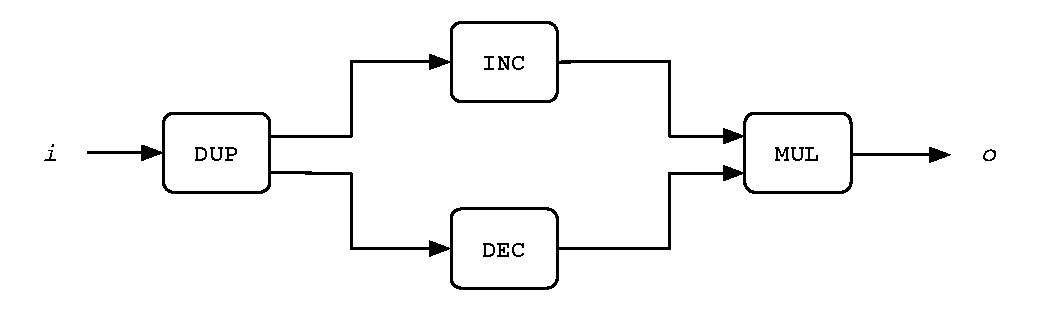
\includegraphics[width=0.75\textwidth]{figs/networkfour}
  \caption{A very simple dataflow network}
  \label{fig:networkfour}
\end{figure}

The network of Fig.~\ref{fig:networkfour} involves four simple actors. Actor \texttt{inc}
(resp. \texttt{inc}) adds (resp. substracts) 1 to each element of its input stream, actor
\texttt{mul} performs point-wise multiplication of two streams and actor \texttt{dup} duplicates its
input stream.

To understand what really ``happens'' when it is ``executed'' we need to attach a
\emph{semantics} both to actors and to the channels connecting these actors.

\medskip
The semantics of actors will be given as a set of \emph{firing rules} describing exactly \emph{when}
an actor executes (``fires'') and \emph{what} happens then. In this first example, the firing rule is the
same for each actor and it can be stated as : whenever a token is available on the channel connected
to each input port then read (``consume'') this token, compute the result(s) from the associated
value(s) and write (``produce'') the token(s) carrying this (these) result(s) on the channels
connected to the output port(s)\footnote{We will see latter that \caph allows more complex rules
  (and hence more sophisticated behaviors) to be expressed.}.

\medskip
The semantics of channels is simple : they will be viewed as FIFOs (First In First Out) buffers. In the
final implementation, the size of theses FIFOs will obviously be an important parameter. But for
now, let us consider that they are essentially unbounded.

\section{From sketch to code}
\label{sec:first-lines-code}

There's a long way from the rather ``informal'' description of an application as given in 
Fig.~\ref{fig:networkfour} to a FPGA configuration performing the described functionnality on a
stream of values.

The main steps in this path are illustrated in Fig.~\ref{fig:toolset}. These steps will be discussed
in part 2 and 3 of this document. Let's focus for the moment in the initial step, which is 
writing the source code of the application using the \caph language.

\begin{figure}[h]
  \centering
  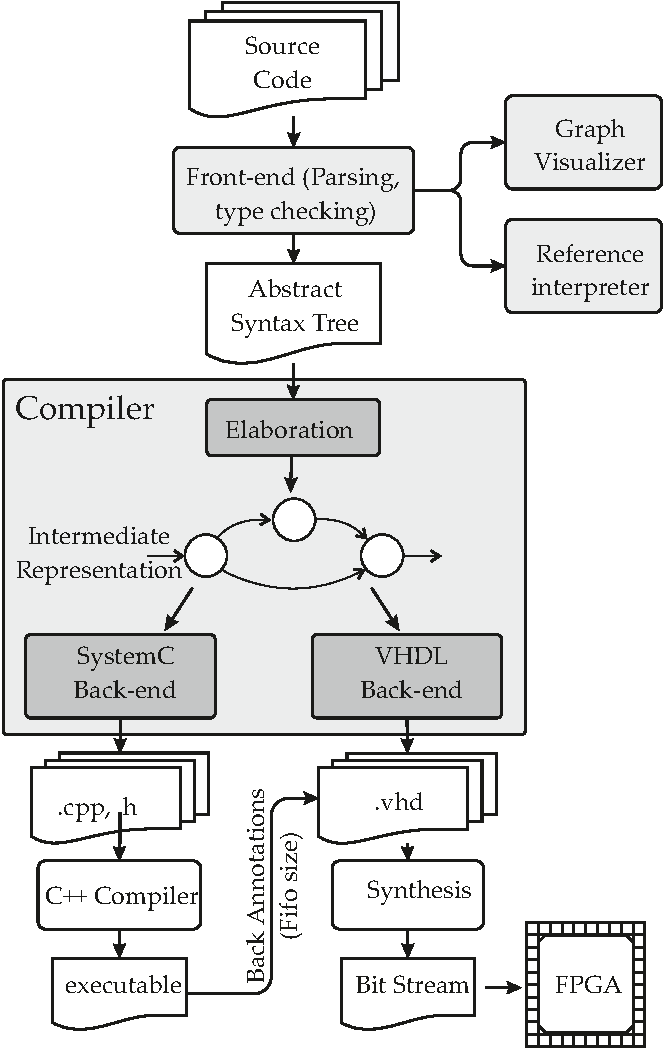
\includegraphics[width=0.4\textwidth]{figs/toolset}
  \caption{The CAPH design flow}
  \label{fig:toolset}
\end{figure}

\section{Writing the source code}
\label{sec:writing-source-code}

Let's write in \caph the description of the application depicted
in Fig.~\ref{fig:networkfour} in file \texttt{simple.cph}.

\medskip
We start by declaring the input and the output of the network :

\begin{lstlisting}[style=CaphStyle]
stream inp: unsigned<8> from "sample.txt";
stream outp: unsigned<8> to "result.txt";
\end{lstlisting}

The keyword \texttt{stream} introduces an I/O declaration. Each I/O has a name, a type and a
description. Here, we declare
\begin{itemize}
\item \texttt{inp} to be a input, with type \verb|unsigned<8>|, \emph{i.e.}
unsigned 8-bit integer, taking  values from a a file named \texttt{sample.txt}\footnote{As said
  above, this file will be used for simulation.}. 
\item \texttt{outp} to be an output, also with type \verb|unsigned<8>| putting values in a file
  named \texttt{result.txt}.
\end{itemize}

Concerning syntax, note that each declaration ends with a semi-colon.

\medskip
The next step consists in describing the network of actors. Basically, this involves specifying
which actors appear in this network and listing the connexions between these actor (``wiring'' the
network). In \caph\footnote{And for reasons which are advocated in the reference
  manual~\cite{caph-lrm}.}, this is done in a purely textual manner, by naming wires and viewing
actors as functions from wires to wires.

In this particular case, we start with the following declaration : 

\begin{lstlisting}[style=CaphStyle]
net (x1,x2) = dup inp;
\end{lstlisting}

This declaration, introduced by the \verb|net| keyword actually has two effects :
\begin{itemize}
\item first, it creates, in the network described by the program, a node named \texttt{dup},
\item second, it respectively \emph{binds} the input of this node to the wire named \emph{inp}
  (which, in this case is the input wire of the whole network) and  its outputs to two wires named
  \verb|x1| and \verb|x2|.
\end{itemize}

\medskip
We can now proceed (going ``from left to right'' in the graph of Fig.~\ref{fig:networkfour}), with
the following declarations : 

\begin{lstlisting}[style=CaphStyle]
net y1 = inc x1;
net y2 = dec x2;
\end{lstlisting}

The first declaration insert a nodes name \texttt{inc}, binding its 
input to the previously defined \texttt{x1} wire (\emph{i.e.} the first output of the \texttt{dup}
node) and its output to a new wire named \texttt{y1}. The second one does a similar thing with node
\texttt{dec} and wires \texttt{x2} and \texttt{y2} respectively.

\medskip
A last declaration inserts the \texttt{mul} node, connecting its inputs to the output of the
\texttt{inc} (resp. \texttt{dec}) node (by means of wires \texttt{y1} and \texttt{y2})  and its
output to the global output \texttt{outp} :

\begin{lstlisting}[style=CaphStyle]
net outp = mul (y1,y2);
\end{lstlisting}

\medskip
Note that the last three declarations could have been combined into a single one by writing :

\begin{lstlisting}[style=CaphStyle]
net outp = mul (inc x1, dec x2);
\end{lstlisting}

Which style is better -- with or without explicit naming of intermediate wires -- is essentially a
matter of taste since both will lead to exactly the same network. 

\medskip Together, the set of \texttt{stream} and \texttt{net} declarations introduced above
completely determines the \emph{static} stucture of the actor network\footnote{In other words, its
  \emph{topology}}.

\medskip
We now have to define the \emph{dynamic} behavior of the actors appearing in this network.

Let's start with the \texttt{inc} actor. Its behavior is specified by the following declaration :

\begin{lstlisting}[style=CaphStyle,numbers=left,numberstyle=\tiny]
actor inc
  in (i: unsigned<8>)
 out (o: unsigned<8>)
rules
| i:x -> o:x+1;
\end{lstlisting}

This declaration is composed of two parts : The first part (the \emph{interface}, lines 1--3) gives
the name of the actor and lists its inputs and outputs (giving a name and a type to each of them),
The second part (lines 4--5) specifies the behavior of the actor, by listing all the associated
firing rules. Here, there's only one rule\footnote{Each rule starts with a leading \texttt{|}.} and
it can be read as follows : whenever there's a token, carrying a value $x$, available on input
\texttt{i} then read (consumes) this token and write a token carrying value $x+1$ on output
\texttt{o}.

\medskip 
The definition of the \texttt{dec} actor is very similar : 

\begin{lstlisting}[style=CaphStyle]
actor dec
  in (i: unsigned<8>)
 out (o: unsigned<8>)
rules
| i:x -> o:x-1;
\end{lstlisting}

\medskip
The \texttt{mul} actor has two inputs and a single input. This is reflected in its interface and in
the format of the firing rule :

\begin{lstlisting}[style=CaphStyle]
actor mul
  in (i1: unsigned<8>, i2:unsigned<8>)
 out (o: unsigned<8>)
rules
| (i1:x, i2:y) -> o:x*y;
\end{lstlisting}

The interpretation of the firing rule for the \texttt{mul} actor is an obvious generalisation of the
one given for the two previous actors : the actor fires whenever a token (carrying values $x$ and
$y$ respectively) is available on \texttt{inputs}, \texttt{i1} and \texttt{i2}.  Concerning the
syntax, note the use of brackets on the left-hand side of the rule, which is mandatory here.

\medskip
The \texttt{dup} actor has a single input, but two outputs. This, again, is reflected in its
interface and the format of the firing rule :

\begin{lstlisting}[style=CaphStyle]
actor dup
  in (i: unsigned<8>)
 out (o1: unsigned<8>, o2:unsigned<8>)
rules
| i:x -> (o1:x, o2:x);
\end{lstlisting}

For this token, a token, carrying the same value ($x$) will be produced on both outputs
(\texttt{o1} and \texttt{o2}) whenever the actor fires.

\medskip
The full text of the program is given in Listing~\ref{lst:simple-full}. Note that, contrary to the
presentation order we have used above, the declarations of actors actually have to appear first
(this is because these declarations will be used by the \texttt{net} declarations). Comments are
introduced by the \verb|--| character sequence\footnote{Comments are single-line, like in Java.}. 

\begin{lstlisting}[style=CaphStyle,caption={Complete CAPH source code for the application
    depicted in Fig.~\ref{fig:networkfour}},label={lst:simple-full}]
-- Actor declarations

actor inc
  in (i: unsigned<8>)
 out (o: unsigned<8>)
rules
| i:x -> o:x+1;

actor dec
  in (i: unsigned<8>)
 out (o: unsigned<8>)
rules
| i:x -> o:x-1;

actor mul
  in (i1: unsigned<8>, i2:unsigned<8>)
 out (o: unsigned<8>)
rules
| (i1:x, i2:y) -> o:x*y;

actor dup
  in (i: unsigned<8>)
 out (o1: unsigned<8>, o2:unsigned<8>)
rules
| i:x -> (o1:x, o2:x);

-- I/O declarations

stream inp: unsigned<8> from "sample.txt";
stream outp: unsigned<8> to "result.txt";

-- Network declarations

net (x1,x2) = dup inp;
net y1 = inc x1;
net y2 = dec x2;
net outp = mul (y1,y2);
\end{lstlisting}

%%% Local Variables: 
%%% mode: latex
%%% TeX-master: "caph-primer"
%%% End: 

%%%%%%%%%%%%%%%%%%%%%%%%%%%%%%%%%%%%%%%%%%%%%%%%%%%%%%%%%%%%%%%%%%%%%%%%%%%%%%%%%%%%%%%%%
%%                                                                                     %%
%%                This file is part of the CAPH Compiler distribution                  %%
%%                            http:%/caph.univ-bpclermont.fr                           %%
%%                                                                                     %%
%%                                  Jocelyn SEROT                                      %%
%%                         Jocelyn.Serot@univ-bpclermont.fr                            %%
%%                                                                                     %%
%%         Copyright 2011-2018 Jocelyn SEROT.  All rights reserved.                    %%
%%  This file is distributed under the terms of the GNU Library General Public License %%
%%      with the special exception on linking described in file ..%LICENSE.            %%
%%                                                                                     %%
%%%%%%%%%%%%%%%%%%%%%%%%%%%%%%%%%%%%%%%%%%%%%%%%%%%%%%%%%%%%%%%%%%%%%%%%%%%%%%%%%%%%%%%%%

\chapter{Dealing with images}
\label{cha:lang-images}

In this chapter we will show how to use CAPH to implement a very simple image processing application.
This will be the opportunity to introduce the core concepts used for dealing with images -- mainly
their representation as \emph{structured streams} of pixels -- and to describe the tools used for
manipulating them at the simulation level.

\section{Representation of images}
\label{sec:repr-imag}

In chapter~\ref{cha:lang-basic}, the dataflow network used as an example, was operating on a raw,
unstructured stream of data. In contrast, images are \emph{structured} streams of pixels. In
particular, in most of applications, we need a way to encode the dimensions of a given image (so
that we can tell, for example, if a stream of 64 pixels actually represents an image with 8 lines of
8 pixels, an image with 4 lines of 16 pixels or even four successive images with 4 lines of 4
pixels).

For this, the idea is to insert, in the stream of pixels, \emph{control} tokens expliciting the
underlying structure of the data and to distinguish control tokens from \emph{data} tokens (carrying
pixel values) by attaching a \emph{tag} to each token. In practice, for an application having to
process images, the input of will be a sequential stream of tokens, where each
single token is either
\begin{itemize}
\item the tag \verb|SoI| (start of image),
\item the tag \verb|EoI| (end of image),
\item the tag \verb|SoL| (start of line),
\item the tag \verb|EoL| (end of line),
\item a pixel value, with tag \verb|Pixel|.
\end{itemize}

With this scheme, the $4 \times 4$ image depicted in Fig.~\ref{fig:img4}, for example, will be
represented (``encoded'') by the following stream of tokens:

%\footnotesize
\begin{center}
\begin{spverbatim}
SoI SoL Pixel(10) Pixel(30) Pixel(55) Pixel(90) EoL SoL Pixel(33) Pixel(53)
Pixel(60) Pixel(12) EoL SoL Pixel(99) Pixel(56) Pixel(23) Pixel(11) EoL SoL
Pixel(11) Pixel(82) Pixel(46) Pixel(11) EoL  EoI
\end{spverbatim}
\end{center}
%\normalsize

\begin{figure}[h]
  \centering
  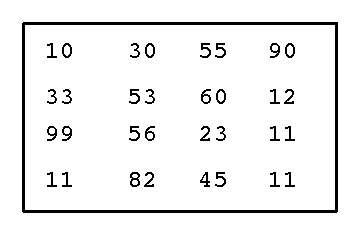
\includegraphics[width=0.25\linewidth]{figs/img4}
  \caption{A $4 \times 4$ image}
  \label{fig:img4}
\end{figure}

In fact, only two distinct control tokens are needed :

\begin{itemize}
\item a token \verb|SoS| (\emph{start of structure}), signaling the start of an image or the start
  of a line within a image,
\item a token \verb|EoS| (\emph{end of structure}), signaling the end of an image or the end
  of a line within a image.
\end{itemize}

As a result, and using the following abbreviations :
\begin{itemize}
\item \verb|<| for \verb|SoS|,
\item \verb|>| for \verb|Eos|,
\item \verb|v| for \verb|Pixel(v)|,
\end{itemize}

the image depicted in Fig.~\ref{fig:img4}, can be represented by the following stream of tokens~:

%\footnotesize
\begin{center}
\begin{spverbatim}
< < 10 30 55 90 > < 33 53 60 12 > < 99 56 23 11 > < 11 82 46 11 > >
\end{spverbatim}
\end{center}
%\normalsize

\section{Processing images}
\label{sec:processing-images}

By using the pattern-matching mechanism introduced in Chap.~\ref{cha:lang-basic} it is
very easy to describe the behavior of actors operating on structured streams of values. 

\medskip
Consider, for example, an actor performing image negation on images made of 8-bit unsigned pixels,
\emph{i.e.} each pixel having value $v$ is transformed to a pixel having value $255-v$. 

Such an actor is decribed in Listing~\ref{lst:inv-actor}. 

First, note that the type of the input and output for this actor (\verb|i| and \verb|o|, lines 2--3)
is \emph{not}

\begin{center}
\verb|unsigned<8>|
\end{center}

but

\begin{center}
\verb|unsigned<8> dc|
\end{center}

 The type \verb|dc| (abbreviation for \emph{data or
  control}) is here used for representing structured values\footnote{CAPH uses so-called
  \emph{algebraic data types} (aka \emph{variant types}) for this. Internally, the \texttt{dc} type
  constructor is defined as : 

\texttt{type \$t dc = SoS | EoS | Data of \$t}

where \texttt{SoS}, \texttt{EoS} and \texttt{Data} are the \emph{value
  constructors} associated to tags and $\$t$ denotes a \emph{type variable}. The notations
\texttt{'<}, \texttt{'>} and \texttt{'v} are then abbreviations for \texttt{SoS}, \texttt{EoS} and
\texttt{Data v} respectively.}.
A value having type \verb|t dc|, where
\verb|t| is a scalar (unstructured) type, is either
\begin{itemize}
\item the control value \verb|SoS| (which can be abbreviated as \verb|'<|),
\item the control value \verb|EoS| (which can be abbreviated as \verb|'>|),
\item a data value \verb|v|, of type \verb|t| (which can be abbreviated as \verb|'v|).
\end{itemize}

The actor rules use the pattern matching mechanism to inspect the tag of
the input value and to produce the appropriate value on output :
\begin{itemize}
\item if the input token is a control token (\verb|'<| or \verb|'>|, lines 5 or 6), write the same token on output
  (this means that the \emph{structure} of the image is unchanged),
\item if the input token is data token (pixel), carrying value \verb|x| (line 7), write a data token
  carrying value \verb|255-x| on output.
\end{itemize}

\begin{lstlisting}[style=CaphStyle,numbers=left,numberstyle=\tiny,caption={An actor computing image negatives in
    CAPH},label={lst:inv-actor}]
actor inv
  in (i: unsigned<8> dc)
 out (o: unsigned<8> dc)
rules
| i:'< -> o:'<;
| i:'> -> o:'>;
| i:'x -> o:'255-x;
\end{lstlisting}

\medskip
\textbf{Note 1}. The code in Listing~\ref{lst:inv-actor} uses the abbreviated syntax for denoting
values with type \verb|unsigned<8> dc|. It is also possible to use the un-abbreviated syntax, as
shown in Listing.~\ref{lst:inv-actor2}. 

\begin{lstlisting}[style=CaphStyle,caption={An actor computing image negatives in
    CAPH (alternate syntax)},label={lst:inv-actor2}]
actor inv
  in (i: unsigned<8> dc)
 out (o: unsigned<8> dc)
rules
| i:SoS -> o:SoS;
| i:EoS -> o:EoS;
| i:Data(x) -> o:Data(255-x);
\end{lstlisting}

\medskip
\textbf{Note 2}. The CAPH type system ensures that tagged and untagged values are used consistently
in programs. It we write, for example, the last rule of actor \verb|inv| as :

\begin{lstlisting}[style=CaphStyle]
| i:x -> o:255-x;
\end{lstlisting}

we get the following error message from the compiler :

\begin{lstlisting}[style=BashOutputStyle]
File "inv.cph", line 7, characters 11-16:
>| i:x -> o:255-x;
>...........^^^^^
An error occured when typing this expression: types unsigned<#a> and unsigned<8> dc cannot be unified.
\end{lstlisting}

What the type checker detects here is that the output \verb|o|, supposed to have type
\verb|unsigned<8> dc| (\emph{i.e.} to be assigned a tagged value) is actually assigned a value of
type \verb|unsigned<n>|\footnote{The notation \texttt{\#a} designates a \emph{size variable}. It
  basically means "any, unknown, size n".} (\emph{i.e.} the untagged value $255-x$). 

\bigskip
In chapter~\ref{cha:cl-images}, we will describe the implementation, simulation and synthesis of an
application making use of the \verb|inv| actor.


%%% Local Variables: 
%%% mode: latex
%%% TeX-master: "caph-primer"
%%% End: 

%%%%%%%%%%%%%%%%%%%%%%%%%%%%%%%%%%%%%%%%%%%%%%%%%%%%%%%%%%%%%%%%%%%%%%%%%%%%%%%%%%%%%%%%%
%%                                                                                     %%
%%                This file is part of the CAPH Compiler distribution                  %%
%%                            http:%/caph.univ-bpclermont.fr                           %%
%%                                                                                     %%
%%                                  Jocelyn SEROT                                      %%
%%                         Jocelyn.Serot@univ-bpclermont.fr                            %%
%%                                                                                     %%
%%         Copyright 2011-2018 Jocelyn SEROT.  All rights reserved.                    %%
%%  This file is distributed under the terms of the GNU Library General Public License %%
%%      with the special exception on linking described in file ..%LICENSE.            %%
%%                                                                                     %%
%%%%%%%%%%%%%%%%%%%%%%%%%%%%%%%%%%%%%%%%%%%%%%%%%%%%%%%%%%%%%%%%%%%%%%%%%%%%%%%%%%%%%%%%%

\chapter{Image processing}
\label{cha:lang-ip}

In this last chapter, we describe the use of the \caph language to implement a more ``realistic'' image
processing application.

\medskip
This application performs edge extraction on images using the
well-known Sobel filter.

An example of input and output image is given Fig.~\ref{fig:pcb-ex}.

\begin{figure}[h]
\centering
  \begin{tabular}[c]{cc}
  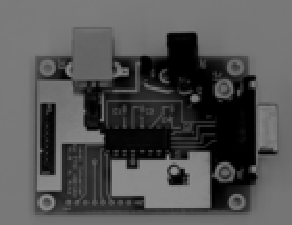
\includegraphics[width=0.2\textwidth]{figs/pcb.pdf} &
  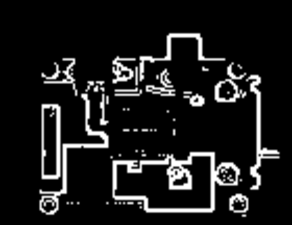
\includegraphics[width=0.2\textwidth]{figs/pcb-res.pdf} \\
  Input image & Result image
  \end{tabular}
  \caption{Edge extraction with the Sobel operator}
  \label{fig:pcb-ex}
\end{figure}

For each pixel $P_{i,j}$ of the input image, the magnitude of the local gradient is computed using
approximations of the horizontal and vertical derivatives $G_x$ and $G_y$, and the resulting value
is compared to a fixed threshold for producing a binary image (with edge pixels encoded as 1 and
background pixels as 0). To simplify, the magnitude of the gradient, $G=\sqrt{G_x^2+G_y^2}$, will be
here approximated as $|G_x|+|G_y|/2^n$, where $n$ is a scaling factor.

Considering we have three actors, \verb|grad|, \verb|asum|, \verb|thr|, computing respectively the
gradient components, the half sum their absolute values and the binarisation of an image, the dataflow
formulation of the corresponding is given in Listing~\ref{lst:sobel-1}.  Figure~\ref{fig:sobel-dot}
gives the corresponding dataflow network\footnote{The binarisation threshold has here been
  arbitrarily set to 20.}

\begin{figure}[htbp]
  \centering
 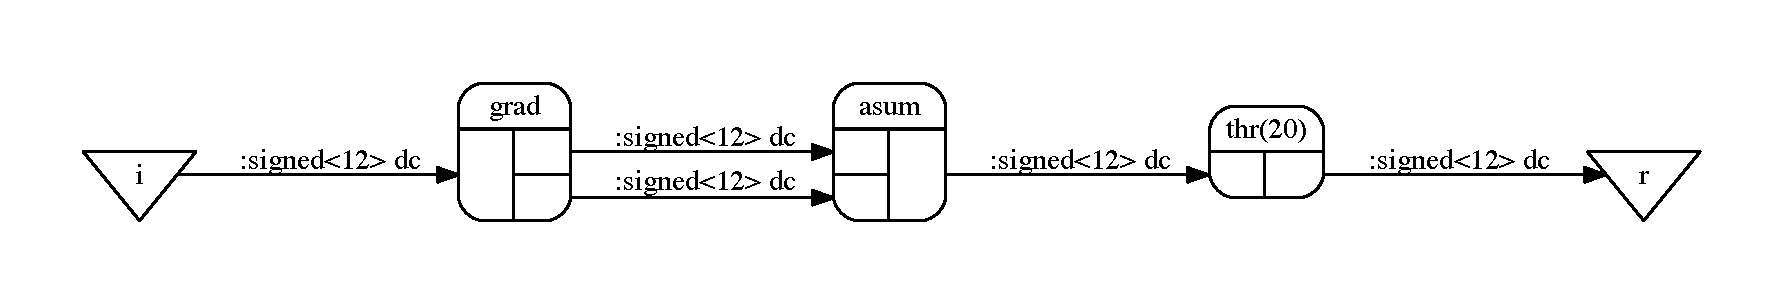
\includegraphics[width=0.9\textwidth]{./figs/sobel-dot.pdf}
  \caption{The graphical representation of the program given in Listing.~\ref{lst:sobel-full}}
  \label{fig:sobel-dot}
\end{figure}

\begin{lstlisting}[style=CaphStyle,numbers=left,numberstyle=\tiny,caption={A Sobel edge extraction
    application in Caph (top level description)},label={lst:sobel-1}]
actor grad in (i:signed<s> dc) out(o1:signed<s> dc, o2:signed<s> dc) ...
actor asum in ( i1:signed<s> dc, i2:signed<s> dc) out( o:signed<s> dc)  ...
actor thr (k:signed<s>) in ( i:signed<s> dc) out( o:unsigned<s> dc) ...

stream i:signed<12> dc from "pcb.txt";
stream r:signed<12> dc to "result.txt";

net (gx,gy) = grad i;         -- gradient x and y components
net gm = asum (gx, gy);       -- gradient magnitude (approx)
net r = thr 20 gm;
\end{lstlisting}

\medskip
The \verb|thr| actor is described in Listing~\ref{lst:sobel-thr}. This actor applies a binarisation
threshold to an image, returning a image of 1-bit unsigned pixels. The binarisation threshold is
specified as a parameter (\verb|t|, line 1), whose value will be set when instanciating the actor at
the network level (see line 10 in Listing.~\ref{lst:sobel-1}). Binarisation is performed by simply
comparing each pixel value to the threshold (last rule, line 7). 

\begin{lstlisting}[style=CaphStyle,numbers=left,numberstyle=\tiny,caption={The \texttt{thr} actor in
    Caph},label={lst:sobel-thr}]
actor thr (k:signed<s>)
  in ( i:signed<s> dc)
  out( o:unsigned<1> dc)
rules i -> o
| '< -> '<
| '> -> '>
| 'p -> if p>k then '1 else '0
;
\end{lstlisting}

\medskip The \verb|asum| actor is described in Listing~\ref{lst:sobel-magn}. This actor takes the
computes an approximation of the gradient magnitude by summing the absolute value of its two
components and dividing it by 2. The computation of the absolute value is
performed using the global function \verb|fabs|, which is declared before the actor.  The division
by 2 is implemented using the bit-shift builtin operator \verb|>>|.

\begin{lstlisting}[style=CaphStyle,numbers=left,numberstyle=\tiny,caption={The \texttt{asum} actor in
    Caph},label={lst:sobel-magn}]
function fabs x = if x < 0 then -x else x : signed<s> -> signed<s>;

actor asum
  in ( i1:signed<s> dc, i2:signed<s> dc)
  out( o:signed<s> dc)
rules (i1,i2) -> o
| ('<,'<) -> '<
| ('>,'>) -> '>
| ('p,'q) -> '(fabs(p)+fabs(q))>>1
;
\end{lstlisting}

\medskip
The computation of the gradient components could be carried out by writing out dedicated actors, in the
vein of those described in Sec.~2.5 of the reference manual. We will here adopt a more straightforward
approach and rely on the predefined convolution actors provided in the standard CAPH library. The
gradient $x$ and $y$ component can be computed by convolving the input image with the 2D kernels
showed in Fig.~\ref{fig:sobel-kernels}.

\begin{figure}[h]
\centering
  \begin{tabular}[c]{cc}
$ G_x = \begin{pmatrix}
      1 & 0 & -1 \\
      2 & 0 & -2 \\
      1 & 0 & -1 \\
    \end{pmatrix} $ &
$ G_y = \begin{pmatrix}
      1 & 2 & 1 \\
      0 & 0 & 0 \\
      1 & 2 & 1 \\
    \end{pmatrix} $
  \end{tabular}
  \caption{Convolution kernels for computing the gradient $x$ and $y$ components}
  \label{fig:sobel-kernels}
\end{figure}

For this, the file \verb|convol.cph| provides the actor \verb|conv233|. This actor accepts three
parameters~:
\begin{itemize}
\item a convolution kernel, given as a 2D array $k[0..2][0..2]$
\item a scaling factor $n$,
\item a padding value $v$.
\end{itemize}
Given a $M\times N$ input image $x$, represented as a structured stream 

\begin{center}
\begin{math}
<\ <\ x_{1,1}\ x_{1,2}\ ...\ x_{1,N}\ >\ <\ x_{2,1}\ x_{2,2}\ ...\ x_{2,N}\ >\ ...\ <\ x_{M,1}\ x_{M,2}\ ...\ x_{M,N}\ >\ >
\end{math}
\end{center}

\noindent
the \verb|conv233| actor computes an output image $y$, with the same representation and dimensions

\begin{center}
\begin{math}
<\ <\ y_{1,1}\ y_{1,2}\ ...\ y_{1,N}\ >\ <\ y_{2,1}\ y_{2,2}\ ...\ y_{2,N}\ >\ ...\ <\ y_{M,1}\ y_{M,2}\ ...\ y_{M,N}\ >\ >
\end{math}
\end{center}

\noindent
where 

\begin{equation}
y_{i,j} = 
\begin{cases}
v & \text{if}\ 1 \leq 2\ \text{or}\ 1 \leq j \leq 2 \\
\sum\limits_{\substack{0\leq i'\leq 2\\ 0\leq j'\leq 2\}}} k_{2-i',2-j'}.x_{i-i',j-j'}\quad /2^n & \text{if}\ 2\leq i\leq M\ \text{and}\ 2\leq j \leq N
\end{cases}
\label{eq:conv233}
\end{equation}

The corresponding formulation in CAPH is given in Listing~\ref{lst:sobel-conv}. The convolution
kernels $G_x$ and $G_y$ are specified as 2S arrays. The padding value $v$
(for the first two lines and columns) has here been set to 0 and the scaling factor is also 0.

\begin{lstlisting}[style=CaphStyle,numbers=left,numberstyle=\tiny,caption={Computation of the
    gradient components using the \texttt{conv233} actor of the standard CAPH library},label={lst:sobel-conv}]
net gx = conv233 ([[1,0,-1], [2,0,-2], [1,0,-1]], 0, 0) i;  -- grad x component
net gy = conv233 ([[1,2,1], [0,0,0], [-1,-2,-1]], 0, 0) i;  -- grad y component
\end{lstlisting}

\medskip
The complete source code of the application is given in
Listing~\ref{lst:sobel-full}\footnote{It can also be found in directory
  \texttt{examples/working/primer/sobel} of the distribution.}. The corresponding dataflow graph is
given in Fig.~\ref{fig:sobel-full}. To simplify further assessment, the name of the input file and
the binarisation threshold are here specified indirectly by using references to \emph{macros}.
The corresponding values will be set
when invoking the compiler (with the \verb|-D| option), thus
offering a way of changing them without having to edit the source file (see Sec.~9.9 of the manual).

\begin{lstlisting}[style=CaphStyle,numbers=left,caption={Complete source code of the Sobel-based
    edge extraction},label={lst:sobel-full}]
#include "convol.cph"

function fabs x = if x < 0 then -x else x : signed<s> -> signed<s>;

actor asum
  in ( i1:signed<s> dc, i2:signed<s> dc)
  out( o:signed<s> dc)
rules (i1,i2) -> o
| ('<,'<) -> '<
| ('>,'>) -> '>
| ('p,'q) -> '(fabs(p)+fabs(q))>>1
;

actor thr (k:signed<s>)
  in ( i:signed<s> dc)
  out( o:unsigned<1> dc)
rules i -> o
| '< -> '<
| '> -> '>
| 'p -> if p>k then '1 else '0
;

stream i:signed<12> dc from %ifile;
stream r:unsigned<1> dc to "result.txt";

net gx = conv233 ([[1,0,-1],
                   [2,0,-2],
                   [1,0,-1]],0,0) i;    -- grad x component
net gy = conv233 ([[1,2,1],
                   [0,0,0],
                   [-1,-2,-1]],0,0) i;  -- grad y component
net gm = asum (gx, gy);                 -- grad amplitude (approx)
net r = thr %threshold gm;
\end{lstlisting}

\begin{figure}[htbp]
  \centering
 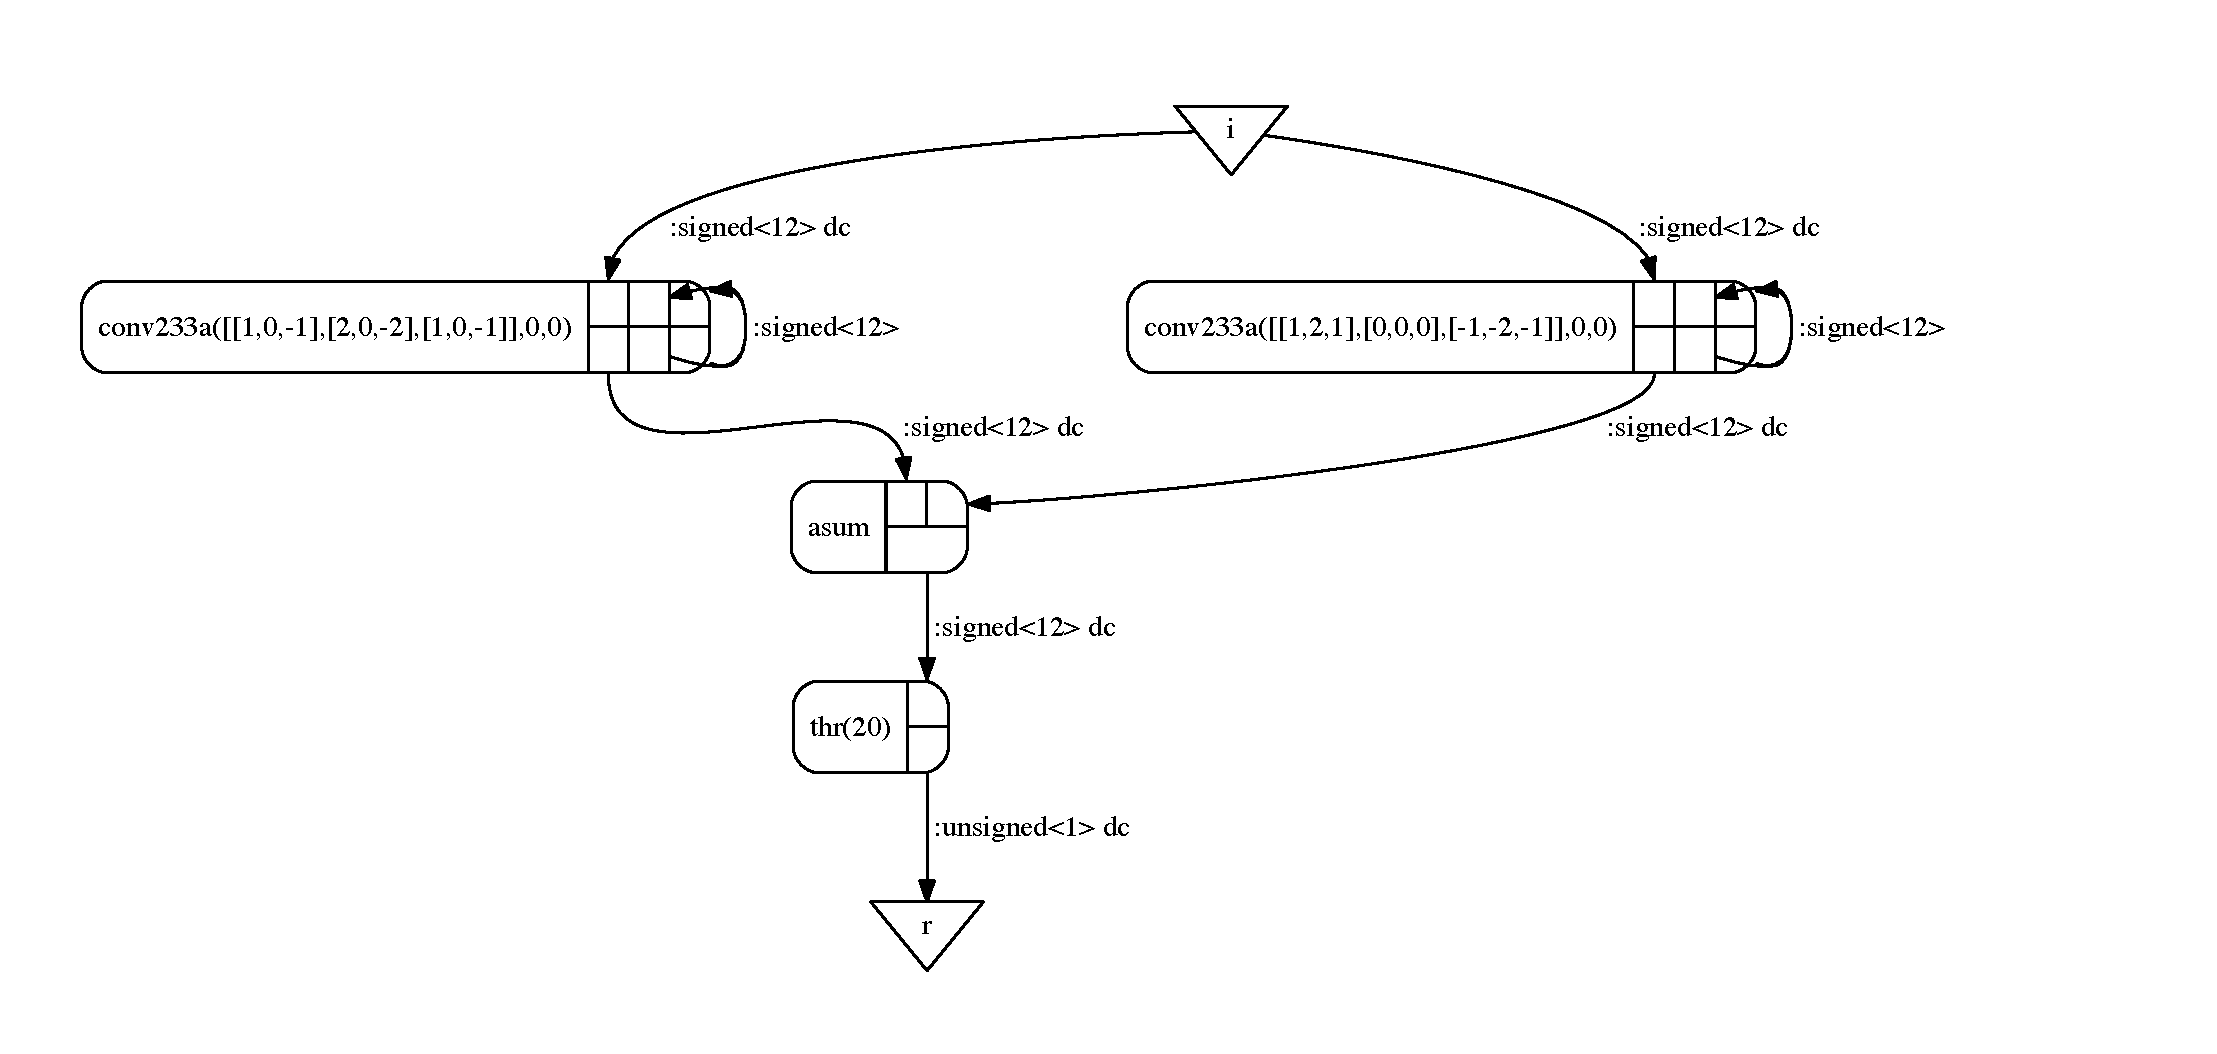
\includegraphics[width=\textwidth]{./figs/sobel-full.pdf}
  \caption{The graphical representation of the program given in Listing.~\ref{lst:sobel-full}}
  \label{fig:sobel-full}
\end{figure}

\bigskip
As for the application of the previous chapter, we will describe the implementation, simulation and
synthesis of this application in part 3 of this document.

%%% Local Variables: 
%%% mode: latex
%%% TeX-master: "caph-primer"
%%% End: 

\part{The Caph IDE}
%%%%%%%%%%%%%%%%%%%%%%%%%%%%%%%%%%%%%%%%%%%%%%%%%%%%%%%%%%%%%%%%%%%%%%%%%%%%%%%%%%%%%%%%%
%%                                                                                     %%
%%                This file is part of the CAPH Compiler distribution                  %%
%%                            http:%/caph.univ-bpclermont.fr                           %%
%%                                                                                     %%
%%                                  Jocelyn SEROT                                      %%
%%                         Jocelyn.Serot@univ-bpclermont.fr                            %%
%%                                                                                     %%
%%         Copyright 2011-2018 Jocelyn SEROT.  All rights reserved.                    %%
%%  This file is distributed under the terms of the GNU Library General Public License %%
%%      with the special exception on linking described in file ..%LICENSE.            %%
%%                                                                                     %%
%%%%%%%%%%%%%%%%%%%%%%%%%%%%%%%%%%%%%%%%%%%%%%%%%%%%%%%%%%%%%%%%%%%%%%%%%%%%%%%%%%%%%%%%%

\chapter*{Introduction}
\label{sec:ide-intro}

This part describes the \caph IDE. This IDE basically provides a Graphical user Interface (GUI) to
the \caphc compiler.

\medskip
The \caph IDE allows
\begin{itemize}
\item writing, reading and editing of \caph programs, % (\texttt{.cph}) (with syntax coloring),
\item grouping all files associated to a \caph program into \emph{projects},
\item generating and viewing graphical representations of these programs,
\item running simulations of these programs,
\item generating SystemC and VHDL code.
\end{itemize}

\medskip
\textbf{Note}. This document describes the Windows version of the \caph IDE. The IDE can also be built and used on
Unix-based systems (Linux, MacOS).

%%% Local Variables: 
%%% mode: latex
%%% TeX-master: "caph-primer"
%%% End: 

%%%%%%%%%%%%%%%%%%%%%%%%%%%%%%%%%%%%%%%%%%%%%%%%%%%%%%%%%%%%%%%%%%%%%%%%%%%%%%%%%%%%%%%%%
%%                                                                                     %%
%%                This file is part of the CAPH Compiler distribution                  %%
%%                            http:%/caph.univ-bpclermont.fr                           %%
%%                                                                                     %%
%%                                  Jocelyn SEROT                                      %%
%%                         Jocelyn.Serot@univ-bpclermont.fr                            %%
%%                                                                                     %%
%%         Copyright 2011-2018 Jocelyn SEROT.  All rights reserved.                    %%
%%  This file is distributed under the terms of the GNU Library General Public License %%
%%      with the special exception on linking described in file ..%LICENSE.            %%
%%                                                                                     %%
%%%%%%%%%%%%%%%%%%%%%%%%%%%%%%%%%%%%%%%%%%%%%%%%%%%%%%%%%%%%%%%%%%%%%%%%%%%%%%%%%%%%%%%%%

\chapter{Basic usage}
\label{cha:ide-basic}

We will illustrate how to write, compile and simulate with the \caph IDE with a very simple \caph
program, even simpler than that used in Part 1. This program is reproduced in
Listing~\ref{lst:ide-sample-pgm}.  It involves a single actor, named \texttt{scale}, which
multiplies by \texttt{k} each value read on its input port \texttt{i} and writes the result on its
output port \texttt{o}. This actor is instanciated once, with \texttt{k=2}, and will read inputs
from file \verb|sample.txt| and write outputs to file \verb|result.txt|.

\begin{lstlisting}[style=CaphStyle,caption={A very simple program for testing the \caph IDE},label={lst:ide-sample-pgm}]
actor scale (k: unsigned<8>)
  in (i:unsigned<8>)
  out (o:unsigned<8>)
rules i -> o
| x -> k*x
;

stream inp:unsigned<8> from "sample.txt";
stream outp:unsigned<8> to "result.txt";

net outp = scale 2 inp;
\end{lstlisting}

\medskip
First, \textbf{launch the \caph application} by clicking on its icon in the installation directory or
directly from the Windows \emph{Start} menu. 

\medskip
The application main window is shown in Fig.~\ref{fig:main-window}. 
The main elements are (with corresponding areas labeled in red in Fig.~\ref{fig:main-window}) :
\begin{enumerate}
\item a menubar
\item four buttons for file manipulation; from left to right
  \begin{itemize}
  \item create a new file,
  \item open an existing file,
  \item save a file,
  \item save all files.
  \end{itemize}
\item five buttons to invoke the compiler for
  \begin{itemize}
  \item generating the dataflow graph representation of the current program and visualize it (button \textsc{graph}),
  \item simulating the current program and visualize it (button \textsc{Simu}),
  \item generating SystemC code from the current program (button \textsc{SystemC}),
  \item generating VHDL code from the current program (button \textsc{VHDL}),
  \item generating XDF representation of the current program (button \textsc{XDF}).
  \end{itemize}
\item a tree view of the current project,
\item a tab for viewing and editing input source files,
\item a tab for viewing output files,
\item a log area, displaying issued command and outputs from the compiler.
\end{enumerate}

\begin{figure}[h]
  \centering
  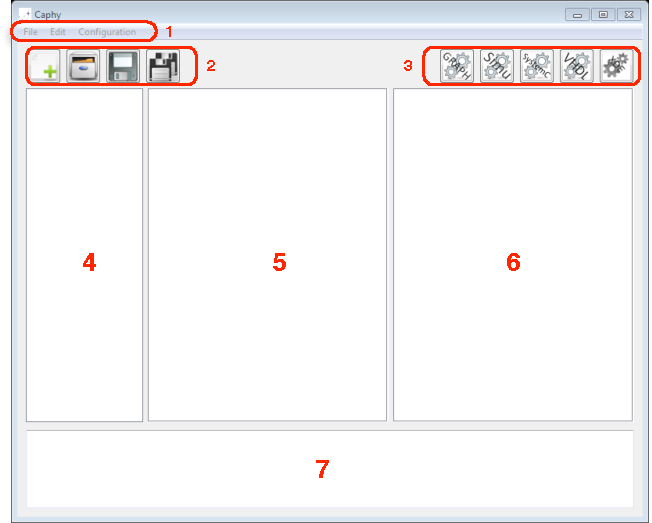
\includegraphics[width=0.75\textwidth]{figs/ide/main-window}
  \caption{\caphy main window}
  \label{fig:main-window}
\end{figure}

\medskip
Invoke the [\textsf{Configuration:Compiler and Tools}] menu item and check that the specified paths
are right (see Fig.~\ref{fig:config-window}). They should respectively point to 
\begin{itemize}
\item the location of the \texttt{caphc} compiler (\verb|<install>/bin/caphc|, where
  \verb|<install>| is the \caph installation directory, as specified during the installation
  process),
\item the location of the program to invoke for viewing \verb|.dot| graph files, 
\item the location of the program to invoke for viewing \verb|.pgm| image files. 
\end{itemize}
If the specified paths are not correct\footnote{This may be the case, for example, if you have
  changed the program to view graphs and/or images since \caph was installed.}, adjust them and click \textsc{Ok}.

\begin{figure}[h]
  \centering
  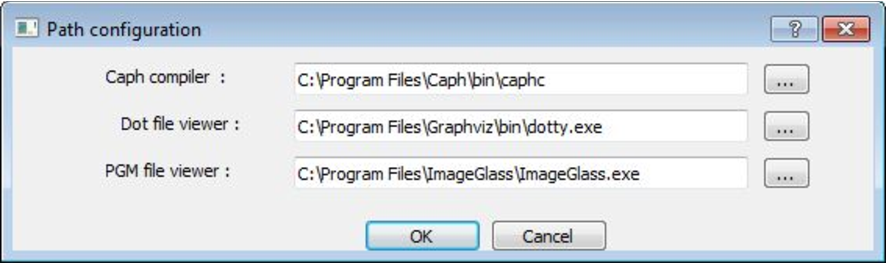
\includegraphics[width=0.75\textwidth]{figs/ide/config}
  \caption{Path configuration window}
  \label{fig:config-window}
\end{figure}

\medskip \textbf{Create a new source file} by clicking on the \textsf{New file} button (upper left)
or invoking the corresponding item of the \textsf{File} menu. A new tab will appear, named
\texttt{new} in the input files tab area. In this text tab, type\footnote{Or copy-paste} the program
reproduced in Listing~\ref{lst:ide-sample-pgm}, as illustrated in Fig.~\ref{fig:first-program}. 

\begin{figure}[h]
  \centering
  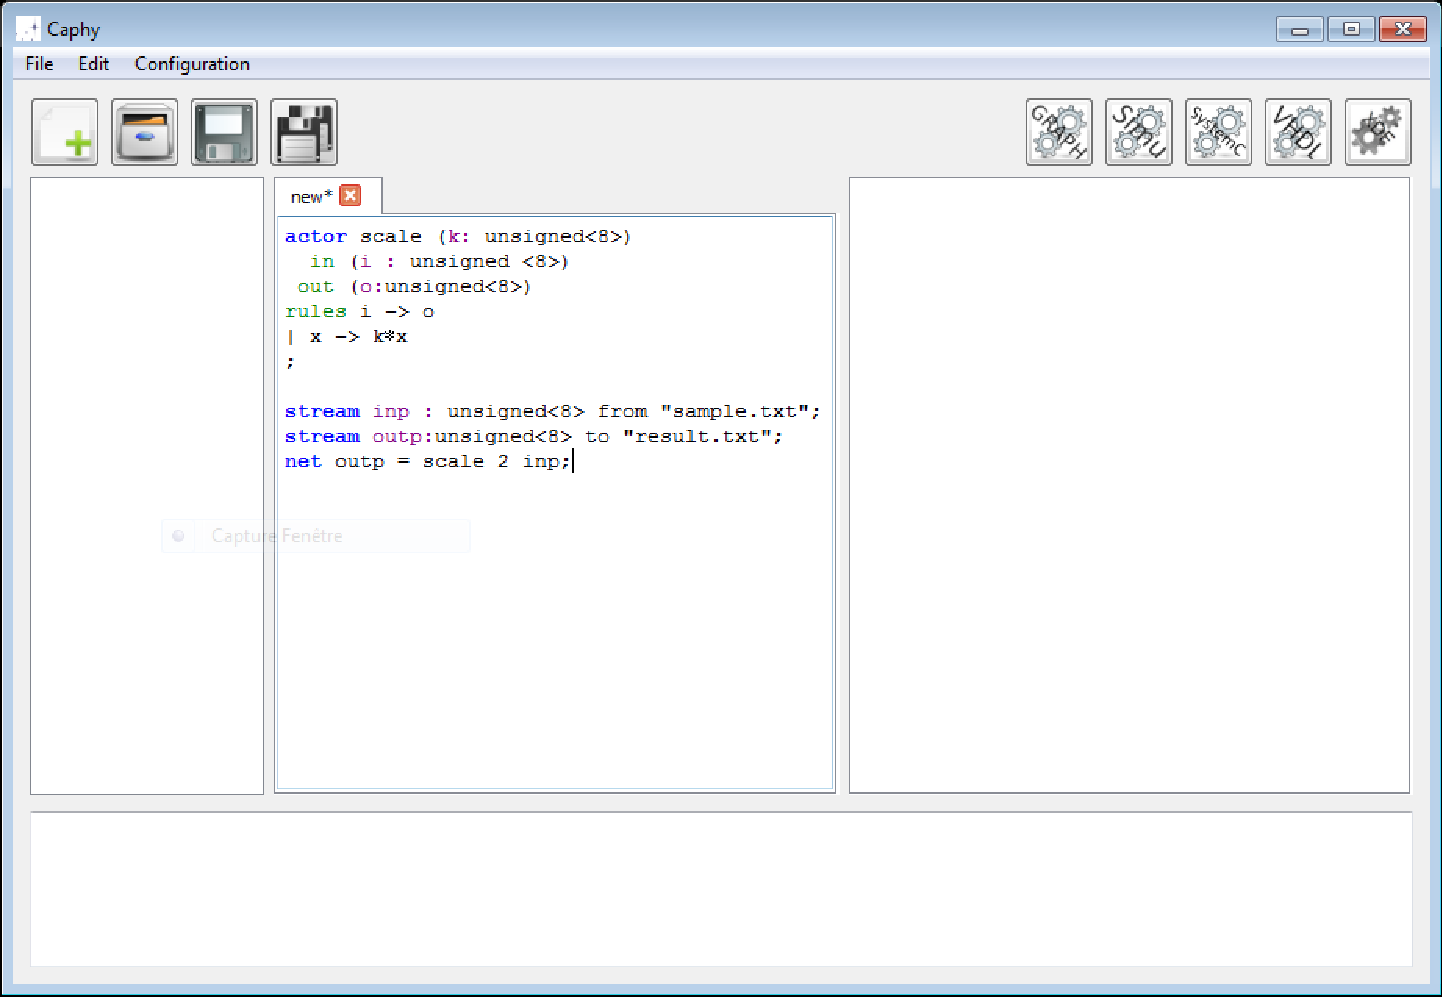
\includegraphics[width=0.75\textwidth]{figs/ide/first-program}
  \caption{Entering program}
  \label{fig:first-program}
\end{figure}

\medskip
\textbf{Save the program} by clicking on the \textsf{Save file} button or invoking the corresponding item of
the \textsf{File} menu. Be sure to use the \verb|.cph| filename suffix. Here we have saved it under
name \verb|main.cph|

\medskip
To \textbf{generate the graph}, clicking the \textsf{Graph} button (upper right). This will
\begin{itemize}
\item invoke the \caph compiler with the adequate option(s),
\item generate the \texttt{.dot} result file (in the same directory as the source file),
\item view this result by invoking the graph visualisation program specified in 
  [\textsf{Configuration : Compiler and Tools}] window.
\end{itemize}

The result is displayed in Fig.~\ref{fig:make-dot}.

\begin{figure}[h]
  \centering
  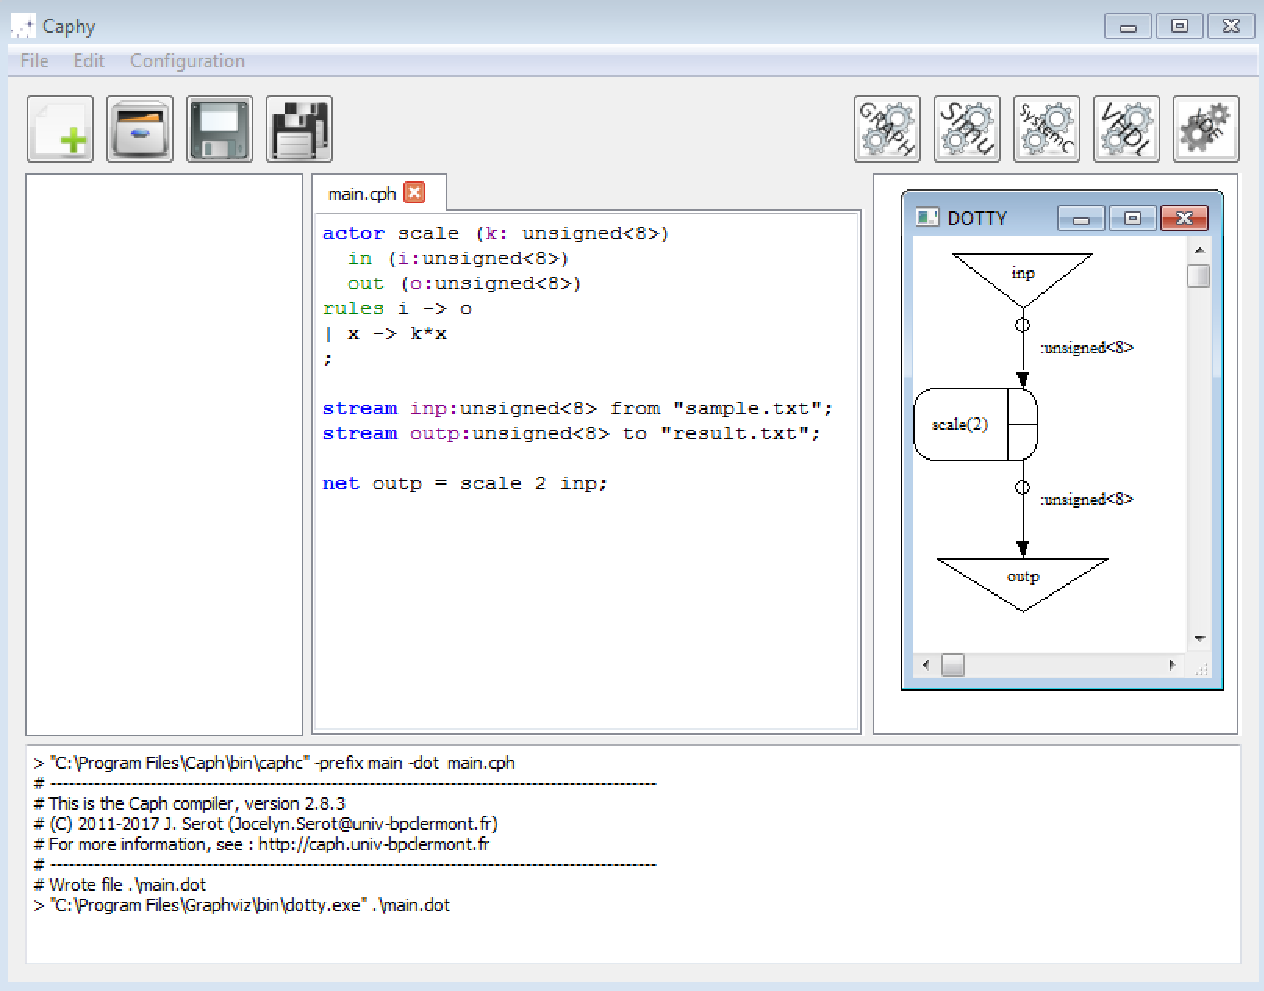
\includegraphics[width=0.75\textwidth]{figs/ide/make-dot}
  \caption{Viewing the dataflow graph of the program}
  \label{fig:make-dot}
\end{figure}

\medskip
For \textbf{simulating the program}, we first need to create the file \texttt{sample.txt} containing
the input tokens. Click on the \textsf{New File} button and type, for example, the following line in
the newly created file tab :

\begin{verbatim}
1 2 3 4
\end{verbatim}

Save the file under name \texttt{sample.txt} in the directory containing the caph source file (see
Fig.~\ref{fig:write-sample}).

\begin{figure}[h]
  \centering
  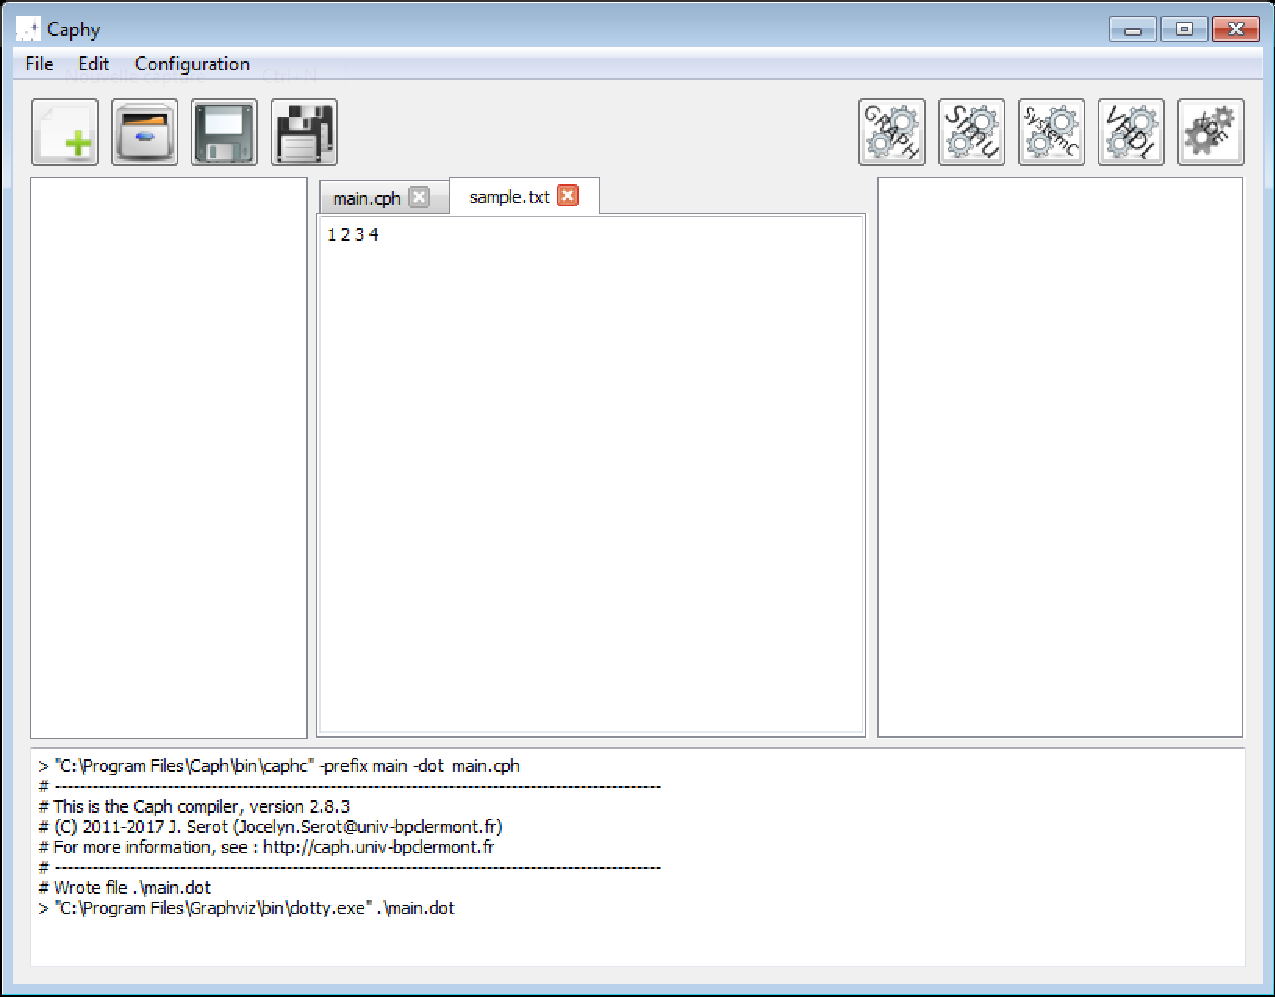
\includegraphics[width=0.75\textwidth]{figs/ide/write-sample}
  \caption{Writing the input data file for simulation}
  \label{fig:write-sample}
\end{figure}

Go back to the \caph source file by selecting the corresponding tab\footnote{Simulation will not
  work otherwise !}  and invoke the compiler by clicking on the \textsc{Simu} button. This will run
the program, generate results in the file \texttt{result.txt}\footnote{As specified by the
  \texttt{stream ... from} line in the program.} and display the latter in a separate tab, as shown
in Fig.~\ref{fig:make-sim}.

\begin{figure}[h]
  \centering
  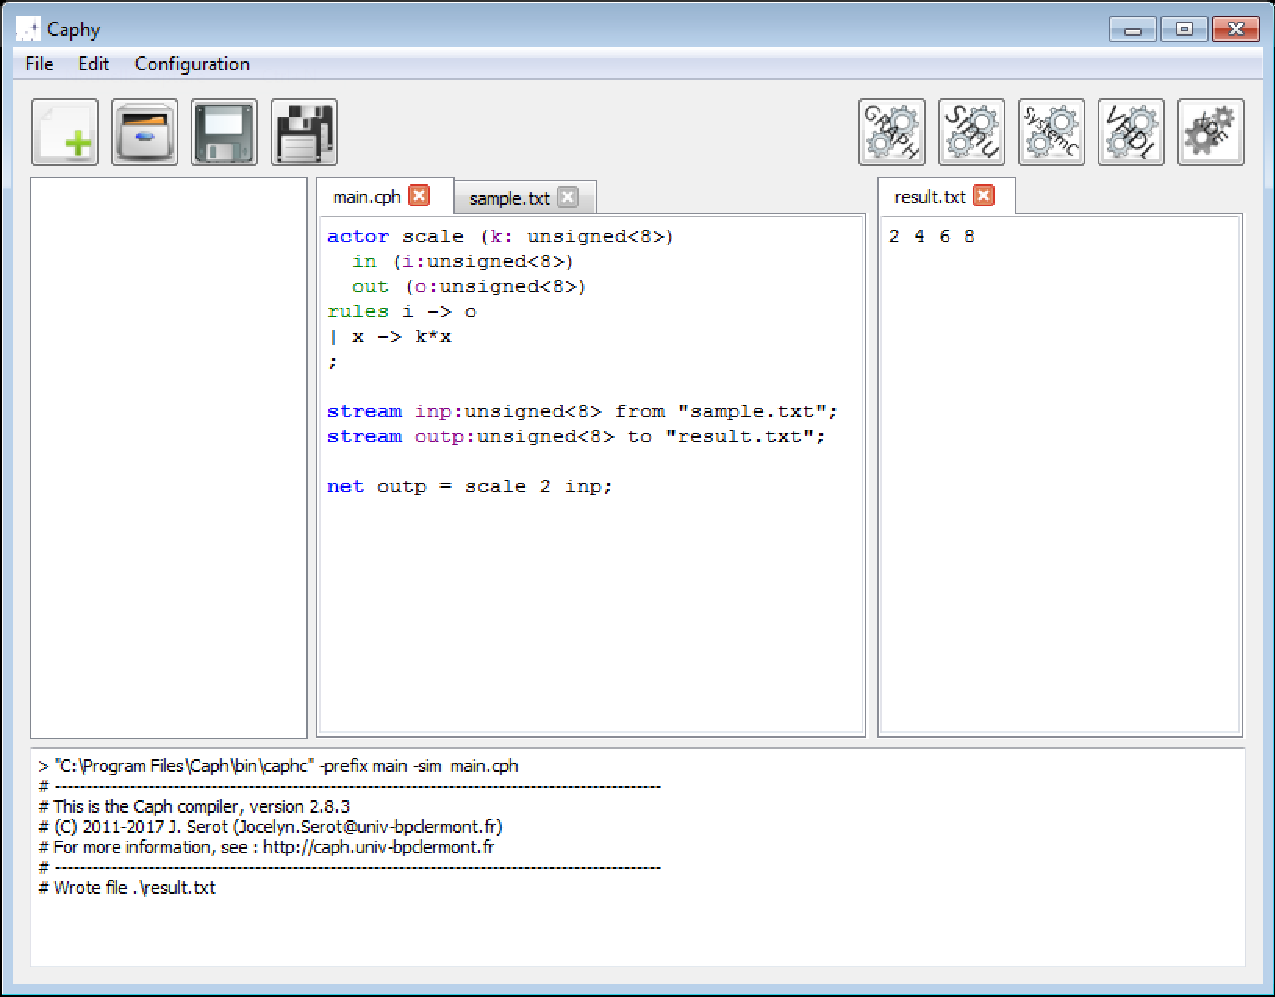
\includegraphics[width=0.75\textwidth]{figs/ide/make-sim}
  \caption{Viewing simulation results}
  \label{fig:make-sim}
\end{figure}

\medskip
For \textbf{generating the SystemC, VHDL or XDF} representation of the program, follow the procedure
described for generating the graph representation :
\begin{enumerate}
\item select the tab containing the source program
\item click on the \textsf{SystemC} (resp. \textsf{VHDL}, resp. \textsf{XDF}) button
\end{enumerate}
The result files will be generated in the same directory and displayed as separate tabs on the
right, as illustrated in figures.~\ref{fig:make-systemc} and \ref{fig:make-vhdl} respectively.

\begin{figure}[h]
  \centering
  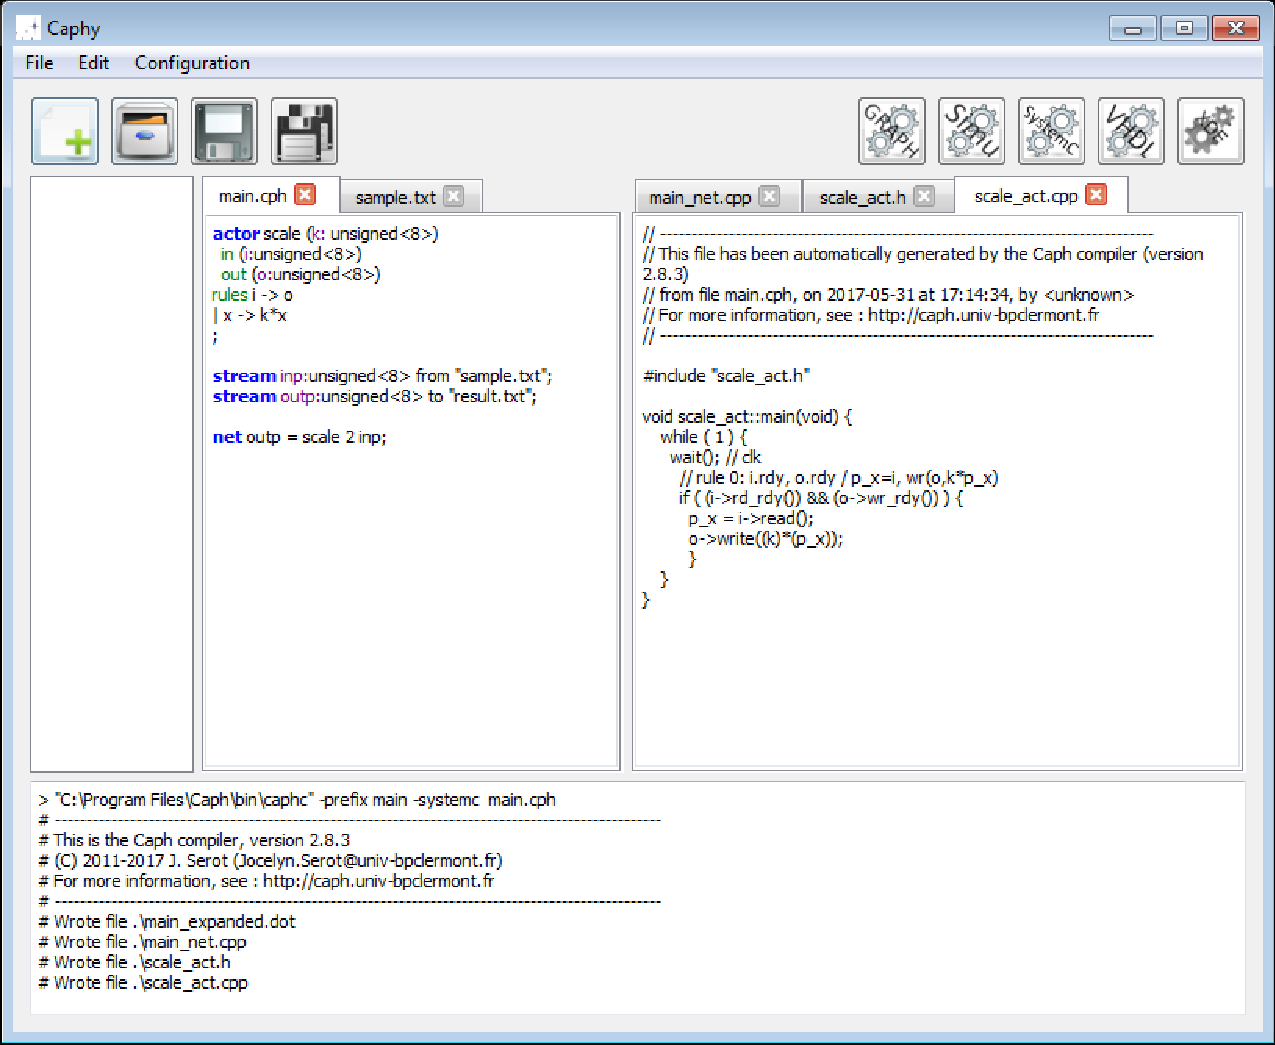
\includegraphics[width=0.75\textwidth]{figs/ide/make-systemc}
  \caption{After generating SystemC code}
  \label{fig:make-systemc}
\end{figure}

\begin{figure}[h]
  \centering
  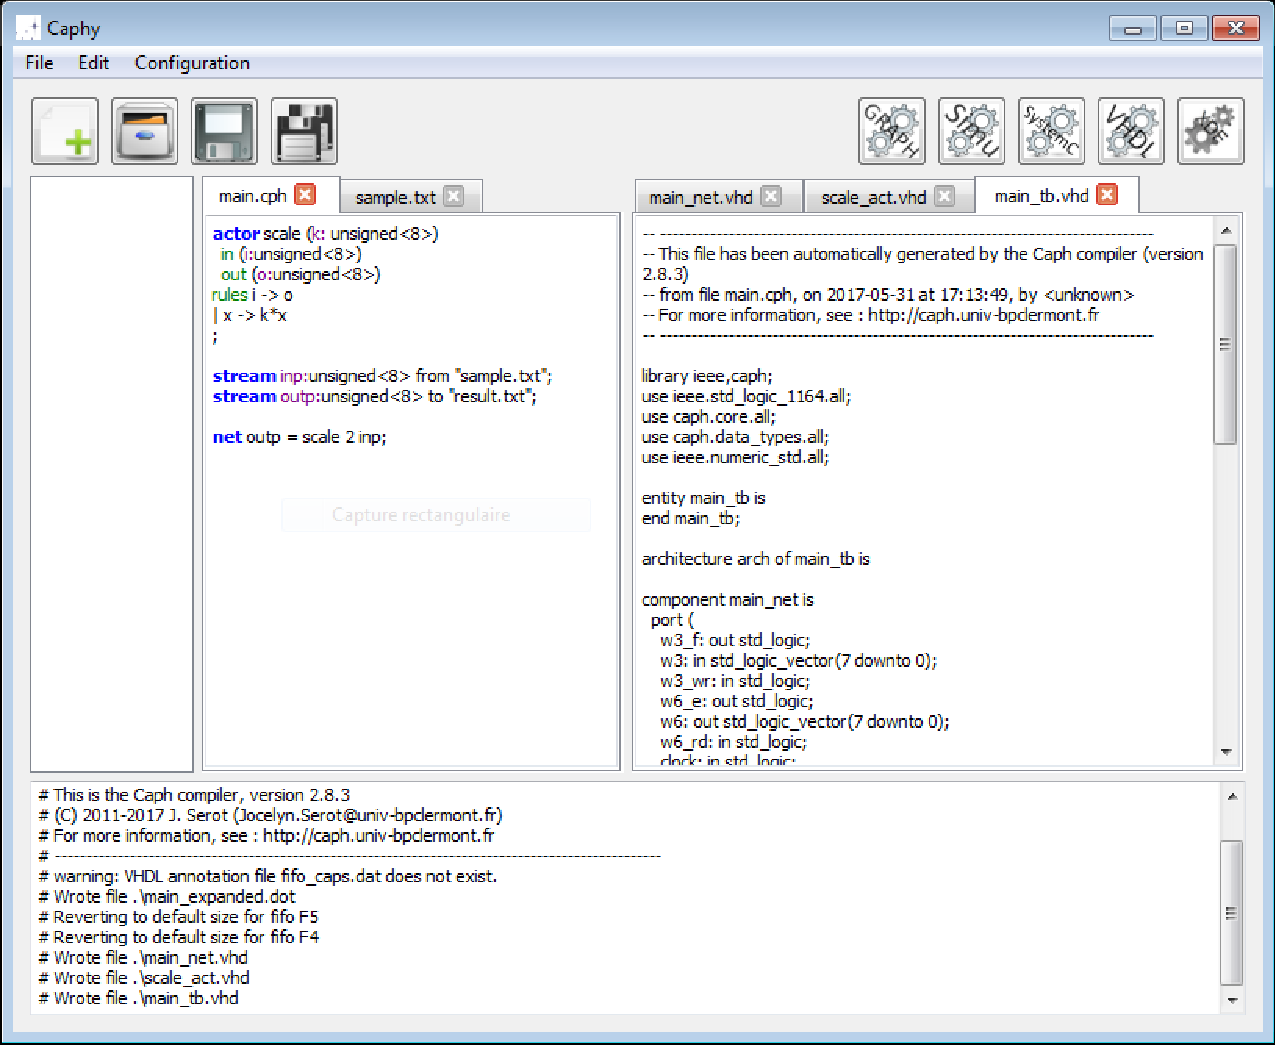
\includegraphics[width=0.75\textwidth]{figs/ide/make-vhdl}
  \caption{After generating VHDL code}
  \label{fig:make-vhdl}
\end{figure}

%%% Local Variables: 
%%% mode: latex
%%% TeX-master: "caph-primer"
%%% End: 

%%%%%%%%%%%%%%%%%%%%%%%%%%%%%%%%%%%%%%%%%%%%%%%%%%%%%%%%%%%%%%%%%%%%%%%%%%%%%%%%%%%%%%%%%
%%                                                                                     %%
%%                This file is part of the CAPH Compiler distribution                  %%
%%                            http:%/caph.univ-bpclermont.fr                           %%
%%                                                                                     %%
%%                                  Jocelyn SEROT                                      %%
%%                         Jocelyn.Serot@univ-bpclermont.fr                            %%
%%                                                                                     %%
%%         Copyright 2011-2018 Jocelyn SEROT.  All rights reserved.                    %%
%%  This file is distributed under the terms of the GNU Library General Public License %%
%%      with the special exception on linking described in file ..%LICENSE.            %%
%%                                                                                     %%
%%%%%%%%%%%%%%%%%%%%%%%%%%%%%%%%%%%%%%%%%%%%%%%%%%%%%%%%%%%%%%%%%%%%%%%%%%%%%%%%%%%%%%%%%

\chapter{Working with projects}
\label{cha:ide-project}

The \caph IDE provides a simple way of organizing files related to a given application within an entity
called a \emph{project}. Technically, a \emph{project} is nothing but a directory gathering all
files related to an application. This includes \caph source files, input data files for simulation,
files saving compiler options and a collection of subdirectories containing the files
produced by the compiler in graph, simulation, SystemC or VHDL mode. Having a separate directory for
each mode makes interfacing to external tools -- C++ compiler, VHDL simulators and synthetizers in
particular -- easier.

\medskip
In this chapter we will describe first how to create new projects and second how to use existing projects.

\section{Creating a project}
\label{sec:creating-project}

For simplicity, the created project will include a single source file, similar to that used
in chapter~\ref{cha:ide-basic}.

\medskip
\step \textbf{Create a new project} by invoking the corresponding item in the \textsf{File}
menu. In the displayed dialog (Fig.~\ref{fig:create-project}) give a a name to the project and
specify a directory to host it. For example, if the name is \texttt{myproj} and the root directory
\verb|C:\Users\Bob\Desktop|, then all the files related to the project will be stored in
directory \verb|C:\Users\Bob\Desktop\myproj|. If the projet needs additionnal, pre-existing
source or data files, add them in the corresponding text box or using the provided button. These
files will be automatically copied in the project directory. No additionnal file is needed here.

\begin{figure}[h]
  \centering
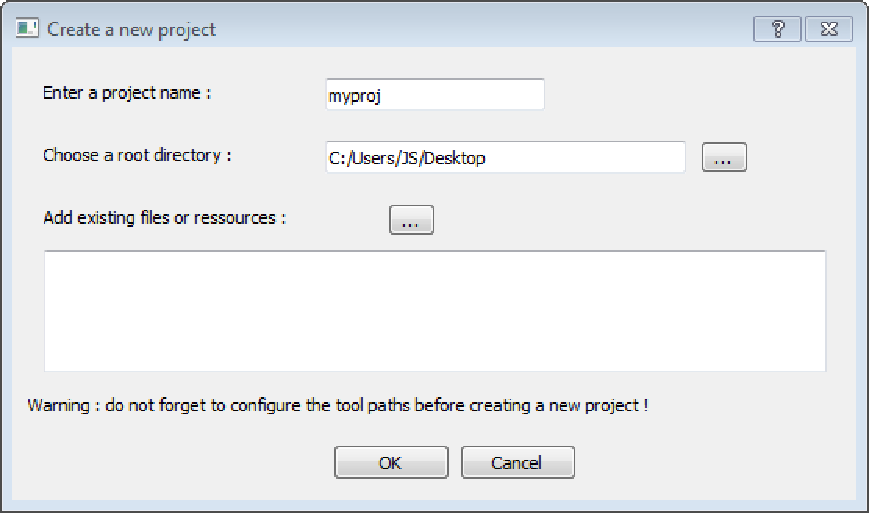
\includegraphics[width=0.75\textwidth]{figs/ide/create-project}
  \caption{The dialog shown when creating a new project}
  \label{fig:create-project}
\end{figure}

\step When a project \texttt{myproj} is created, a "main" source file is created with name
\texttt{main.cph} in the project directory and a file tab for editing is file is created (see
Fig.~\ref{fig:project-main}). Type the \caph source code of your program here\footnote{If you
  already have the source code, you can of course copy it and paste it.} and save it (see
Fig.~\ref{fig:project-main-done}). 

\begin{figure}[h]
  \centering
  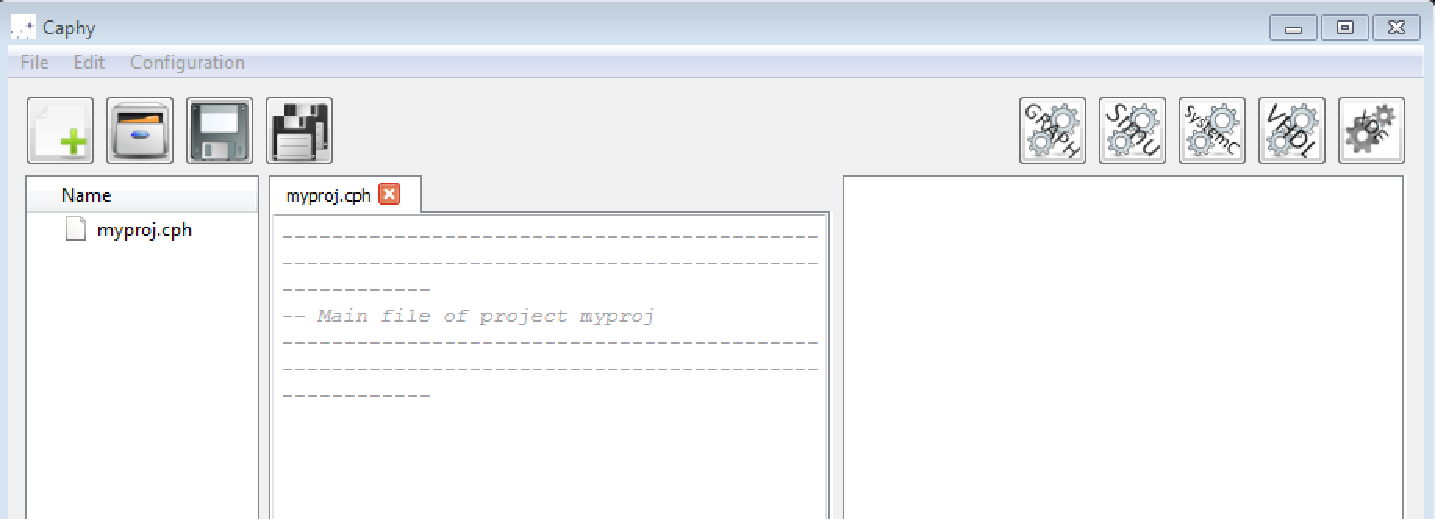
\includegraphics[width=0.75\textwidth]{figs/ide/project-main}
  \caption{Ready to edit the project main source file}
  \label{fig:project-main}
\end{figure}

\begin{figure}[h]
  \centering
  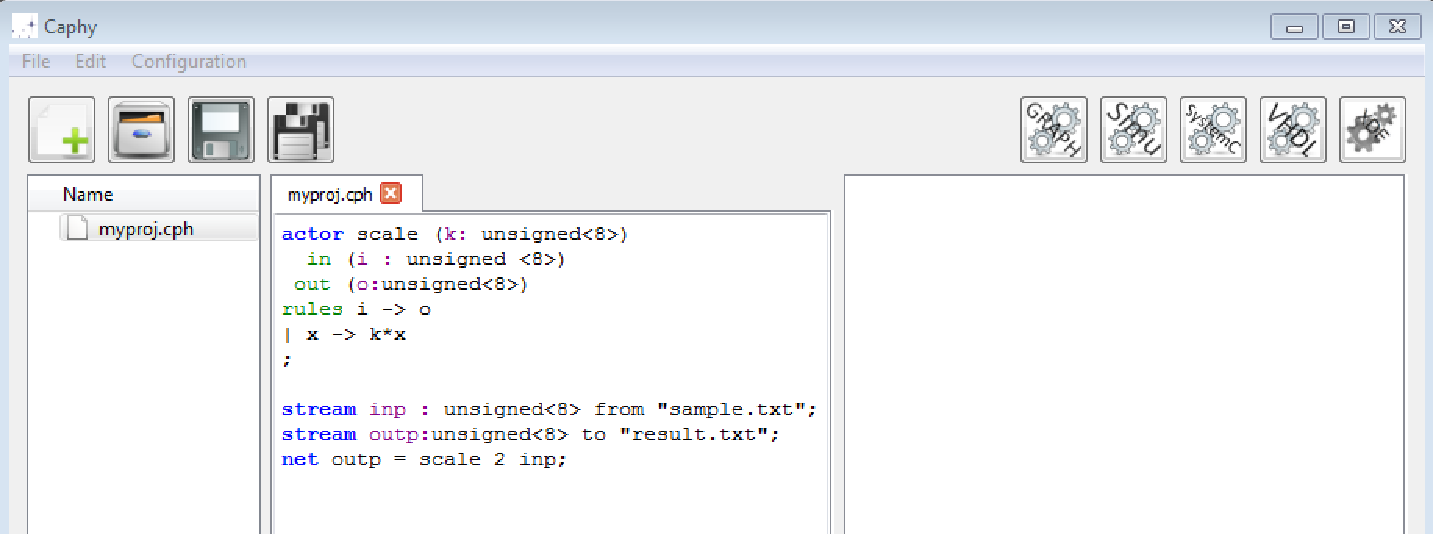
\includegraphics[width=0.75\textwidth]{figs/ide/project-main-done}
  \caption{Main source file completed}
  \label{fig:project-main-done}
\end{figure}

\medskip
\step From now, each compile action will 
\begin{itemize}
\item implicitely operate on the project main source file,
\item generate results in a specific directory (\texttt{dot} for graph, \texttt{simu} for
  simulation, \texttt{systemc}, \texttt{vhdl} and \texttt{xdf}).
\end{itemize}

The project tree representation (on the left) will be automatically updated to reflect the effect of
each compile action. Navigation within this tree  is of course allowed and double clicking on an
element will open the corresponding file in a distinct tab (if not already opened).

For example, Fig.~\ref{fig:project-make} display the GUI after clicking the \textsf{Graph}
and the \textsf{SystemC} compile buttons. The complete list of generated files for each step can be viewed by
clicking on the respective subdirectory in the tree view on the left.

\begin{figure}[h]
  \centering
  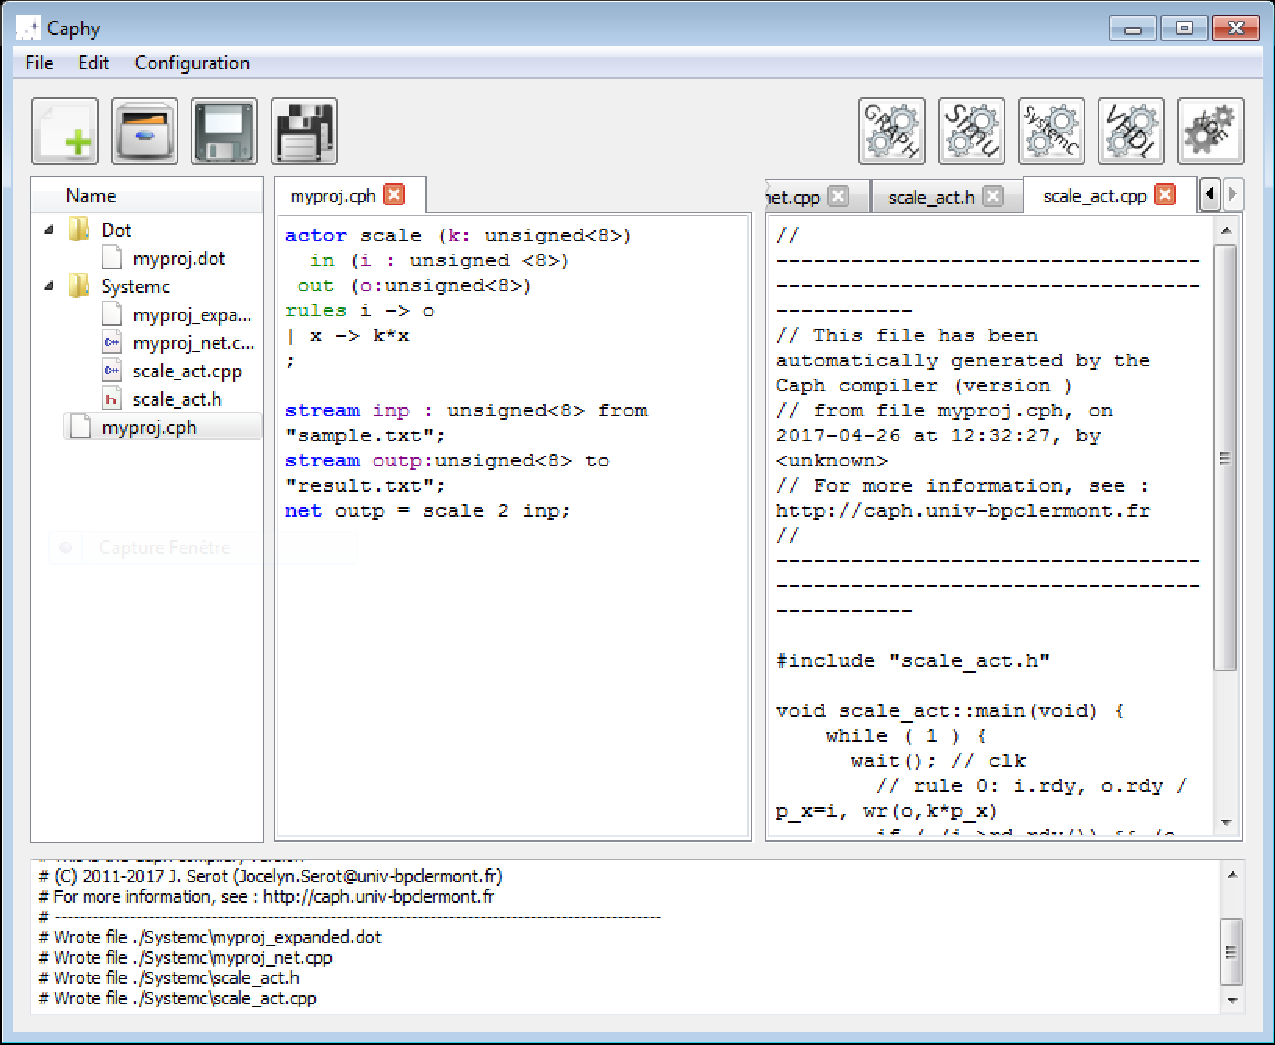
\includegraphics[width=0.75\textwidth]{figs/ide/project-make}
  \caption{After clicking the \textsf{Graph} and \textsf{SystemC} buttons in project mode}
  \label{fig:project-make}
\end{figure}

% \begin{figure}[h]
%   \centering
%   %\includegraphics[width=0.75\textwidth]{figs/first-launch}
%   \caption{After clicking the \textsf{SystemC} button in project mode}
%   \label{fig:project-make-sysc}
% \end{figure}

\section{Opening an existing project}
\label{sec:opening-a-project}

To open an existing projec, invoke the \textsf{Open Project} item of the
\textsf{File} menu and specify the name of the project description file (ending with the
\verb|.cphpro| extension), located in the project directory.

\medskip
For example, Fig.~\ref{fig:opening-primer-proj} shows the IDE
just about to open the project located in \texttt{primer/simple} directory which can be found in the
examples provided with the \caph distribution\footnote{These examples have here been installed in
  \texttt{Documents/CaphExamples}.}. This project corresponds to the program described in Part 1 of
this document. 

Fig.~\ref{fig:opened-primer-proj} shows the IDE just after opening this project.
 
\begin{figure}[h]
  \centering
  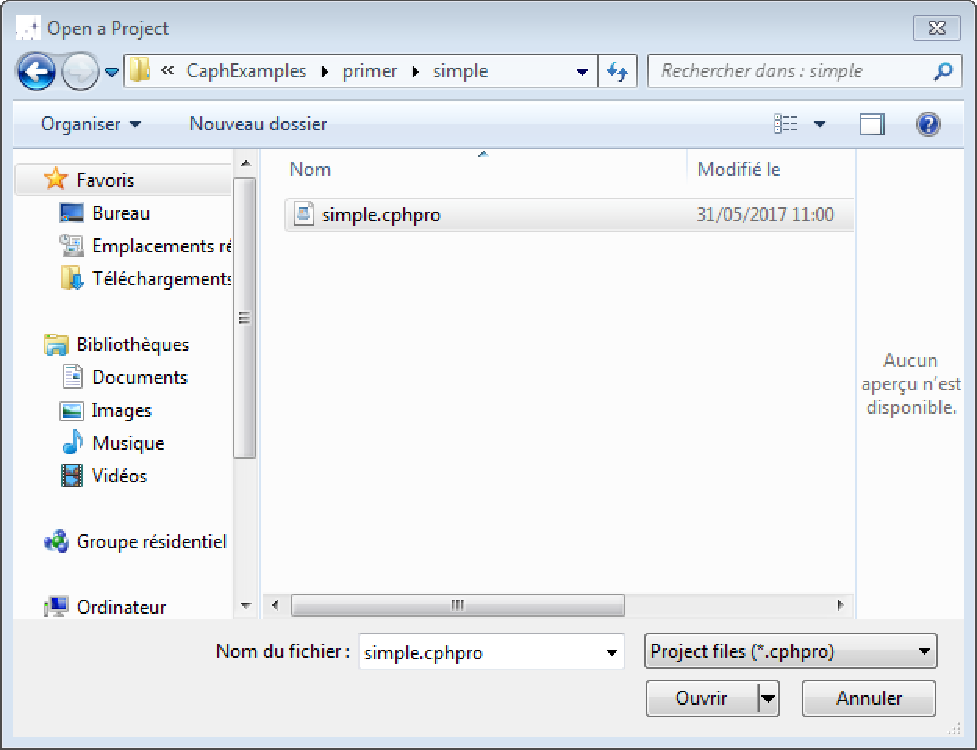
\includegraphics[width=0.75\textwidth]{figs/ide/opening-project}
  \caption{About to open the \texttt{Primer} project}
  \label{fig:opening-primer-proj}
\end{figure}

\begin{figure}[h]
  \centering
  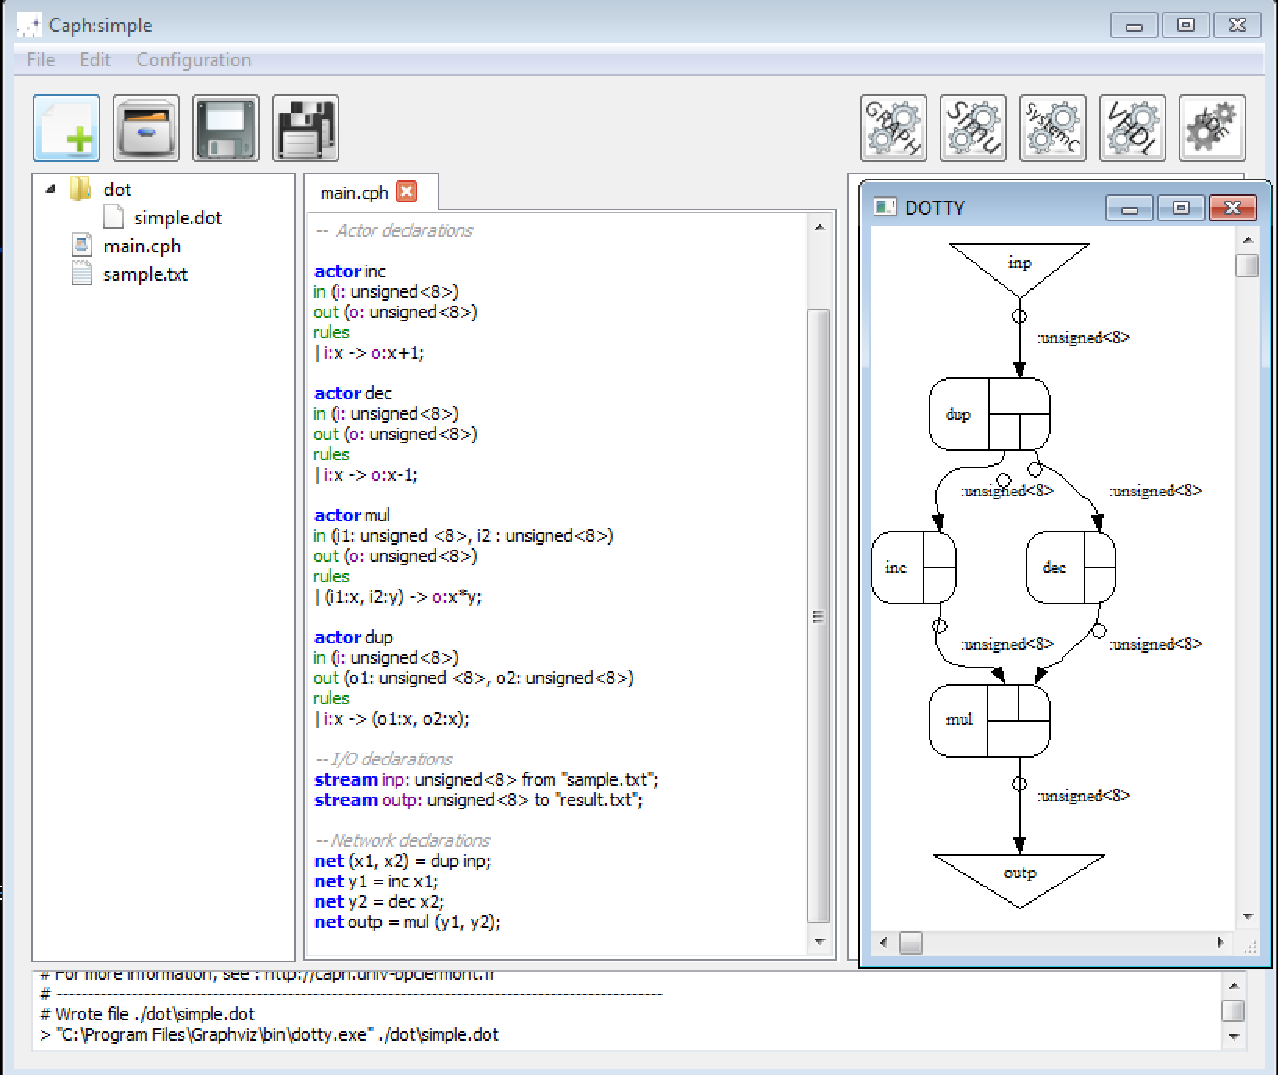
\includegraphics[width=0.95\textwidth]{figs/ide/opened-project}
  \caption{The \texttt{Primer} project opened}
  \label{fig:opened-primer-proj}
\end{figure}

%%% Local Variables: 
%%% mode: latex
%%% TeX-master: "caph-primer"
%%% End: 

%%%%%%%%%%%%%%%%%%%%%%%%%%%%%%%%%%%%%%%%%%%%%%%%%%%%%%%%%%%%%%%%%%%%%%%%%%%%%%%%%%%%%%%%%
%%                                                                                     %%
%%                This file is part of the CAPH Compiler distribution                  %%
%%                            http:%/caph.univ-bpclermont.fr                           %%
%%                                                                                     %%
%%                                  Jocelyn SEROT                                      %%
%%                         Jocelyn.Serot@univ-bpclermont.fr                            %%
%%                                                                                     %%
%%         Copyright 2011-2018 Jocelyn SEROT.  All rights reserved.                    %%
%%  This file is distributed under the terms of the GNU Library General Public License %%
%%      with the special exception on linking described in file ..%LICENSE.            %%
%%                                                                                     %%
%%%%%%%%%%%%%%%%%%%%%%%%%%%%%%%%%%%%%%%%%%%%%%%%%%%%%%%%%%%%%%%%%%%%%%%%%%%%%%%%%%%%%%%%%

\chapter{Compilation options}
\label{cha:ide-options}

The caph compiler comes with a fairly large number of options (see Sec. 12 of the language reference
manual). Most of these options can be set and inspected by invoking \textsf{Compilater options} item
of the \textsf{Configuration} menu. Options are organized by grouped by tabs, as illustrated in
Fig.~\ref{fig:options-sysc}, in which the tab related to SystemC has been selected.

\begin{figure}[h]
  \centering
  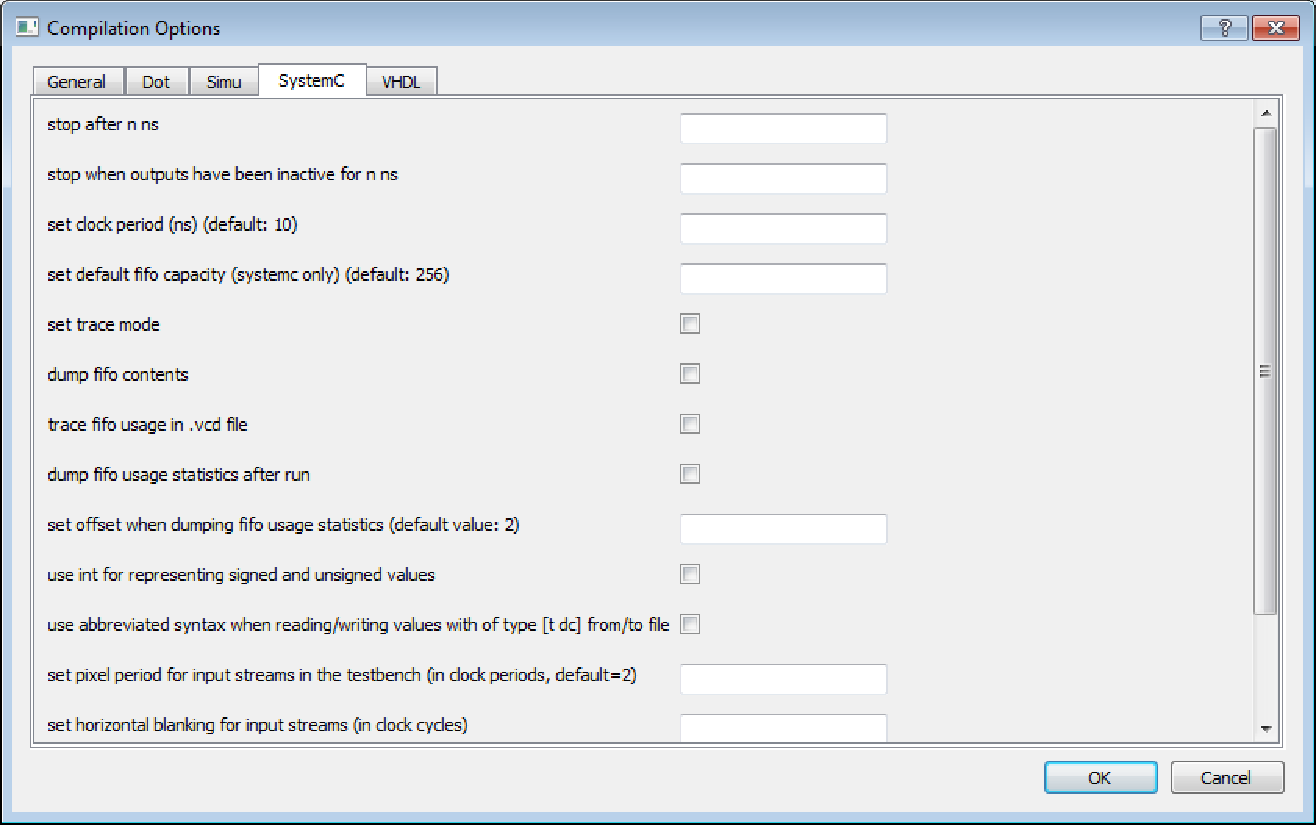
\includegraphics[width=0.75\textwidth]{figs/ide/options-sysc}
  \caption{The options setting dialog}
  \label{fig:options-sysc}
\end{figure}

\medskip An important point is that, when working in project mode, each modification to compilation
options is recorded and saved in a dedicated file in the project directory. This file, when present,
is automatically read when a project is opened. This way, compilation options are remembered between
sessions.

%%% Local Variables: 
%%% mode: latex
%%% TeX-master: "caph-primer"
%%% End: 

\part{Makefile-based design with Caph}
%%%%%%%%%%%%%%%%%%%%%%%%%%%%%%%%%%%%%%%%%%%%%%%%%%%%%%%%%%%%%%%%%%%%%%%%%%%%%%%%%%%%%%%%%
%%                                                                                     %%
%%                This file is part of the CAPH Compiler distribution                  %%
%%                            http:%/caph.univ-bpclermont.fr                           %%
%%                                                                                     %%
%%                                  Jocelyn SEROT                                      %%
%%                         Jocelyn.Serot@univ-bpclermont.fr                            %%
%%                                                                                     %%
%%         Copyright 2011-2018 Jocelyn SEROT.  All rights reserved.                    %%
%%  This file is distributed under the terms of the GNU Library General Public License %%
%%      with the special exception on linking described in file ..%LICENSE.            %%
%%                                                                                     %%
%%%%%%%%%%%%%%%%%%%%%%%%%%%%%%%%%%%%%%%%%%%%%%%%%%%%%%%%%%%%%%%%%%%%%%%%%%%%%%%%%%%%%%%%%

\chapter*{Introduction}
\label{sec:cl-intro}

This part describes how to use \caph in a command line based environment, using
\texttt{Makefile}s. On Unix-like platforms like Linux or MacOS, this is typically accomplished by
running the corresponding tools from within a command shell. On Windows, this can be done using Unix
emulation systems like MinGW~\cite{MinGW} or Cygwin~\cite{CygWin}.  As stated in the general
introduction, although this approach may appear a bit more complicated than the former at first
sight but it provides a way of integrating existing third-party tools, such as C++ compilers and
VHDL synthetizers, in a fully automatized design flow. 

\medskip This part assumes a basic familiarity with command line interfaces, shell programming
and \texttt{make}-based compilation flows. Aside, a knowledge in digital design (and of the VHDL
language) will help to appreciate the final products of the \caph toolset. Sections describing the
synthesis of VHDL code on FPGA requires a previous knowledge of the \textsc{altera}
Quartus~\textsc{ii} environment.

\bigskip
The following typographic conventions are followed :
\begin{itemize}
\item source code is written in gray-shaded boxes, like this :
\begin{lstlisting}[style=CaphStyle]
-- CAPH source code will appear here
\end{lstlisting}
\item \texttt{makefile}s are written in pink-shaded boxes, like this :
\begin{lstlisting}[style=MakeStyle]
-- Makefiles will appear like this
\end{lstlisting}
\item shell input (on the command line) is written like this (the character \verb|#| is the shell
  prompt) :
\begin{lstlisting}[style=BashInputStyle]
# command
\end{lstlisting}
\item shell output is written like this :
\begin{lstlisting}[style=BashOutputStyle]
shell output
\end{lstlisting}
\end{itemize}

%%% Local Variables: 
%%% mode: latex
%%% TeX-master: "caph-primer"
%%% End: 

%%%%%%%%%%%%%%%%%%%%%%%%%%%%%%%%%%%%%%%%%%%%%%%%%%%%%%%%%%%%%%%%%%%%%%%%%%%%%%%%%%%%%%%%%
%%                                                                                     %%
%%                This file is part of the CAPH Compiler distribution                  %%
%%                            http:%/caph.univ-bpclermont.fr                           %%
%%                                                                                     %%
%%                                  Jocelyn SEROT                                      %%
%%                         Jocelyn.Serot@univ-bpclermont.fr                            %%
%%                                                                                     %%
%%         Copyright 2011-2018 Jocelyn SEROT.  All rights reserved.                    %%
%%  This file is distributed under the terms of the GNU Library General Public License %%
%%      with the special exception on linking described in file ..%LICENSE.            %%
%%                                                                                     %%
%%%%%%%%%%%%%%%%%%%%%%%%%%%%%%%%%%%%%%%%%%%%%%%%%%%%%%%%%%%%%%%%%%%%%%%%%%%%%%%%%%%%%%%%%

\chapter{Using the \caphc compiler}
\label{cha:cl-basic}

In this chapter, we will show how to invoke to \caphc compiler from the command line in order to
\begin{itemize}
\item generate and view the dataflow graph corresponding to a program,
\item simulate this program,
\item generate SystemC and VHDL code.
\end{itemize}

The program used as example will be the one introduced in Part 1 and given in
Listing~\ref{lst:simple-full}. We assume that the corresponding source code has been placed in a
file named \verb|simple.cph|. 

\section{Configuring}
\label{sec:cl-conf}

Add a variable named \verb|CAPH|, pointing to the root of your local CAPH installation, to your
environment. For example (with a Bash shell) : 

\begin{lstlisting}[style=BashInputStyle]
# CAPH=/usr/local/caph; export CAPH
\end{lstlisting}

Add \verb|$CAPH/bin| to your \verb|$PATH| environment, so that CAPH commands can be found :

\begin{lstlisting}[style=BashInputStyle]
# PATH=$CAPH/bin:$PATH; export $PATH
\end{lstlisting}
%$

\section{Viewing the dataflow graph}
\label{sec:drawing-network}

From the directory containing the source file, type, from a shell, the following command :  

\begin{lstlisting}[style=BashInputStyle]
# caphc -dot simple.cph
\end{lstlisting}

Executing this command yields the following output 

\begin{lstlisting}[style=BashOutputStyle]
-------------------------------------------------------------------------------------------------
This is the Caph compiler, version 2.8.3
(C) 2011-2017 J. Serot (Jocelyn.Serot@univ-bpclermont.fr)
For more information, see : http://caph.univ-bpclermont.fr
-------------------------------------------------------------------------------------------------
Wrote file ./simple.dot
\end{lstlisting}

and produces the graphical representation of the program in file named
\verb|simple.dot|. This file is in the DOT format and can be visualized with the
\texttt{graphviz} suite of tools~\cite{Graphviz}. Under MacOS, launch the \texttt{Graphviz}
application and open the corresponding file\footnote{Alternatively, from a terminal, type
  \texttt{open -a Graphviz simple.dot}.}. Under Windows, use the \texttt{dotty} application.
The resulting graph is shown in Fig.~\ref{fig:simple-dot}. The four involved actors
can be readily recongnized. Wires are labeled with the types of the conveyed values (the type of
intermediate wires is automatically inferred by the compiler). Input and output wires are drawn as
triangles. Several options of the compiler allow the aspect of this graphical representation and the
amount of displayed informations to be adjusted.

\begin{figure}[htbp]
  \centering
 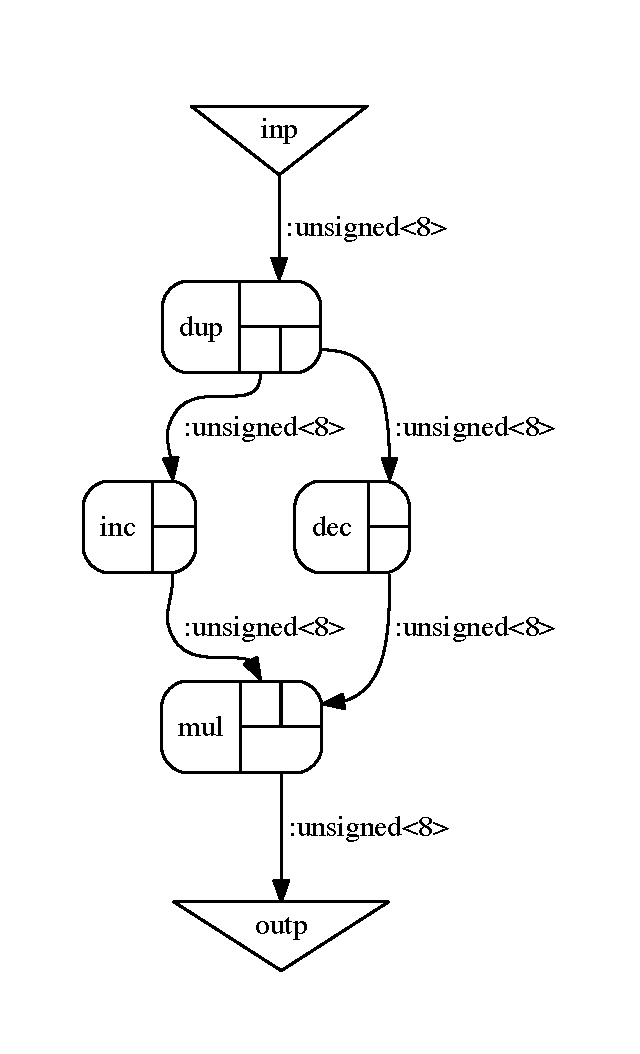
\includegraphics[width=0.3\textwidth]{./figs/simple-dot.pdf}
  \caption{The graphical representation of the program given in Listing.~\ref{lst:simple-full} computed
    by the \caph compiler front-end} 
  \label{fig:simple-dot}
\end{figure}

\section{Simulating the program}
\label{sec:simulation}

% Before generating the VHDL code, it is generally useful to simulate to program in order to check
% that it actually computes the expected results.

There are actually two ways of simulating programs : either directly from the source code, using the
reference interpreter of the language\footnote{As demonstrated in Part 2, with the IDE}, or by using
the SystemC backend.

In both cases, input(s) and output(s) will be read (resp. written) to text files\footnote{Of
  course, for the final application, running the on target hardware platform, there will have to be
  a builtin mechanism for producing the stream(s) of input tokens and consuming the stream(s) of
  output tokens. In practice, this mechanism will take the form of a couple 
  of dedicated VHDL processes reading and writing values from/to the I/O devices attached to the
  hardware platform (video cameras, digital display, host pc interface, \ldots).}.
Input text files can be simply written by hand or generated from other data representations (images,
in particulary) using ad-hoc conversion programs provided in the CAPH distribution (see Sec.~9.5 of
the reference manual). 

In our case, and in accordance to the
\verb|stream| declarations written in file \verb|simple.cph|, the input file will be named
\verb|sample.txt| and the output file \verb|result.txt|. The file \verb|sample.txt| simply contains
the sequence of input tokens (unsigned integers in this particular case, as shown in
Listing~\ref{lst:sample-input} :

\begin{lstlisting}[language=bash,frame=tb,caption={The input file \texttt{sample.txt} used for
    simulating the program of Listing~\ref{lst:simple-full}},label={lst:sample-input}]
1 2 3 4 5 6 7 8
\end{lstlisting}

\section{Simulation using the interpreter}
\label{sec:simul-using-interpr}

Simulation is launched by invoking the compiler with the \verb|-sim| option :

\begin{lstlisting}[style=BashInputStyle]
# caphc -sim simple.cph
\end{lstlisting}

Executing this command yields the following output 

\begin{lstlisting}[style=BashOutputStyle]
----------------------------------------------------------
This is the Caph compiler, version 2.8.3
...
Wrote file ./result.txt
----------------------------------------------------------
\end{lstlisting}

The contents of the file \verb|result.txt| is given in Listing~\ref{lst:sample-output}.

\begin{lstlisting}[language=bash,frame=tb,caption={The output file \texttt{result.txt} generated
    when simulating the program of Listing~\ref{lst:simple-full} with the input file of
    Listing~\ref{lst:sample-input}},label={lst:sample-output}]
0 3 8 15 24 35 48 63
\end{lstlisting}

\section{Simulation using the SystemC backend}
\label{sec:simul-using-syst}

This actually requires three steps : first generating the SystemC code representing the
application, second compiling this code to produce an executable and finally running this
executable.

The whole process is greatly simplified by using the \verb|caphmake| utility program included in
the distribution\footnote{Since version 2.8.1.}. This program automatically generates Makefile
descriptions from \emph{project} descriptions, describing the application-specific parameters. A
detailed presentation of \texttt{caphmake} can be found in Sec.~9.10 of the Reference Manual. We
will here only illustrate its basic usage.

\medskip Listing~\ref{lst:simple-proj-sysc} shows a very simple project file for compiling and
running the SystemC code derived from the \texttt{simple.cph} program. The \verb|SC_OPTS| macro
gives the options to pass the SystemC backend of the \texttt{caphc} compiler. 
Here the option \verb|-sc_stop_time| specifies the duration of the simulation in
\emph{ns}\footnote{The complete list of options is given in the language reference manual.}.

\begin{lstlisting}[style=MakeStyle,caption={File
    \texttt{simple.proj} for compiling and running SystemC code},label={lst:simple-proj-sysc}]
SC_OPTS = -sc_stop_time 200
\end{lstlisting}

\medskip
After writing \verb|simple.proj|, just invoke \texttt{caphmake} with the name of the main source
file :

\begin{lstlisting}[style=BashInputStyle]
# caphmake -main simple
\end{lstlisting}

This will write a file named \texttt{Makefile} in the current directory.

\medskip
Now use this top-level Makefile to generate the SystemC-specific makefile :

\begin{lstlisting}[style=BashInputStyle]
# make systemc.makefile
\end{lstlisting}

This will write a file named \texttt{Makefile.systemc} in the current directory.

\medskip
We now can generate the SystemC code by simply typing 

\begin{lstlisting}[style=BashInputStyle]
# make systemc.code
\end{lstlisting}

yielding the following output  

\begin{lstlisting}[style=BashOutputStyle,numbers=left,numberstyle=\tiny]
make -f Makefile.systemc code CAPH=/usr/local/caph
/usr/local/caph/bin/caphc -I /usr/local/caph/lib/caph -systemc -sc_stop_time 200 simple.cph
-------------------------------------------------------------------------------------------------
This is the Caph compiler, version 2.8.3
(C) 2011-2017 J. Serot (Jocelyn.Serot@univ-bpclermont.fr)
For more information, see : http://caph.univ-bpclermont.fr
-------------------------------------------------------------------------------------------------
Wrote file ./simple_expanded.dot
Wrote file ./simple_net.cpp
Wrote file ./dup_act.h
Wrote file ./dup_act.cpp
Wrote file ./mul_act.h
Wrote file ./mul_act.cpp
Wrote file ./dec_act.h
Wrote file ./dec_act.cpp
Wrote file ./inc_act.h
Wrote file ./inc_act.cpp
\end{lstlisting}

Line 2 shows the invocation of the \caph compiler with the SystemC backend.
Lines 8--17 show the different files generated by the \caph compiler. The file
\verb|simple_expanded.dot| is a variant of the file \verb|simple.dot| discussed in
Sec.~\ref{sec:drawing-network}\footnote{This variant, only required by the SystemC and VHDL backend,
  has explicit FIFO and flow-splitting nodes.}.  The file \texttt{simple\_net.cpp} contains the
top-level network description. The files \verb|dup_act.h| and \verb|dup_act.cpp| (resp. \verb|mul_act.h| and
  \verb|mul_act.cpp|, \verb|dec_act.h| and \verb|dec_act.cpp|, \verb|inc_act.h| and \verb|inc_act.cpp|)
  contain the interface and the implementation of the \verb|dup| (resp. \texttt{mul},
  \texttt{dec} and \texttt{inc}) actor.

\medskip
The generated code can be compiled by simply typing 

\begin{lstlisting}[style=BashInputStyle]
# make systemc.exe
\end{lstlisting}

yielding the following output, which shows the compilation of this code using the classical SystemC
flow (in our case, \verb|gcc|, with link to the \verb|systemc| library\footnote{Appropriate
  definitions are provided in the file \texttt{\$CAPH/lib/etc/Makefile.core} and can be adjusted according to your
  local SystemC installation.}).

\begin{lstlisting}[style=BashOutputStyle,numbers=left,numberstyle=\tiny]
make -f Makefile.systemc exe CAPH=/usr/local/caph
(cd .; g++ -std=c++11 -I. -I/usr/local/caph/lib/systemc -I/usr/local/systemc-2.3.1/include
  -Wno-deprecated -Wno-parentheses-equality -D_CPP11  -c `basename inc_act.cpp`)
(cd .; g++ -std=c++11 -I. -I/usr/local/caph/lib/systemc -I/usr/local/systemc-2.3.1/include
  -Wno-deprecated -Wno-parentheses-equality -D_CPP11  -c `basename dec_act.cpp`)
(cd .; g++ -std=c++11 -I. -I/usr/local/caph/lib/systemc -I/usr/local/systemc-2.3.1/include 
  -Wno-deprecated -Wno-parentheses-equality -D_CPP11  -c `basename mul_act.cpp`)
(cd .; g++ -std=c++11 -I. -I/usr/local/caph/lib/systemc -I/usr/local/systemc-2.3.1/include 
  -Wno-deprecated -Wno-parentheses-equality -D_CPP11  -c `basename dup_act.cpp`)
(cd .; g++ -std=c++11 -I. -I/usr/local/caph/lib/systemc -I/usr/local/systemc-2.3.1/include 
  -Wno-deprecated -Wno-parentheses-equality -D_CPP11  -c `basename simple_net.cpp`)
(cd .; g++ -L/usr/local/systemc-2.3.1/lib-macosx64 inc_act.o dec_act.o mul_act.o dup_act.o simple_net.o
   -o simple_sc -lsystemc  2>&1 | c++filt)
\end{lstlisting}

\medskip
Finally, simulation is launched by running the compiled executable

\begin{lstlisting}[style=BashInputStyle]
# make systemc.run
\end{lstlisting}

yielding the following output 

\begin{lstlisting}[style=BashOutputStyle,numbers=left,numberstyle=\tiny]
make -f Makefile.systemc run CAPH=/usr/local/caph
./simple_sc

        SystemC 2.3.1-Accellera --- Aug  9 2015 15:42:56
        Copyright (c) 1996-2014 by all Contributors,
        ALL RIGHTS RESERVED
Simulation stopped at t=200 ns
Wrote file result.txt
\end{lstlisting}

The generated file \verb|result.txt| contains the results of the simulation (which is exactly the
same as the one obtained when running the source level simulator).

\medskip
The three different steps (code generation, compilation, execution) can be run with a simple command
by simply typing \verb|make systemc.run| directly after invoking \verb|caphmake|.

\section{Generating and  simulating VHDL code}
\label{sec:generating-vhdl}

The \caph compiler can produce a complete RT-level VHDL representation of the application which can
be simulated and, latter synthetised using vendor specific tools (such as \textsc{altera} Quartus or
\textsc{xilinx} ISE). This section focuses on simulation (synthesis will be covered in
Sec.~\ref{sec:synth-vhdl-code}). 

\medskip
Classicaly, simulation of VHDL code is performed using dedicated simulators included in the vendor
toolsets (for example, the ALTERA Quartus toolset includes the \texttt{modelsim} simulator). We
describe here another approach, using a freely available VDHL compiler and simulator called
GHDL~\cite{GHDL}. GHDL can be invoked directly from the command line and hence can be easily
integrated in a makefile-based design-flow.

\medskip As for the SystemC backend, the \textbf{first step} is to define, in the project
description file (\verb|.proj|), all the application-specific options. In our case, the only thing
to do is add a line dedicated to the VHDL backend in the file described in
Listing~\ref{lst:simple-proj-sysc}, as shown in Listing~\ref{lst:simple-proj-vhdl}. 

\begin{lstlisting}[style=MakeStyle,caption={File
    \texttt{simple.proj} for compiling and running SystemC and VHDL code},label={lst:simple-proj-vhdl}]
SC_OPTS = -sc_stop_time 200
GHDL_RUN_OPTS = --stop-time=200ns
\end{lstlisting}

The added line (line 2) specifies to options to be passed to the GHDL simulator. 

\medskip
After that, the process is very similar to that described in the previous section for the SystemC
backend :

\begin{itemize}
\item invoke \verb|make vhdl.makefile| to build the VHDL-specific \textrm{Makefile},
\item invoke \verb|make vhdl.code| to generate the VHDL code,
\item invoke \verb|make vhdl.exe| to build the executable,
\item invoke \verb|make vhdlrunexe| to run the simulation.
\end{itemize}

As before, the three last steps can be obtained by simply typing 

\begin{lstlisting}[style=BashInputStyle]
# make vhdl.run
\end{lstlisting}

yielding, in our case, the following output 

\begin{lstlisting}[style=BashOutputStyle,numbers=left,numberstyle=\tiny]
make -f Makefile.vhdl run CAPH=/usr/local/caph
/usr/local/caph/bin/caphc -I /usr/local/caph/lib/caph -vhdl  simple.cph
-------------------------------------------------------------------------------------------------
This is the Caph compiler, version 2.8.3
(C) 2011-2017 J. Serot (Jocelyn.Serot@univ-bpclermont.fr)
For more information, see : http://caph.univ-bpclermont.fr
-------------------------------------------------------------------------------------------------
Wrote file ./simple_expanded.dot
Reverting to default size for fifo F12
Reverting to default size for fifo F11
Reverting to default size for fifo F10
Reverting to default size for fifo F9
Reverting to default size for fifo F8
Reverting to default size for fifo F7
Wrote file ./simple_net.vhd
Wrote file ./dup_act.vhd
Wrote file ./mul_act.vhd
Wrote file ./dec_act.vhd
Wrote file ./inc_act.vhd
Wrote file ./simple_tb.vhd
warning: VHDL annotation file fifo_caps.dat does not exist.
(cd .; ghdl -a -P/usr/local/caph/lib/vhdl `basename simple_tb.vhd`)
(cd .; ghdl -a -P/usr/local/caph/lib/vhdl `basename inc_act.vhd`)
(cd .; ghdl -a -P/usr/local/caph/lib/vhdl `basename dec_act.vhd`)
(cd .; ghdl -a -P/usr/local/caph/lib/vhdl `basename mul_act.vhd`)
(cd .; ghdl -a -P/usr/local/caph/lib/vhdl `basename dup_act.vhd`)
(cd .; ghdl -a -P/usr/local/caph/lib/vhdl `basename simple_net.vhd`)
(cd .; ghdl -e -P/usr/local/caph/lib/vhdl simple_tb)
/usr/local/caph/bin/txt2bin uint 8 sample.txt > sample.bin
ghdl -r -P/usr/local/caph/lib/vhdl simple_tb --stop-time=200ns --vcd=simple_tb.vcd 
./simple_tb:info: simulation stopped by --stop-time
\end{lstlisting}

Line 2 shows the invocation of the \caph compiler with the VHDL backend. The produced files are
listed on lines 15--20. The file \texttt{simple\_net.vhd} contains the top-level network
description, The files \verb|{dup_act.vhd|, \verb|mul_act.vhd|, \verb|dec_act.vhd| and
  \verb|inc_act.vhd| contain the RTL description of the actors involved in this network. The file
  \verb|simple_tb.vhd| contains a testbench for performing the simulation at the RTL
  level. Simulation itself is performed as shown in line 30.

  Line 29 shows the invocation of the \verb|txt2bin| utility program to generate the file
  \verb|sample.bin| to be used as input for simulation. The reason for this is that the input data
  files read by the VHDL code use a special, text-encoded binary format. The \verb|txt2bin| program
  is used to convert the input simulation file \verb|sample.txt| to this format\footnote{The extra
    arguments to the program, \texttt{uint 8} in this case, are infered from the type of the
    corresponding input stream. A complete description of the binary format and the associated
    converter programs is provided in the reference manual.}.

Simulation results are produced in file \verb|result.bin|. This file is encoded using the same
binary format and can be decoded using the \verb|bin2txt| utility program. For this, it suffices to
invoke 

\begin{lstlisting}[style=BashInputStyle]
# make vhdl.show
\end{lstlisting}

This yields the following result, which shows the expected values in file \texttt{result.txt}

\begin{lstlisting}[style=BashOutputStyle,numbers=left,numberstyle=\tiny]
make -f Makefile.vhdl show CAPH=/usr/local/caph
/usr/local/caph/bin/bin2txt uint 8 result.bin > result.txt
result.txt: 0 3 8 15 24 35 48 63 
\end{lstlisting}

\medskip
The ``functional'' style of simulation illustrated above is in general sufficient for assessing the
code. It is however possible to get a more ``time oriented'' view by using the \verb|--vcd| option
of the GHDL compiler. This option must be added to the macro \verb|GHDL_RUN_OPTS| in the project
file, as shown in Listing~\ref{lst:simple-proj-vhdl2}.

\begin{lstlisting}[style=MakeStyle,caption={File
    \texttt{simple.proj} for compiling and running SystemC and VHDL code (2nd
    version)},label={lst:simple-proj-vhdl2}]
SC_OPTS = -sc_stop_time 200
GHDL_RUN_OPTS = --stop-time=200ns --vcd=simple_tb.vcd
\end{lstlisting}

This instructs the GHDL simulator to dump a detailed \emph{log} of the simulation in VCD
format~\cite{VCD}. This log file can examined using various waveform visualisation
programs. Fig.~\ref{fig:simple-waves}, for example, shows an excerpt of the log file as visualized
by the \verb|gtkwave| application~\cite{gtkwave}. Visualisation has been here limited to signals
connected to the instance of the \verb|inc| actor. One immediately spots the \verb|clock| and
\verb|reset| signals\footnote{The clock period is set by default to 10 ns. There's an option of the
  compiler to change it (see~\cite{caph-lrm}.}.  The signal \verb|i_empty| goes to 0 when a data is
available on the FIFO connected to input \verb|i| of the actor. Reading from the FIFO is then
triggered by setting signal \verb|i_rd| to 1. Symetrically, the signal \verb|o_full| is 0 when place
is available on the FIFO connected to output \verb|o| of the actor. Writing to this FIFO is then
triggered by setting signal \verb|i_wr| to 1.

\begin{figure}[htbp]
  \centering
 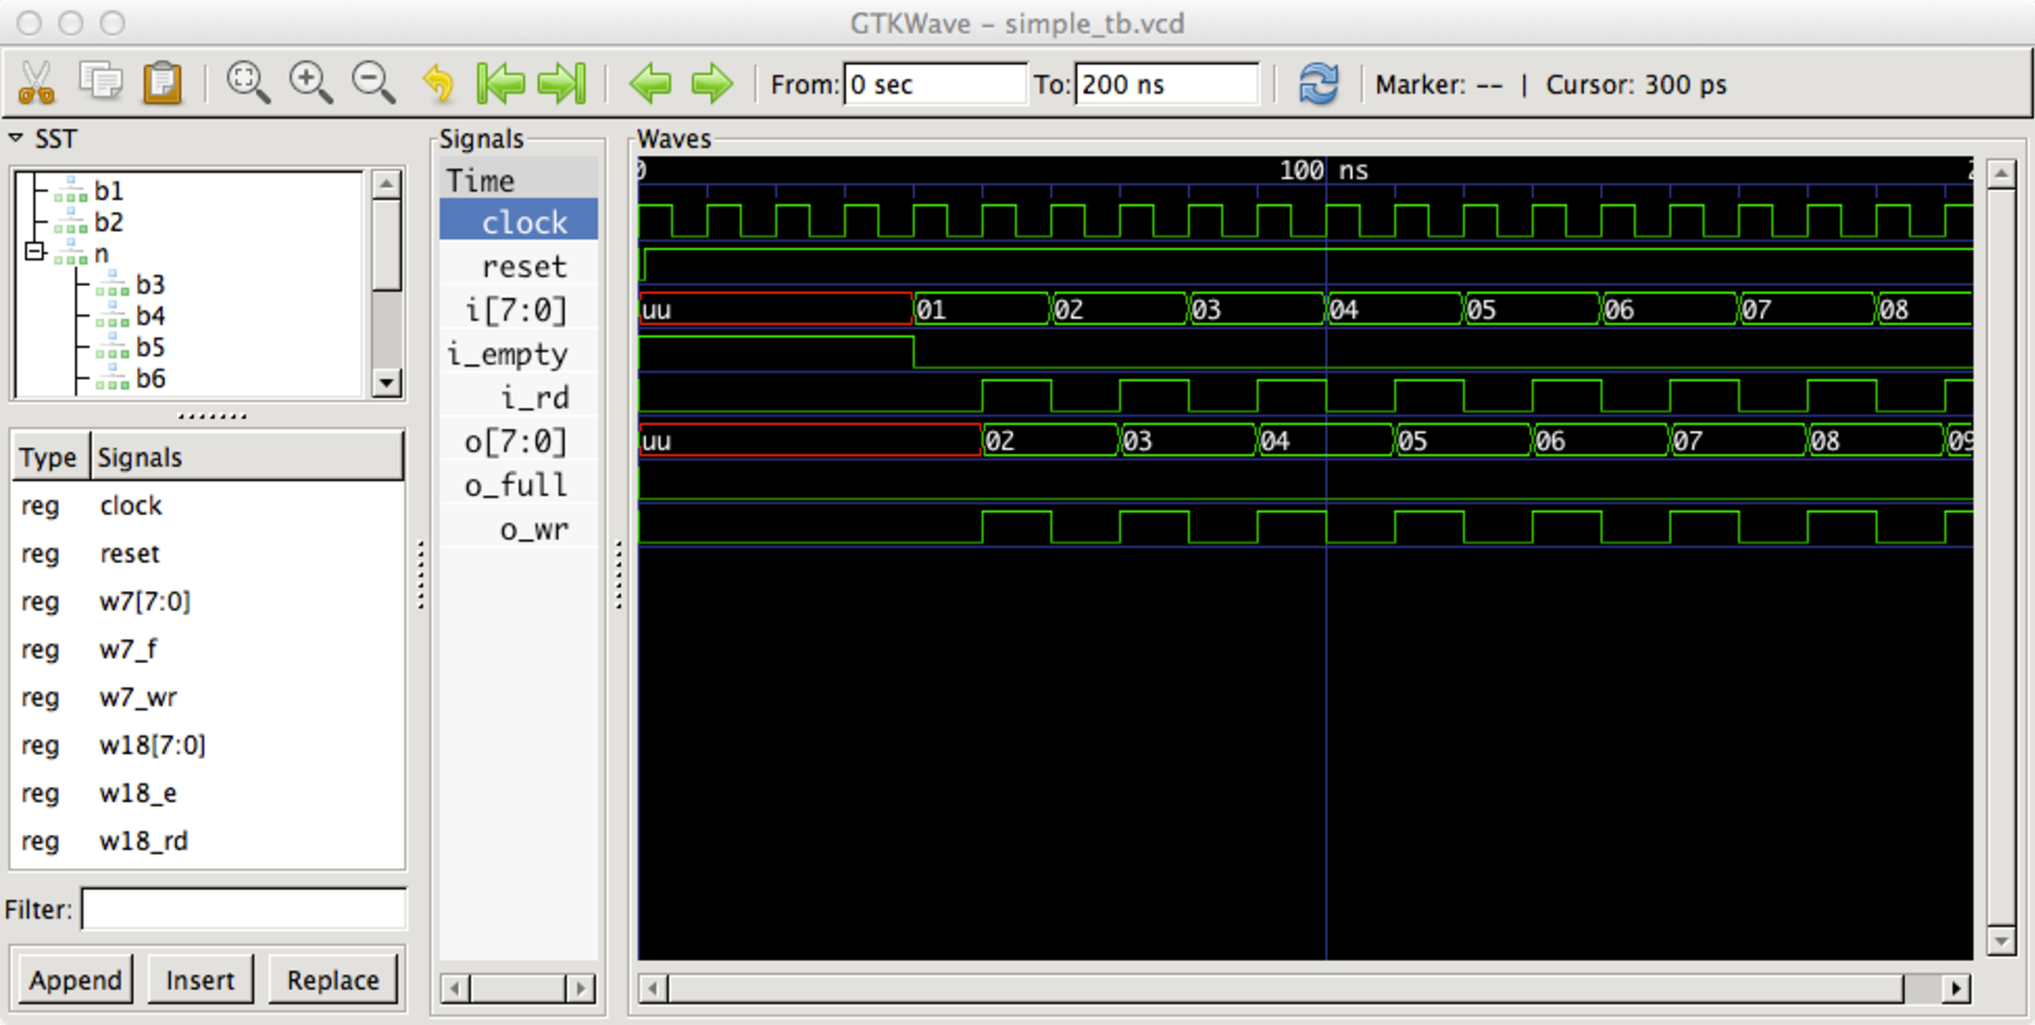
\includegraphics[width=\textwidth]{./figs/simple-waves.pdf}
  \caption{Some VHDL simulation results as viewed by \texttt{gtkwave}} 
  \label{fig:simple-waves}
\end{figure}

\section{Synthetizing the VHDL code}
\label{sec:synth-vhdl-code}

By synthesis we mean the tranformation of the RT-level code generated by the \caph compiler into a
FPGA configuration. Contrary to simulation, this operation depends on the physical target device and
requires the toolset from the corresponding vendor.  We do not address the issue of physical I/O
interfacing -- \emph{i.e.} we only describe the synthesis of the ``core'' functionality described by
the CAPH network (integration of CAPH-generated code into a full-fledged hardware platform is can be
carried out with the \textsc{GpStudio} IDE by example~\cite{GpStudio}).

In this section, we will illustrate the process
with the Quartus II suite of tools from \textsc{altera}, using the \verb|simple| application\footnote{This is
  only for pedagogical reasons since this application is obviously not a very useful one.
  Chap.\ref{cha:cl-images} and \ref{cha:cl-ip} will show how to implement more ``realistic'' applications,
  performing image processing.}.

\medskip Figs.\ref{fig:simple-quartus-1} to \ref{fig:simple-quartus-4} illustrates the creation of
the relevant project under the Quartus II (version 13.1) environment\footnote{We make the assumption
  here that the reader has a minimum familiarity with this environment. Several good tutorials can
  be found online, in particular on the ALTERA website.}.

Fig.~\ref{fig:simple-quartus-1} shows the
main Quartus window just after launching. In this window, select \textsf{File} in the top menu bar and
then the \textsf{New Project Wizard} item.

A window named after this item pops up. Fill the requested text
fields as illustrated in Fig.~\ref{fig:simple-quartus-2}. In our case, we have copied all the VHDL
files generated by the \caph compiler in a separate directory named
\verb|Z:/vhdl/caph/simple|\footnote{The option \texttt{-vhdl\_target\_dir} of the compiler can be
  used for that purpose.}. The
name of the project and the name of the top-level design entity must be set to
\verb|simple_net|. Clicking on the \textsf{Next} butten then brings the window shown in
Fig.~\ref{fig:simple-quartus-3}.

In this window, using the \textsf{...} and \textsf{Add} buttons, you have to specify the list of all the
VHDL files included in the projet. In our case, two groups of files are added : the five files
generated by the \caph compiler : \verb|dup_act.vhd|, \verb|mul_act.vhd|, \verb|dec_act.vhd|,
  \verb|inc_act.vhd| and \verb|simple_tb.vhd|; and two predefined files taken from the \caph VHDL
  library : \verb|../lib/caph.vhd| and \verb|../lib/fifo_fb.vhd| (the former contains a set of types
  and functions related to the \caph language, the latter the implementation of a generic
  FIFO). When completed, click again on the \textsf{Next} button.

  This brings up the window shown in Fig.~\ref{fig:simple-quartus-4}, in which you select the target
  device. In our case, a simple Cyclone III is chosen. Clicking then on the \textsf{Finish} button
  brings back to main window.

  On the \textsf{Project Navigator} subwindow (top left), select \textsf{Hierarchy} to show the design
  hierarchy. Selecting an entity will then print the corresponding source file on the right
  subwindow, as illustrated in Fig.~\ref{fig:simple-quartus-5}.

Synthesis is launched by selecting the \textsf{Start Compilation} item in the \textsf{Processing} menu
(or simply by clicking the small right-oriented purple triangle in the toolbar). Depending on your
machine this may take from a few seconds to a few minutes. In our case, the result is shown in
Fig.~\ref{fig:simple-quartus-6}. Here, it can be noted that only a very small fraction of the
available hardware resources is used.  

Fig.~\ref{fig:simple-quartus-7} shows the RT-level view of the design after
synthesis\footnote{Before physical mapping. It is also possible to get a post-mapping view.}. This
is obtained by invoking the \textsf{Netlist viewer} item in the \textsf{Tools} menu.

\begin{figure}[htbp]
  \centering
 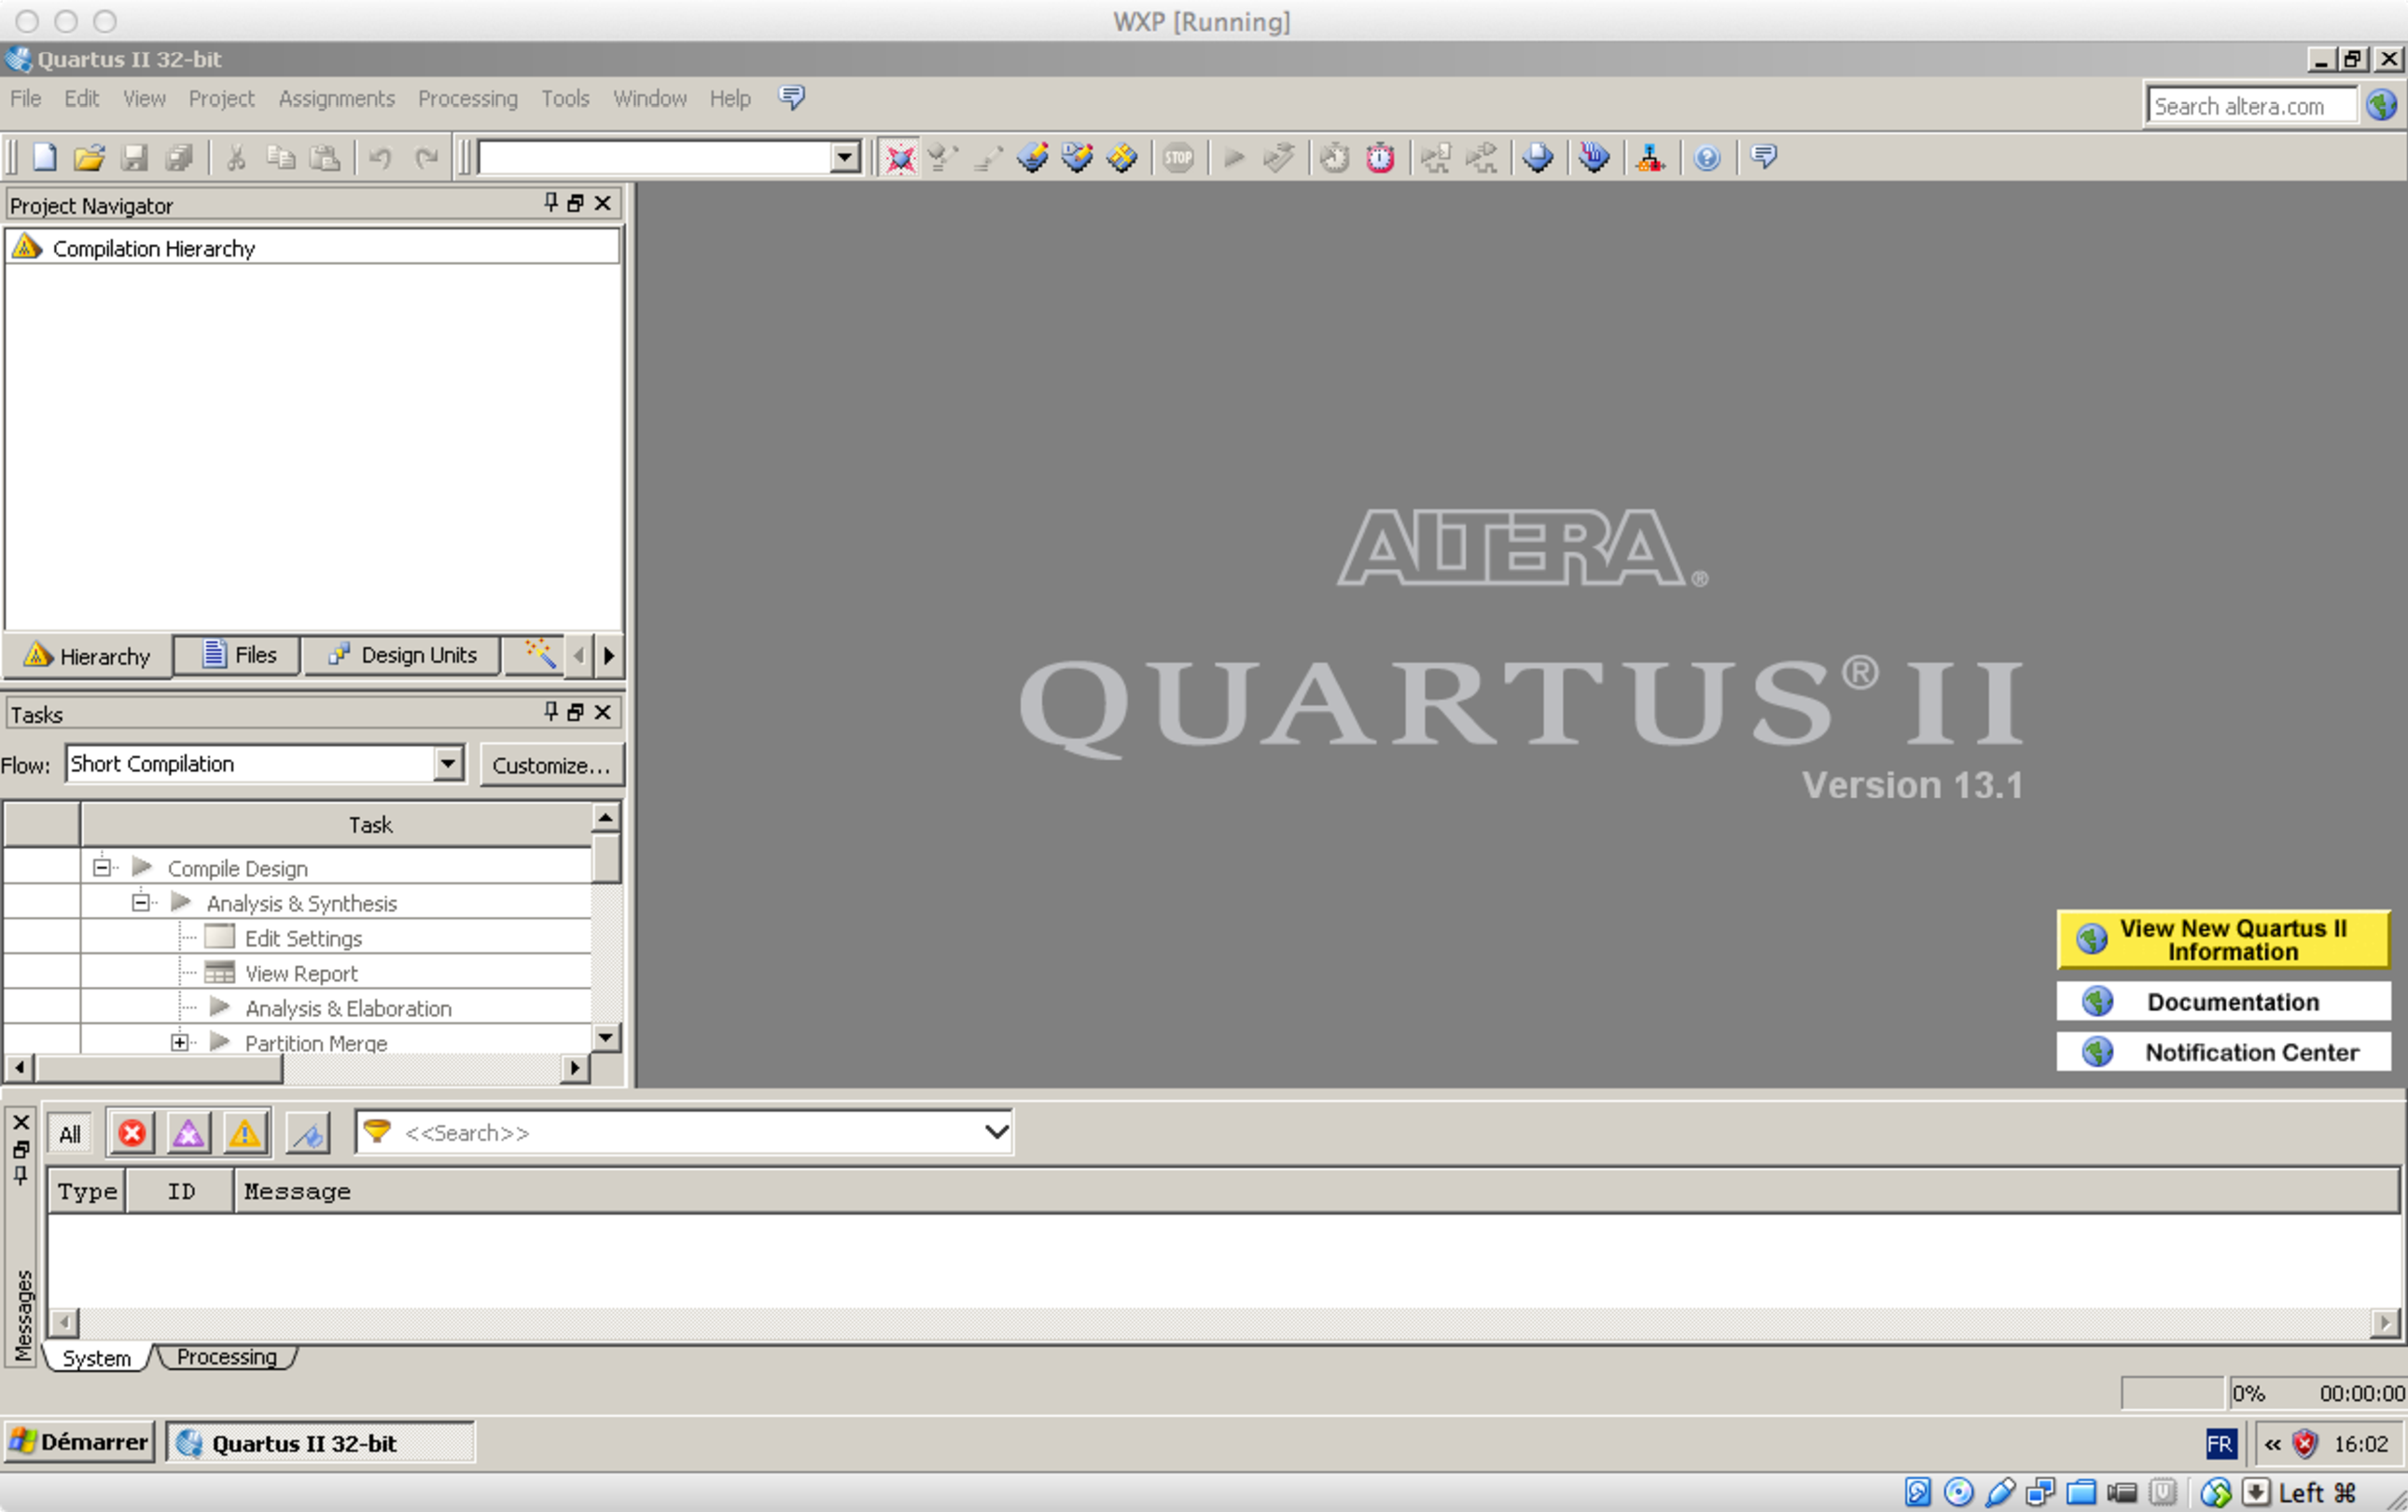
\includegraphics[angle=90,width=0.8\textwidth]{./figs/simple-quartus-1.pdf}
  \caption{The Quartus II environment, just after launching}
  \label{fig:simple-quartus-1}
\end{figure}

\begin{figure}[htbp]
  \centering
 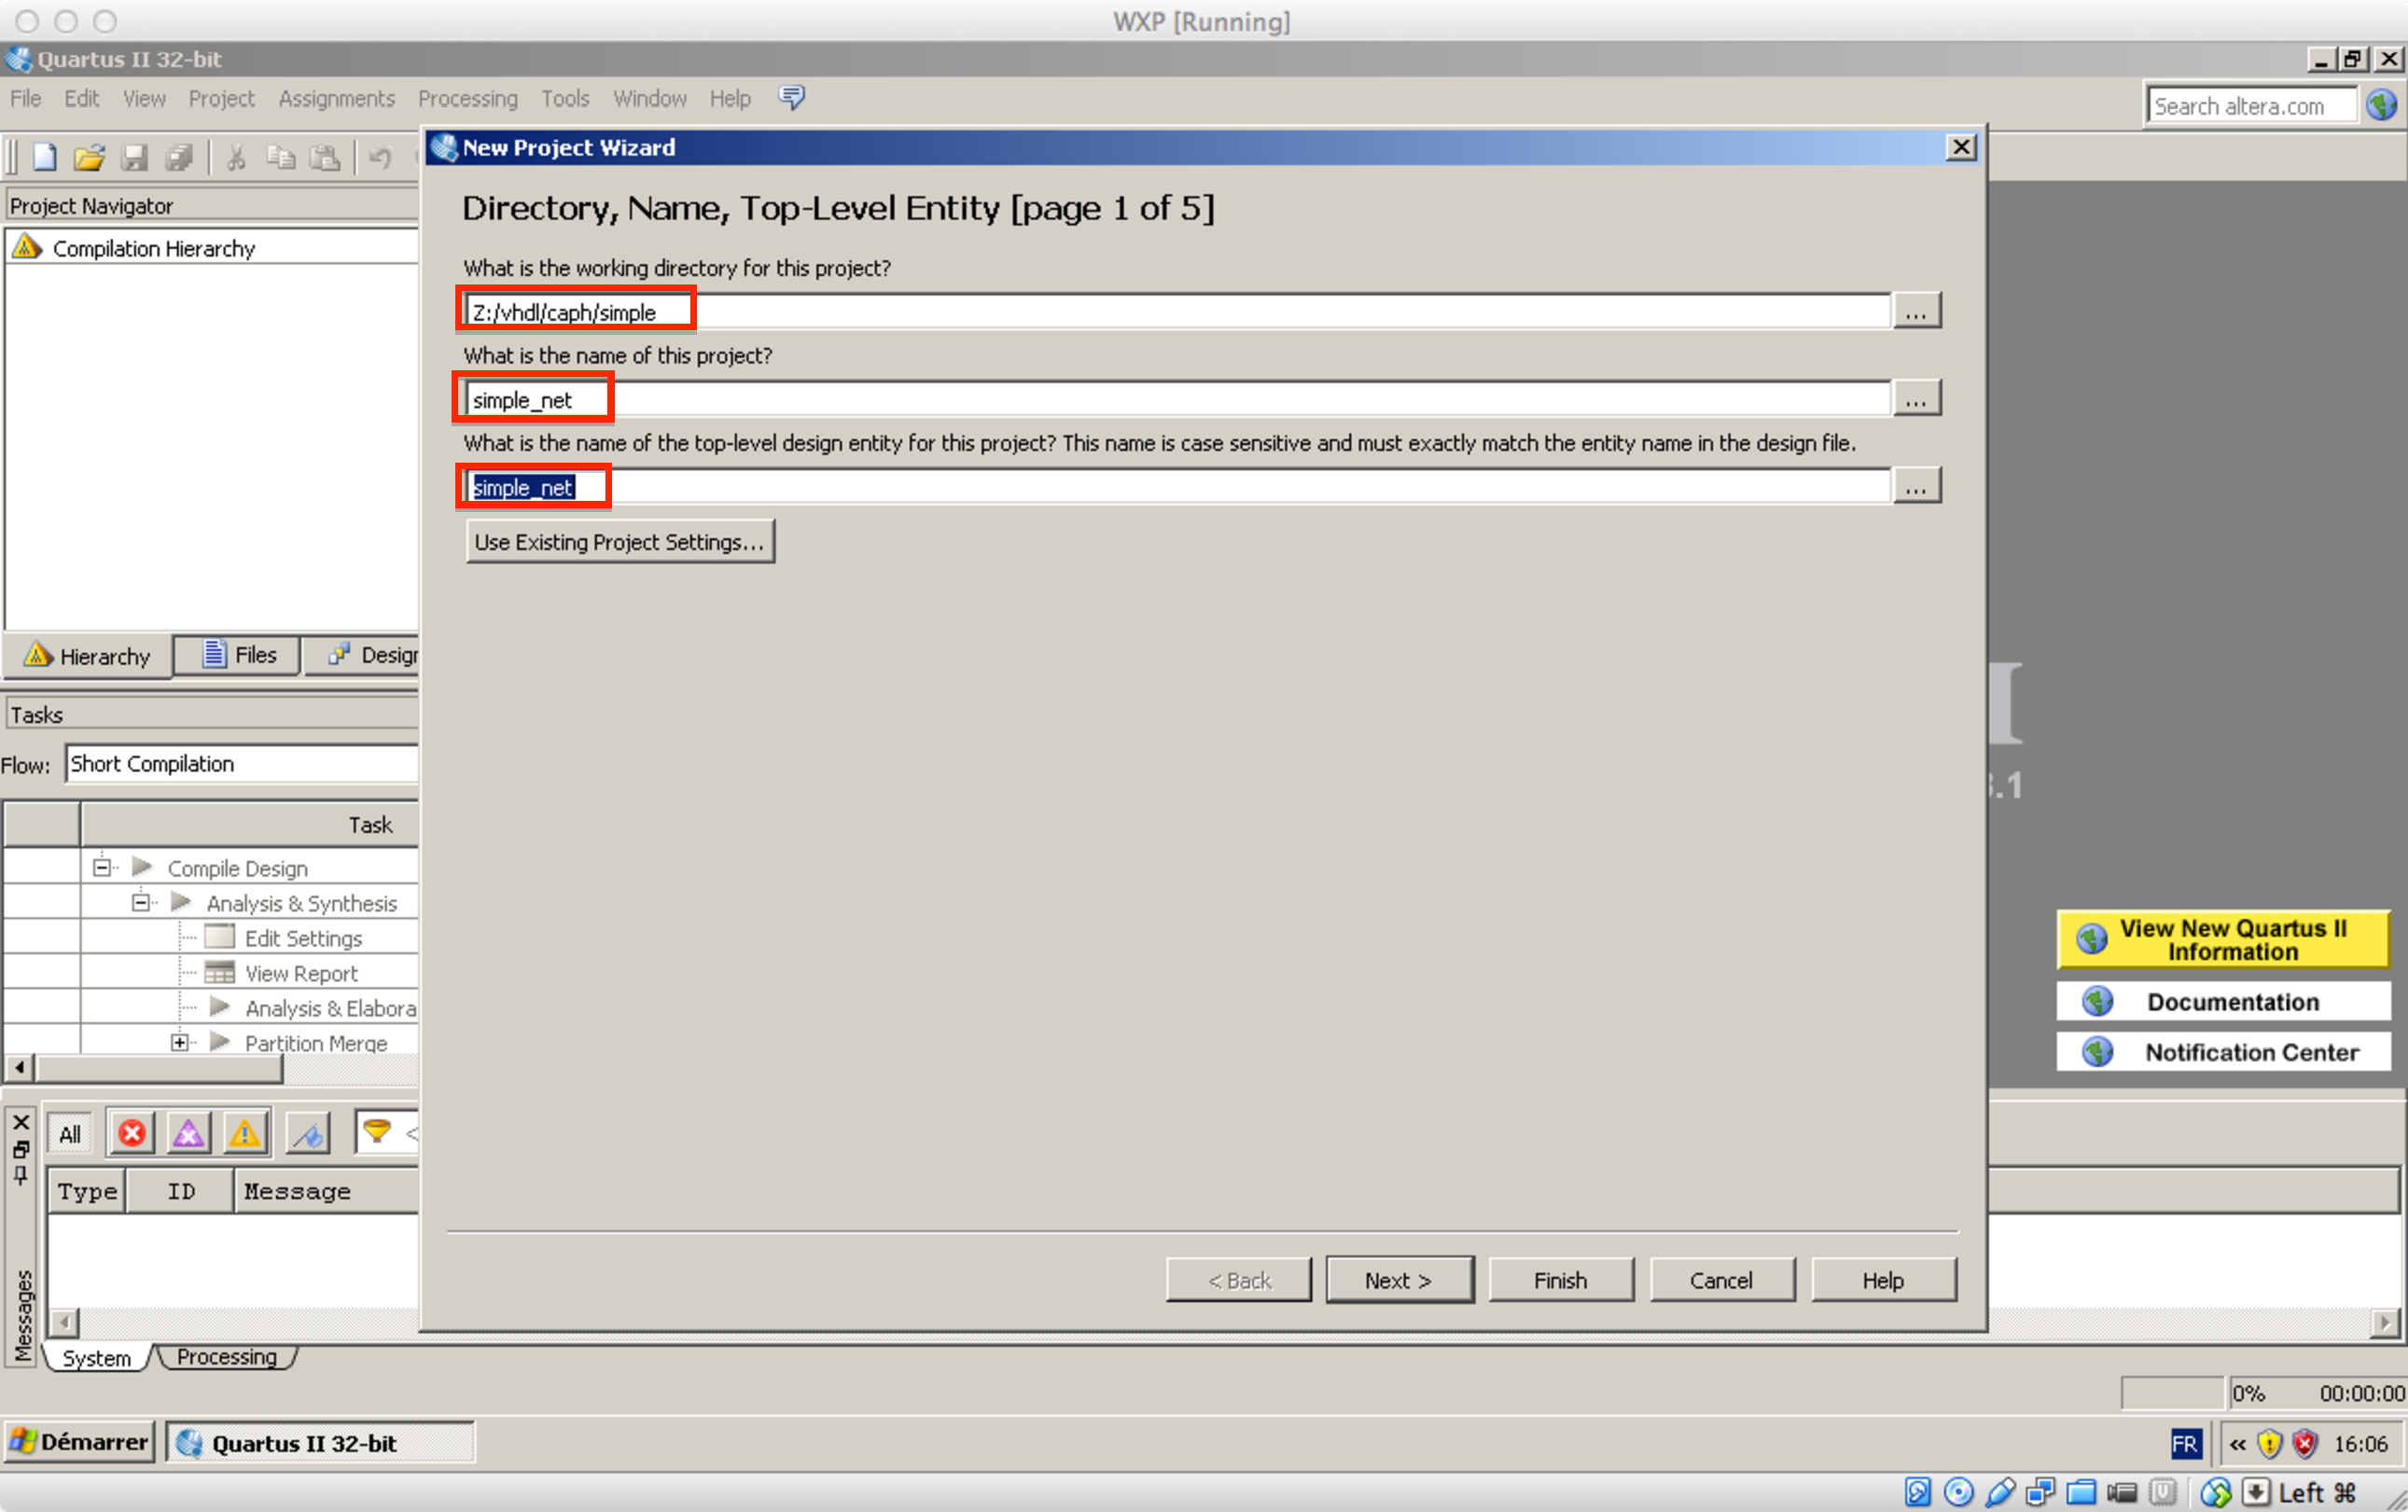
\includegraphics[angle=90,width=0.8\textwidth]{./figs/simple-quartus-2.pdf}
  \caption{Setting the projet - directory and top entity selection}
  \label{fig:simple-quartus-2}
\end{figure}

\begin{figure}[htbp]
  \centering
 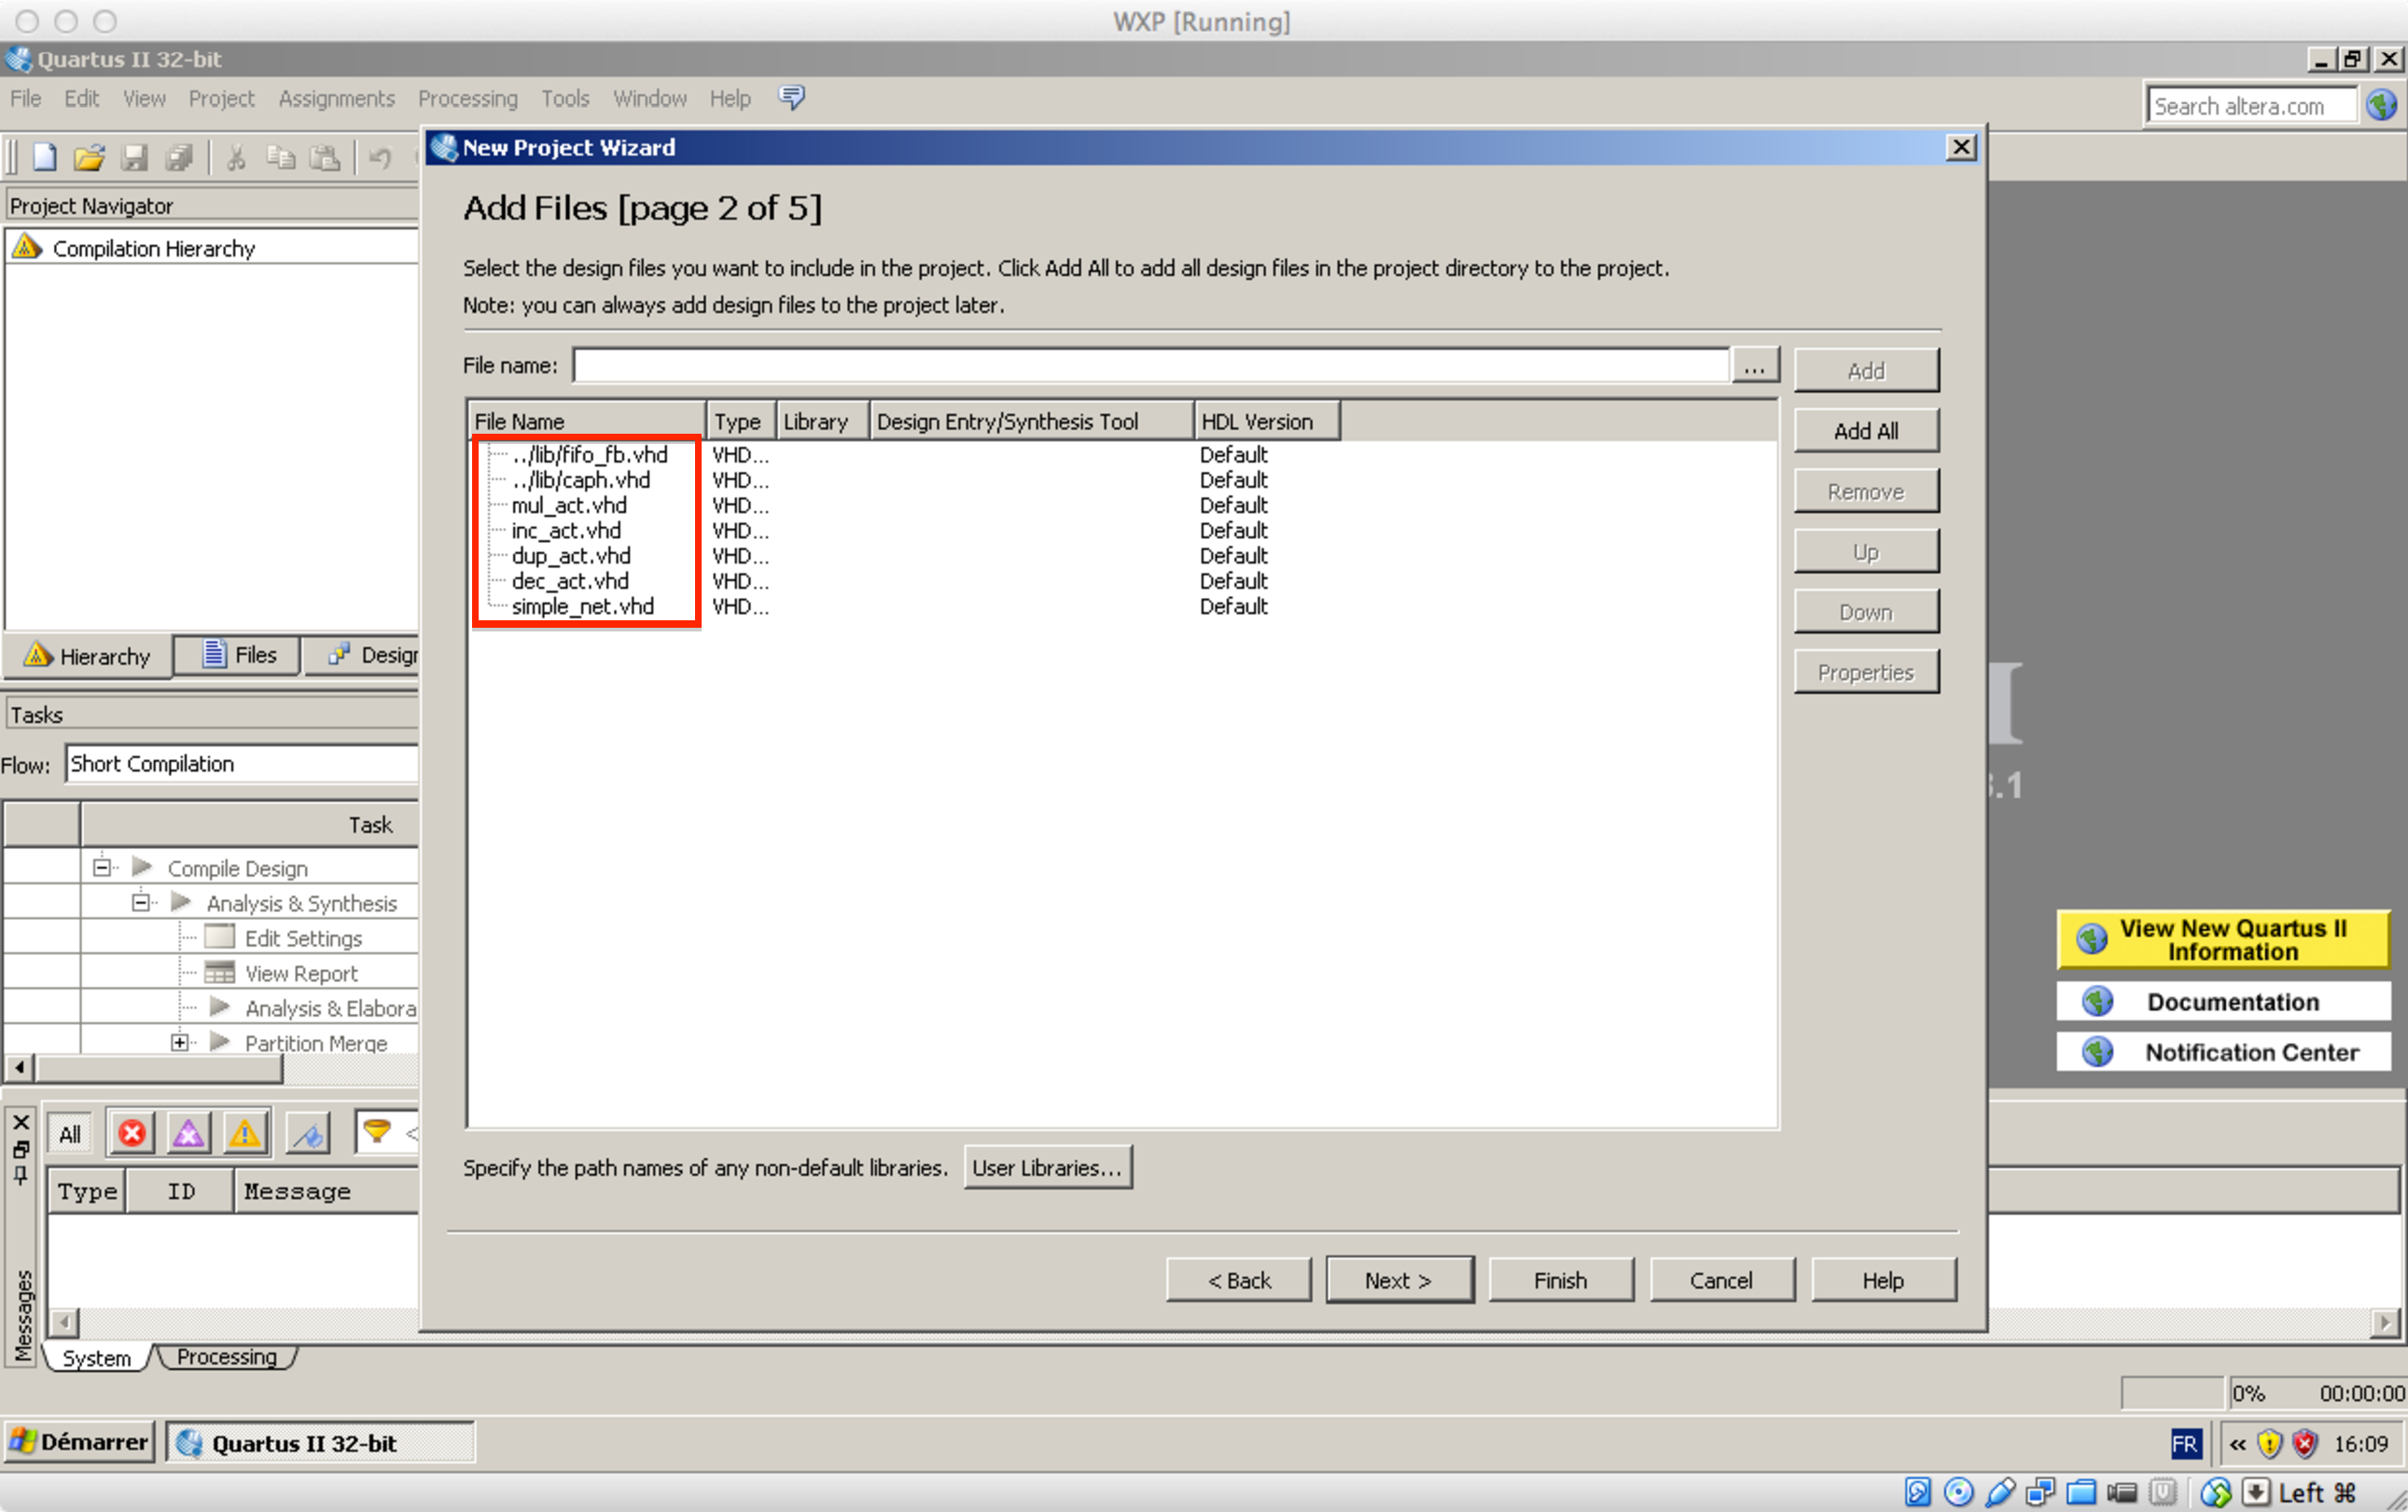
\includegraphics[angle=90,width=0.8\textwidth]{./figs/simple-quartus-3.pdf}
  \caption{Setting the source files of the project}
  \label{fig:simple-quartus-3}
\end{figure}

\begin{figure}[htbp]
  \centering
 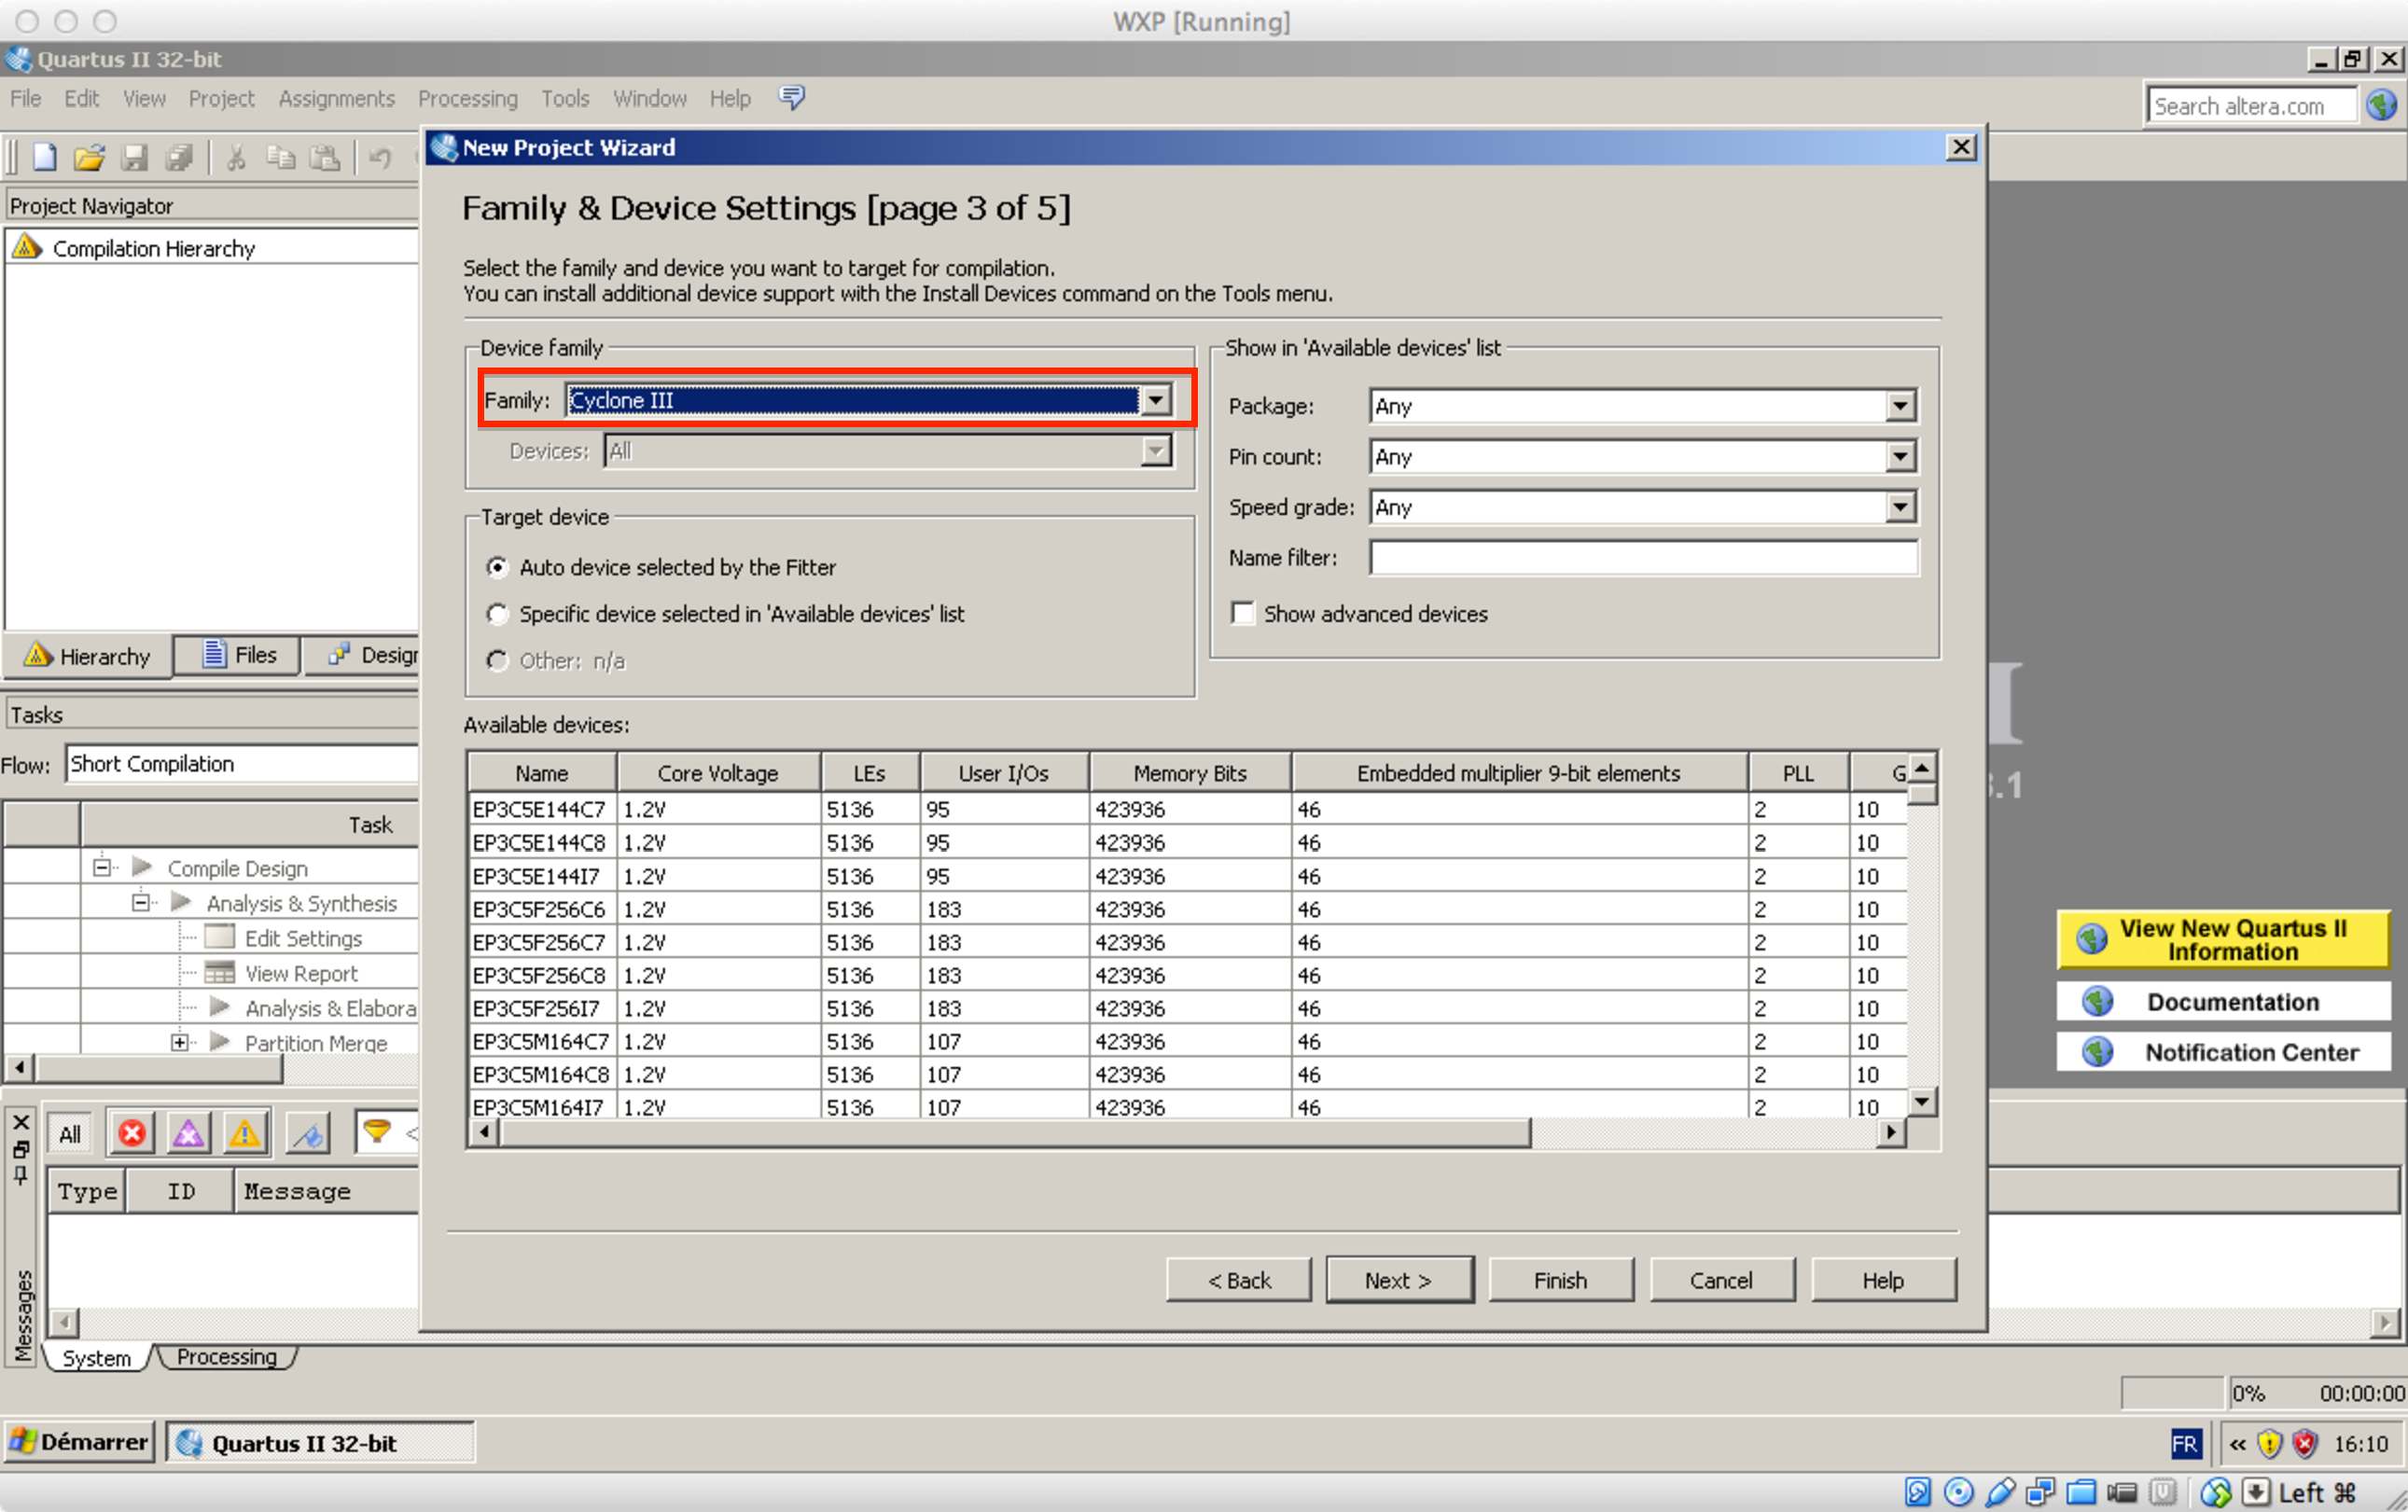
\includegraphics[angle=90,width=0.8\textwidth]{./figs/simple-quartus-4.pdf}
  \caption{Setting the target device}
  \label{fig:simple-quartus-4}
\end{figure}

\begin{figure}[htbp]
  \centering
 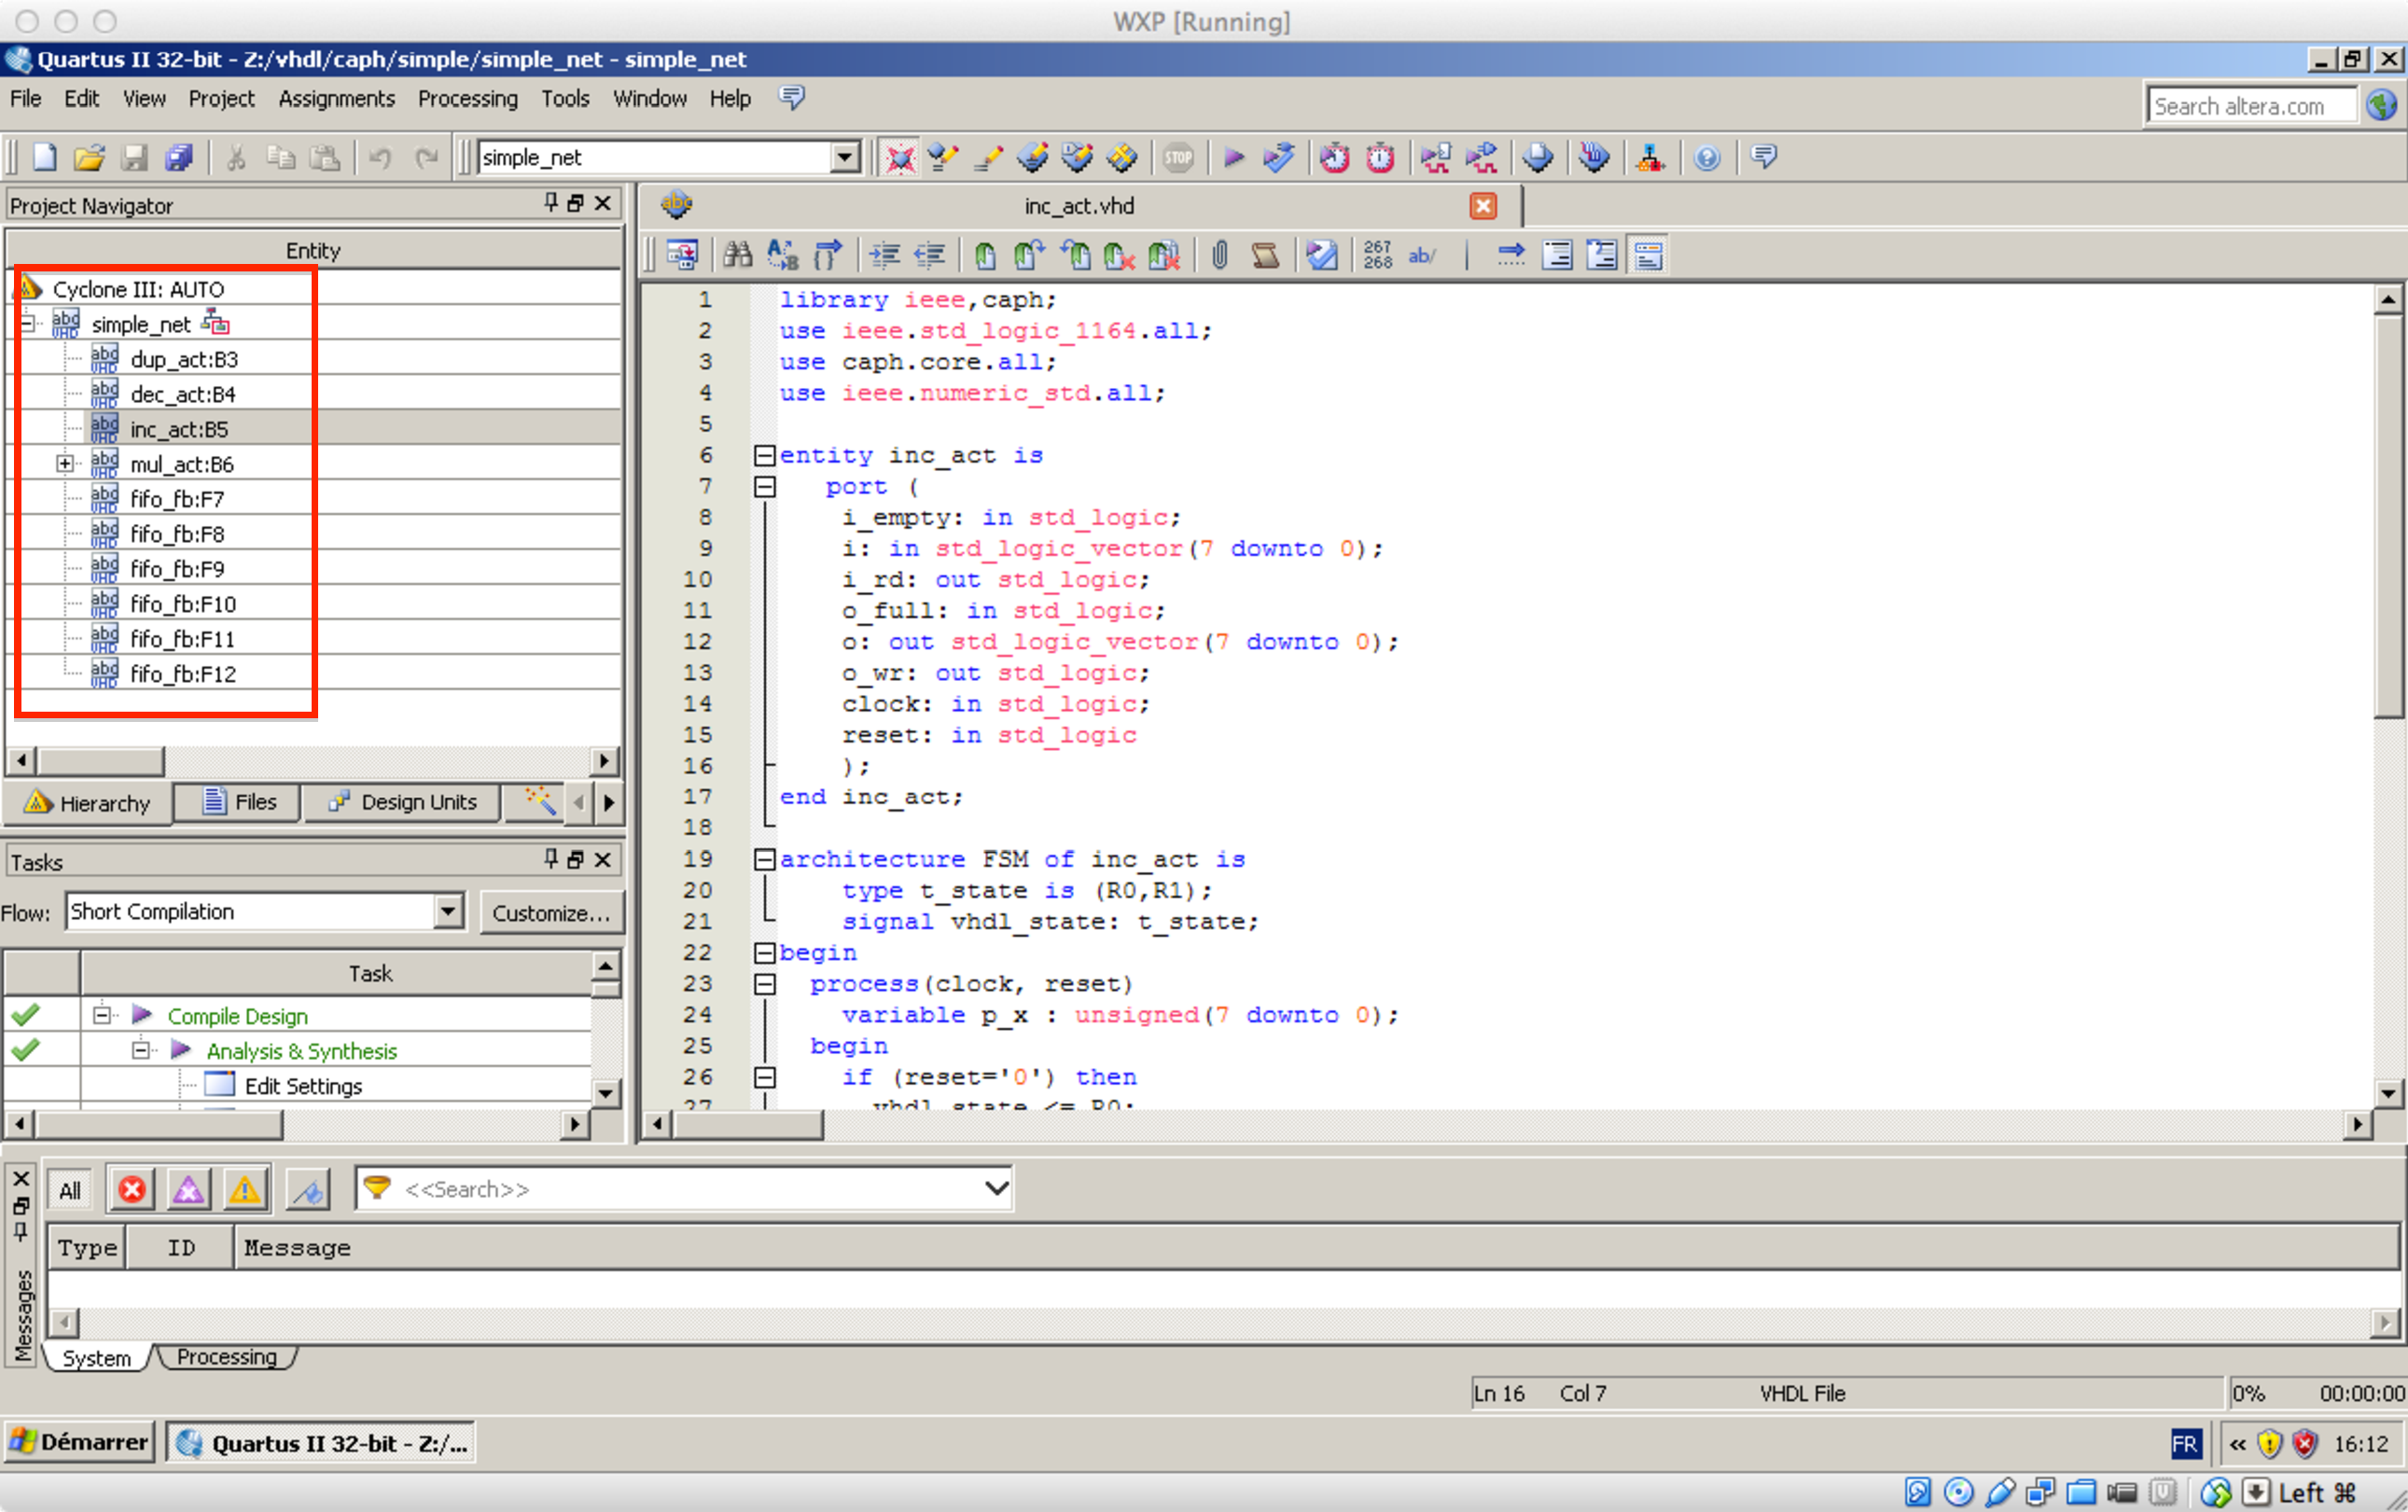
\includegraphics[angle=90,width=0.8\textwidth]{./figs/simple-quartus-5.pdf}
  \caption{Displaying design hierarchy and source files}
  \label{fig:simple-quartus-5}
\end{figure}

\begin{figure}[htbp]
  \centering
 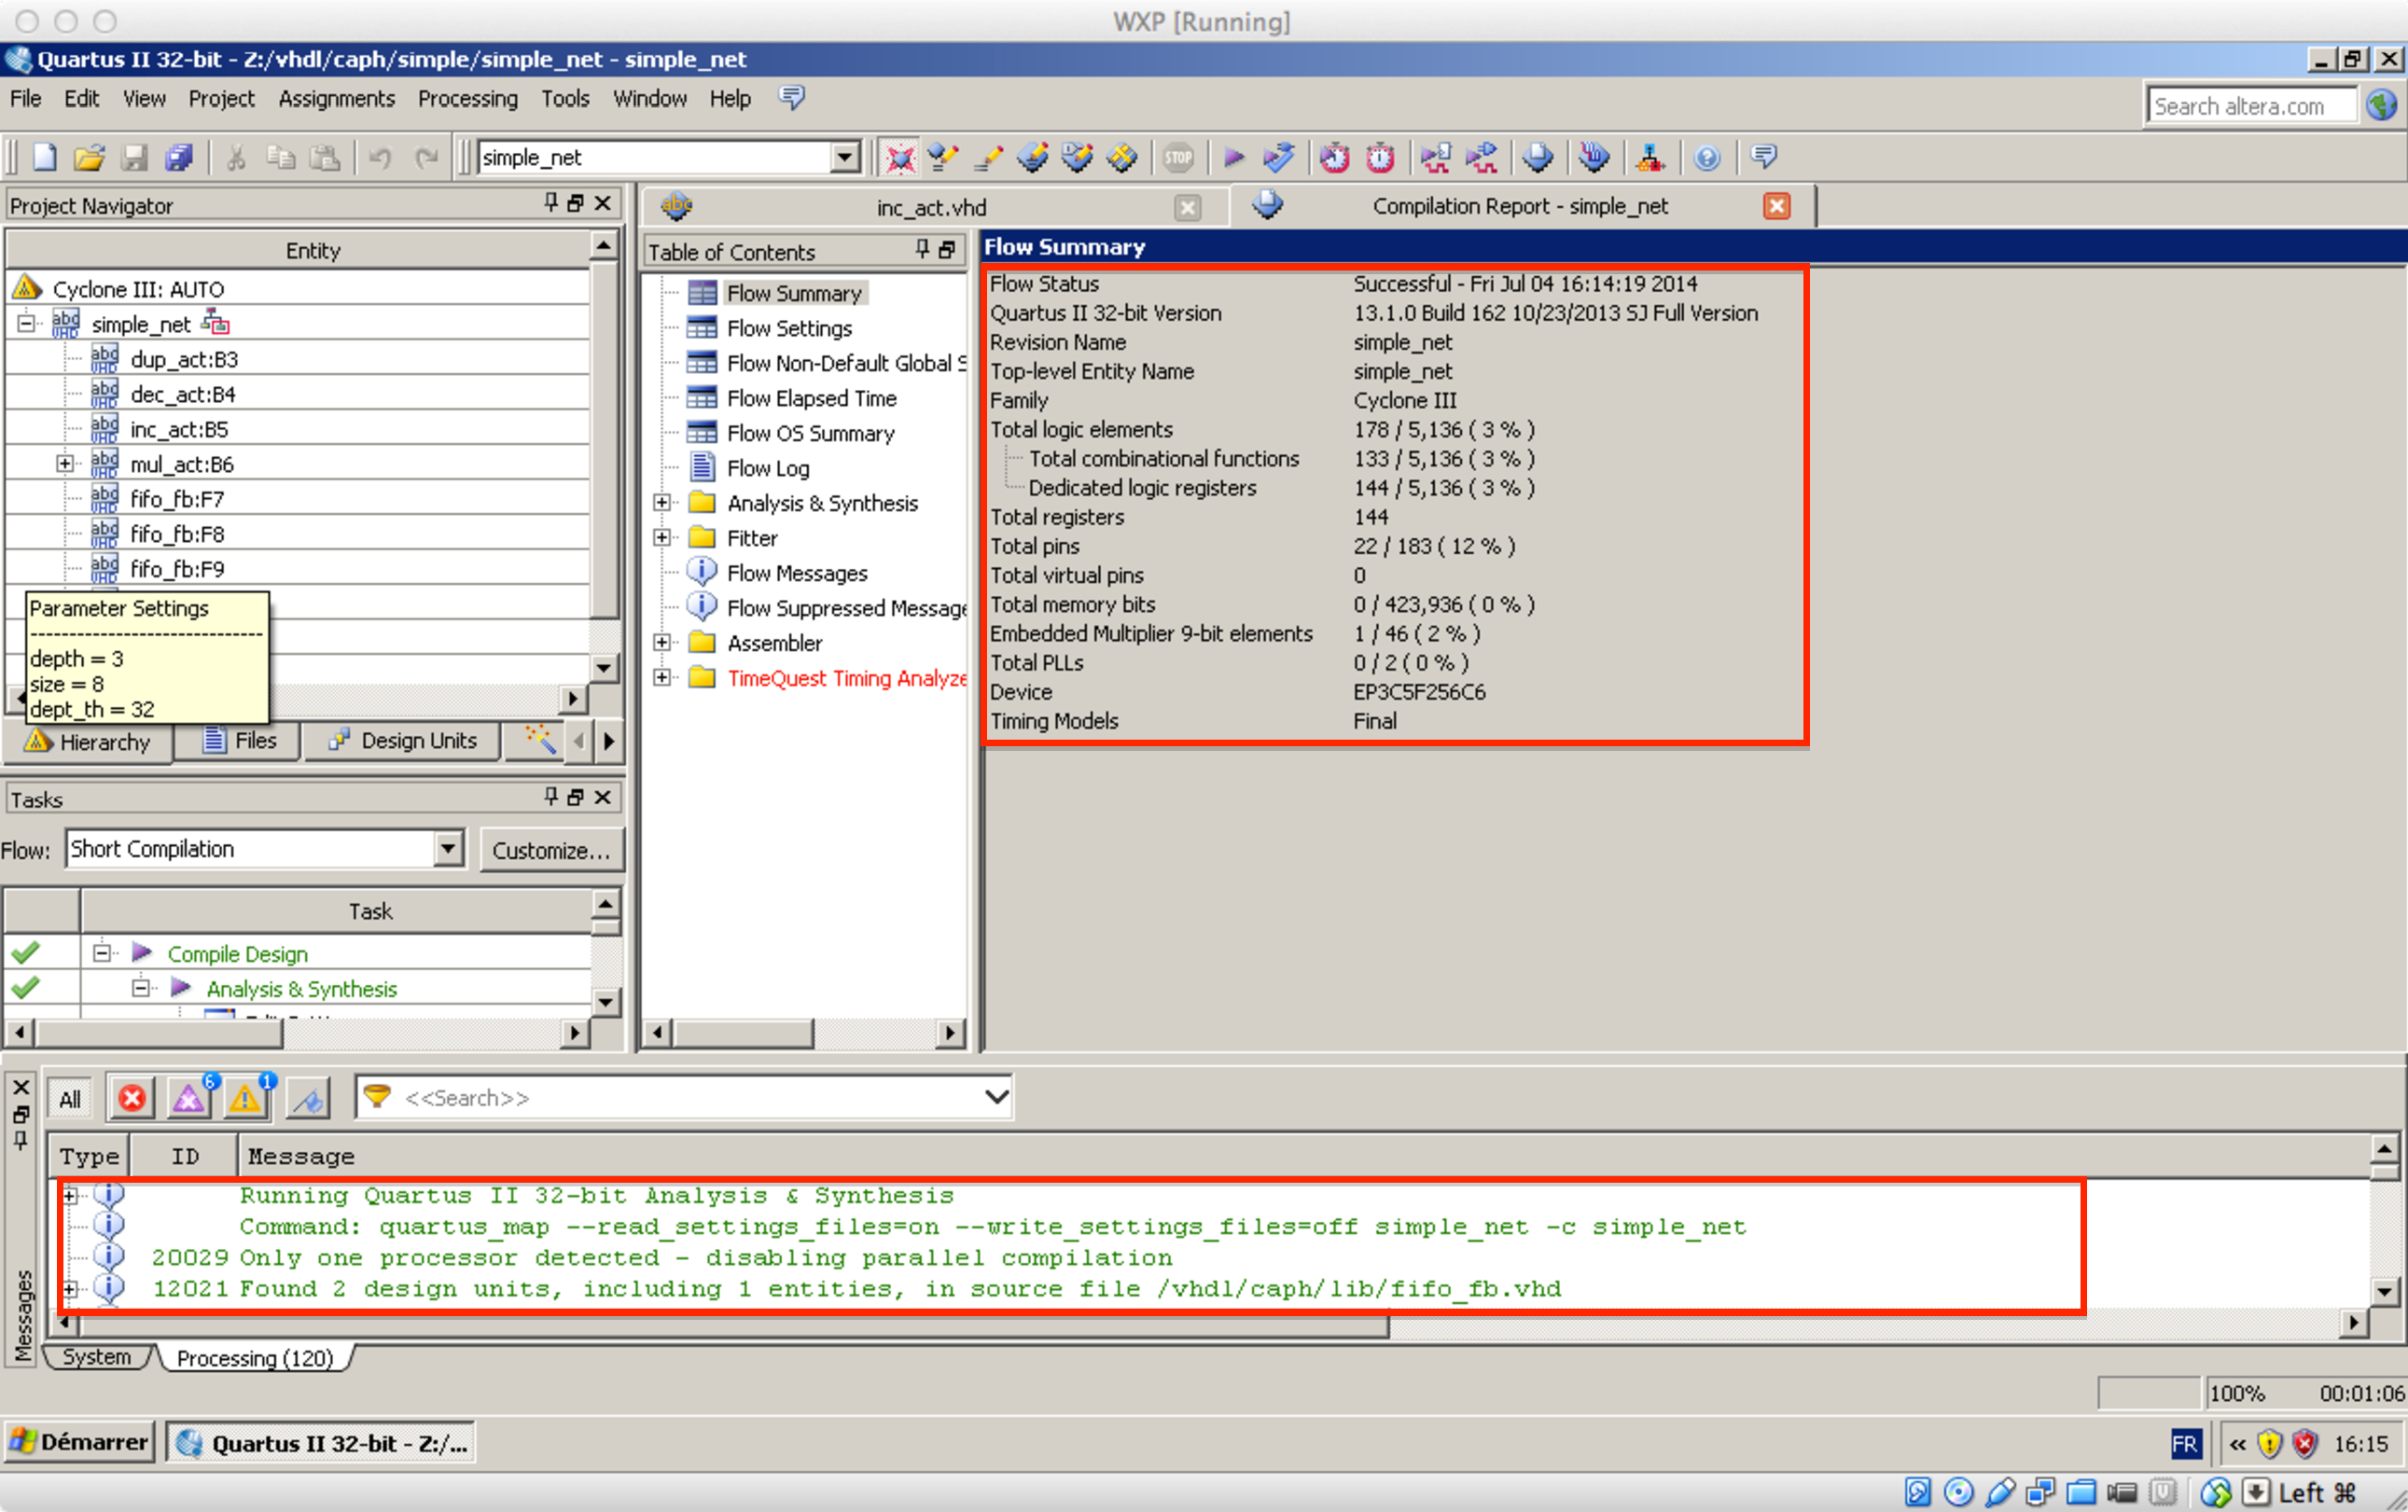
\includegraphics[angle=90,width=0.8\textwidth]{./figs/simple-quartus-6.pdf}
  \caption{Synthesis results}
  \label{fig:simple-quartus-6}
\end{figure}

\begin{figure}[htbp]
  \centering
 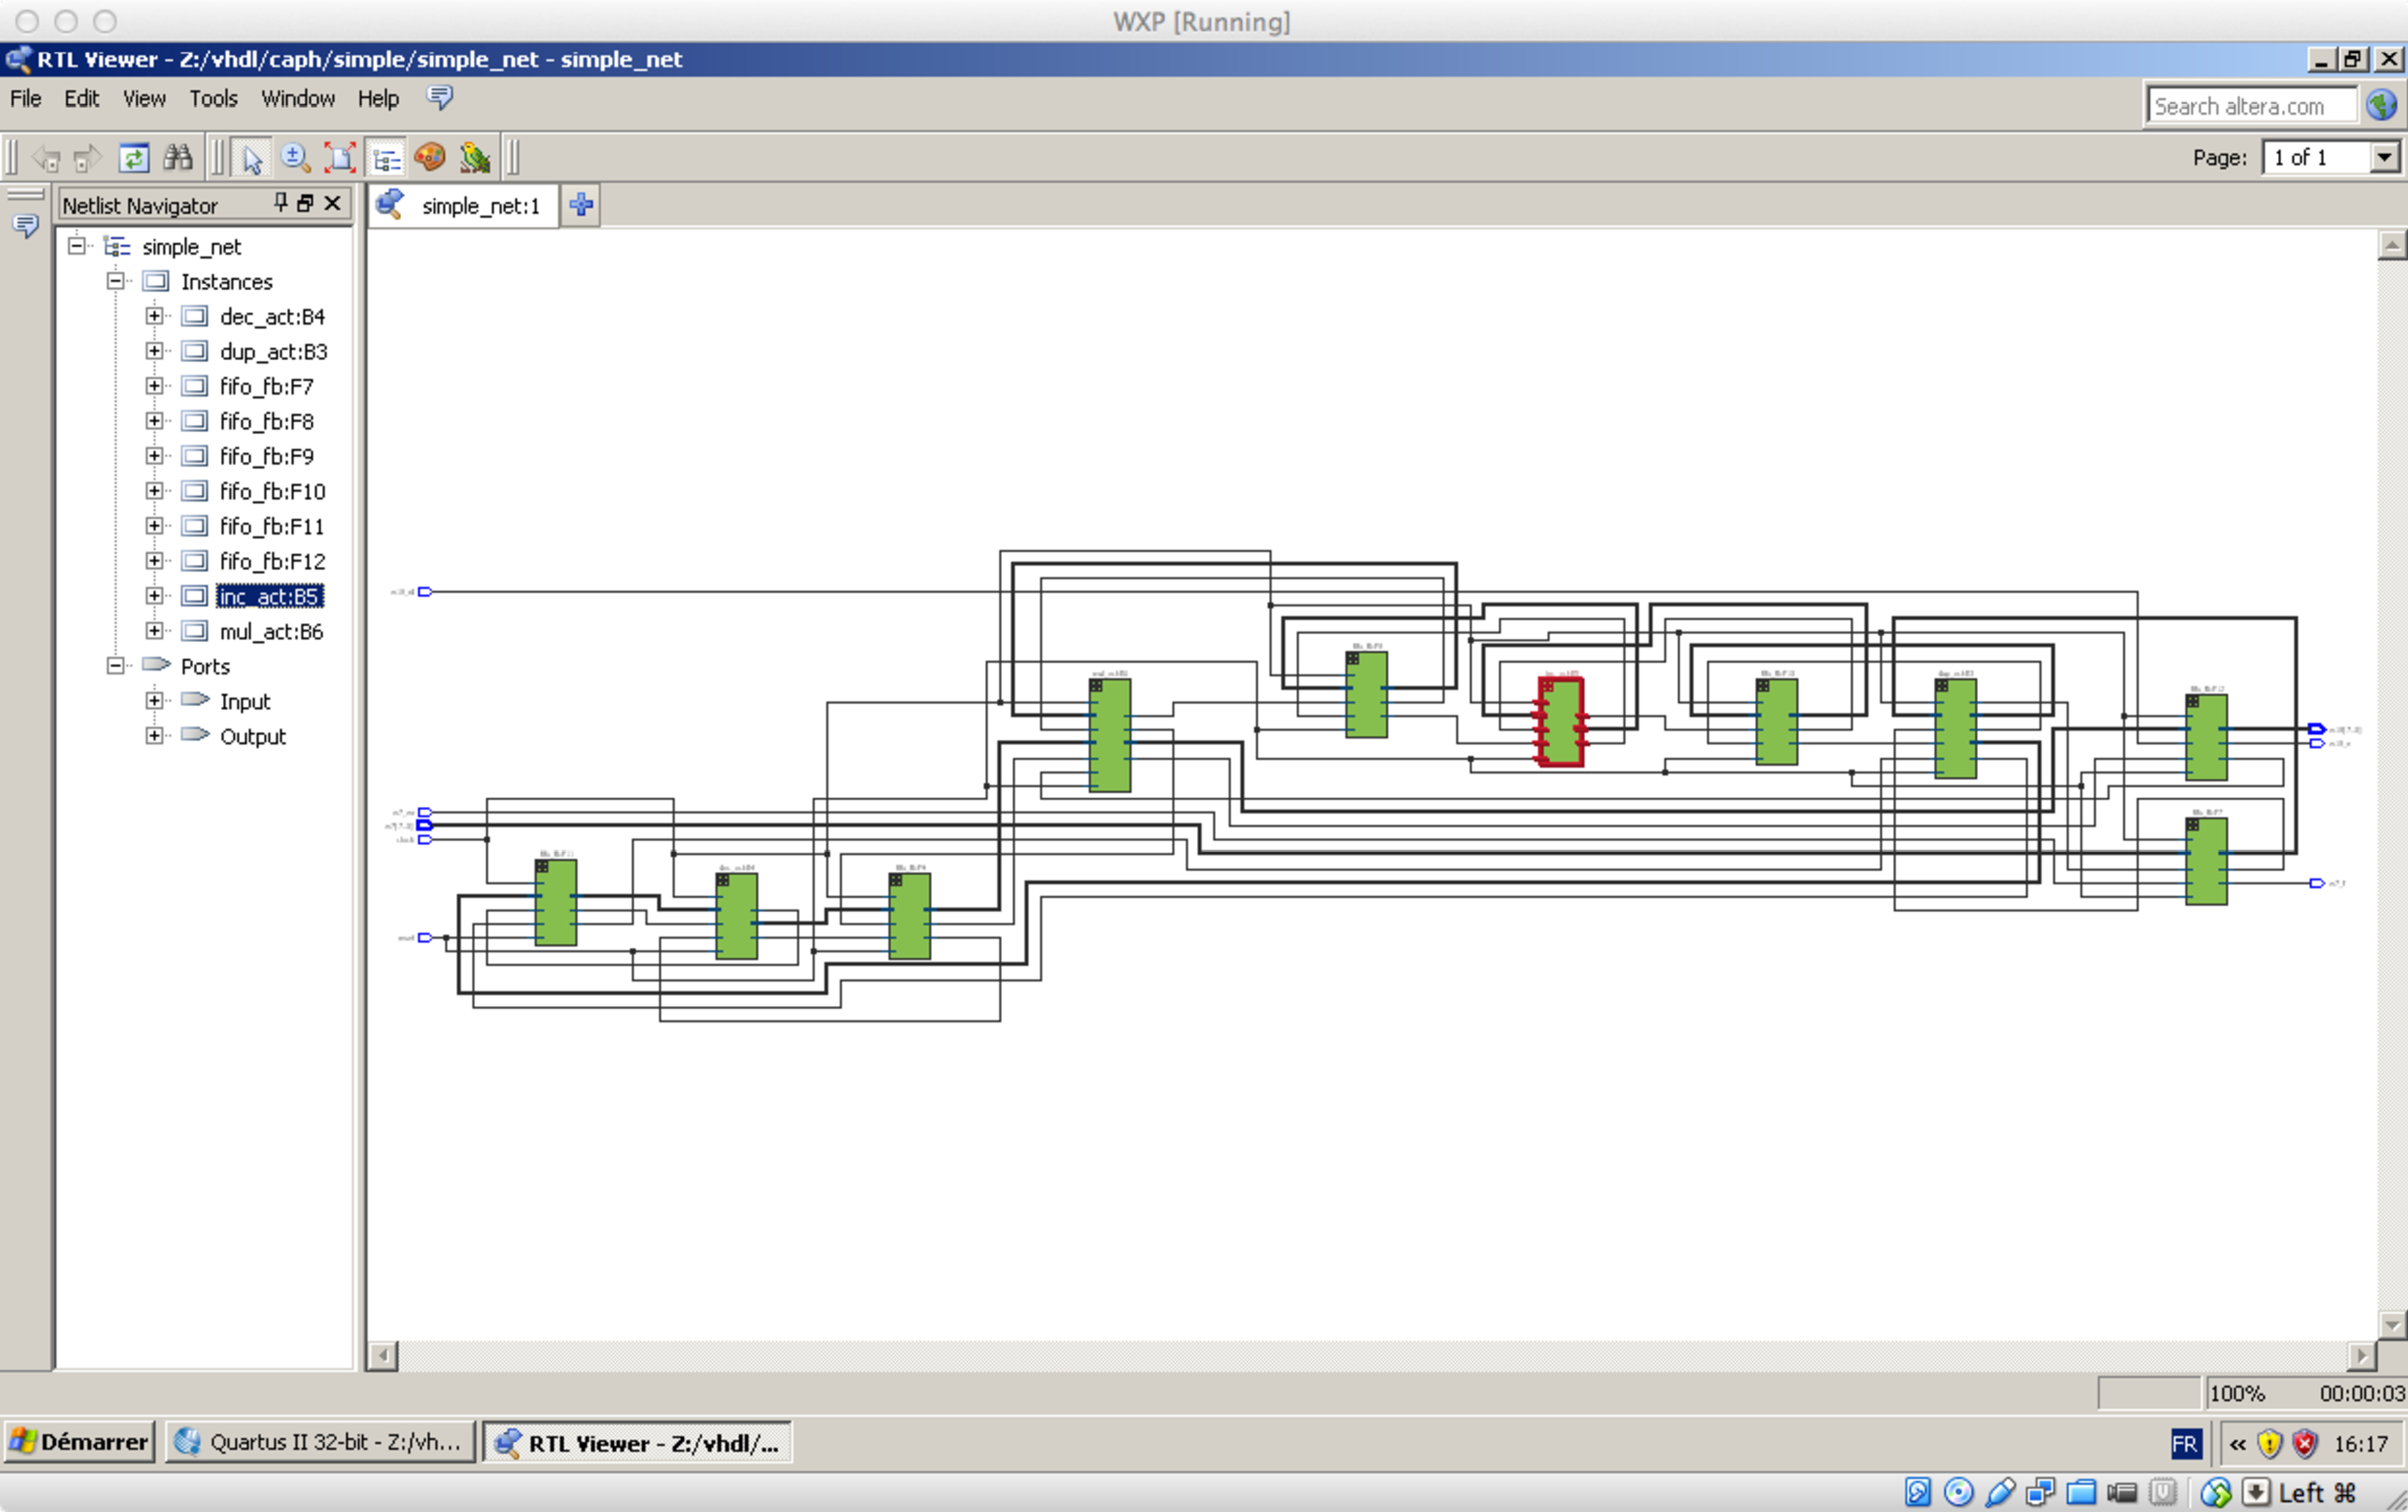
\includegraphics[angle=90,width=0.8\textwidth]{./figs/simple-quartus-7.pdf}
  \caption{Post-synthesis, RT-level view}
  \label{fig:simple-quartus-7}
\end{figure}

%%% Local Variables: 
%%% mode: latex
%%% TeX-master: "caph-primer"
%%% End: 

%%%%%%%%%%%%%%%%%%%%%%%%%%%%%%%%%%%%%%%%%%%%%%%%%%%%%%%%%%%%%%%%%%%%%%%%%%%%%%%%%%%%%%%%%
%%                                                                                     %%
%%                This file is part of the CAPH Compiler distribution                  %%
%%                            http:%/caph.univ-bpclermont.fr                           %%
%%                                                                                     %%
%%                                  Jocelyn SEROT                                      %%
%%                         Jocelyn.Serot@univ-bpclermont.fr                            %%
%%                                                                                     %%
%%         Copyright 2011-2018 Jocelyn SEROT.  All rights reserved.                    %%
%%  This file is distributed under the terms of the GNU Library General Public License %%
%%      with the special exception on linking described in file ..%LICENSE.            %%
%%                                                                                     %%
%%%%%%%%%%%%%%%%%%%%%%%%%%%%%%%%%%%%%%%%%%%%%%%%%%%%%%%%%%%%%%%%%%%%%%%%%%%%%%%%%%%%%%%%%

\chapter{Dealing with images}
\label{cha:cl-images}

This chapter describes the implementation, simulation and synthesis, using the command-line
interface, of the application based upon the concepts introduced in Chapter~\ref{cha:lang-images}. 

\medskip The code of this application, using the \texttt{inv} actor introduced in
Chapter~\ref{cha:lang-images}, is given in Listing~\ref{lst:invimg-full}. There's only \verb|net|
declaration, instantiating the \verb|inv| actor. The first line (\verb|#include "dc.cph"| is
mandatory for making use of the \verb|dc| type. The input image is to be read in file
\verb|lena128.pgm| and the result to be written in file \verb|result.pgm|\footnote{The PGM (Portable
  Graymap Format) is a portable format for representing gray level images introduced in the NetPBM
  projet~\cite{PGM}. \caph use the P2 (ASCII) sub-format.}.

\begin{lstlisting}[style=CaphStyle,caption={Complete CAPH source code for 
    an application computing negative images},label={lst:invimg-full}]
#include "dc.cph"

actor inv ()
  in (i:unsigned<8> dc)
  out (o:unsigned<8> dc)
rules
| i:'< -> o:'<
| i:'> -> o:'>
| i:'x -> o:'255-x
;

stream inp:unsigned<8> dc from "lena128.pgm";
stream outp:unsigned<8> dc to "result.pgm";

net outp = inv inp;\end{lstlisting}

\medskip
This program can be found in the \verb|examples/primer/invimg| directory in the CAPH distribution.

The corresponding project file (also to be found in the examples directory) is shown in
Listing~\ref{lst:invimg-proj}.  The option \verb|-abbrev-dc-ctors|, at lines 1 and 2, tells the
simulators (interpreter and SystemC-based, respectively) to read and write input and output files
using the abbreviated syntax for control tokens. 

\begin{lstlisting}[style=MakeStyle,caption={File
    \texttt{invimg.proj} for the \texttt{invimg} program of Listing~\ref{lst:invimg-full}},label={lst:invimg-proj}]
SIM_OPTS = -abbrev_dc_ctors
SC_OPTS = -sc_stop_time 1000000 -sc_abbrev_dc_ctors
GHDL_RUN_OPTS = --stop-time=400000ns
\end{lstlisting}

Let's build the top-level Makefile by typing

\begin{lstlisting}[style=BashInputStyle]
# caphmake
\end{lstlisting}

Then, the dataflow graphical representation of the program is easily obtained by invoking 

\begin{lstlisting}[style=BashInputStyle]
# make dot.show
\end{lstlisting}

The representation is shown in Fig.~\ref{fig:inv-dot}

\begin{figure}[htbp]
  \centering
 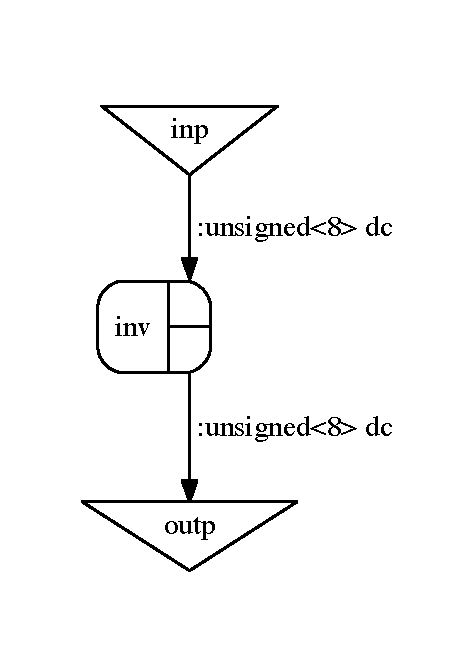
\includegraphics[width=0.3\textwidth]{./figs/inv-dot.pdf}
  \caption{The graphical representation of the program given in Listing.~\ref{lst:invimg-full}}
  \label{fig:inv-dot}
\end{figure}

\section{Simulation}
\label{sec:simulation-2}

The simulator cannot directly read and write images encoded with the PGM format. For this reason,
the CAPH distribution comes with a pair of utility programs, \verb|pgm2txt| and \verb|txt2pgm|, to
convert a PGM~\cite{PGM} file into a structured text file format and \emph{vice-versa} in which
pixels and start/end of line/frame are encoded using the \verb|dc| type introduced in
Chapter~\ref{sec:repr-imag}. A detailed description of these tools can be found in the reference
manual. They programs can called directly from the command line before and after launching the
simulation (to convert from and to the PGM format respectively), but this step can automatized
further by writing a dedicated auxilliary files called a \verb|.procs| file.  In our case, the
contents of this file (also to be found in the \verb|primer/invimg| directory) is reproduced in
Listing~\ref{lst:invimg-procs}.  The first line instructs the compiler to produce the file
\verb|lena128.txt| containing the input image in structured text format, ready for simulation, from
the input image file \verb|lena128.pgm|\footnote{The effect of the \texttt{-abbrev} option is to use
  the abbreviated format (\texttt{<}, \texttt{>}) for d(enoting control and data tokens. Without it,
  these tokens will be written as \texttt{SoS}, \texttt{EoS} and \texttt{Data} respectively.}.  The
second line instructs the compiler to produce the file \verb|result.pgm| containing the result image
in PGM format\footnote{As for \texttt{pgm2txt}, the \texttt{-abbrev} option indicates that the input
  text file uses the abbreviated format for tokens. The numerical argument (255, here) gives the
  maximum value to be written in the PGM file header.}.

\begin{lstlisting}[style=MakeStyle,caption={File
    \texttt{invimg.procs} for the \texttt{invimg} program of
    Listing~\ref{lst:invimg-full}},label={lst:invimg-procs}]
PRE_PROC = pgm2txt -abbrev lena128.pgm lena128.txt
POST_PROC = txt2pgm -abbrev 255 result.txt result.pgm
\end{lstlisting}

\medskip
Simulation is then performed simply by invoking

\begin{lstlisting}[style=BashInputStyle]
# make sim.makefile
# make sim
\end{lstlisting}

This yields the following output 

\begin{lstlisting}[style=BashOutputStyle]
make -f Makefile.sim run CAPH=/usr/local/caph
/usr/local/caph/bin/pgm2txt -abbrev lena128.pgm lena128.txt
/usr/local/caph/bin/caphc -sim -I /usr/local/caph/lib/caph -I /usr/local/caph/lib/caph -abbrev_dc_ctors main.cph
-------------------------------------------------------------------------------------------------
This is the Caph compiler, version 2.8.3
(C) 2011-2017 J. Serot (Jocelyn.Serot@univ-bpclermont.fr)
For more information, see : http://caph.univ-bpclermont.fr
-------------------------------------------------------------------------------------------------
Wrote file ./result.txt
\end{lstlisting}

Viewing the result image is obtained by typing

\begin{lstlisting}[style=BashInputStyle]
# make sim.show
\end{lstlisting}

This invokes the \verb|txt2pgm| utility and launch the PGM image viewing program which has been
specified when installing \caph. In our case, the results are show below and in
Fig.~\ref{fig:inv-result}-b.

\begin{lstlisting}[style=BashOutputStyle]
make -f Makefile.sim show CAPH=/usr/local/caph
/usr/local/caph/bin/txt2pgm -abbrev 255 result.txt result.pgm
open -a Toyviewer result.pgm
\end{lstlisting}

\begin{figure}[htbp]
  \centering
  \begin{tabular}[c]{cc}
 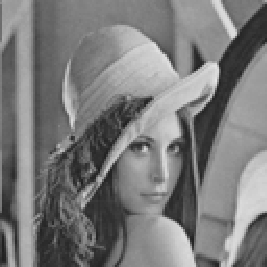
\includegraphics[width=0.3\textwidth]{./figs/lena128.pdf} &
 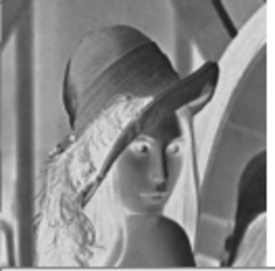
\includegraphics[width=0.3\textwidth]{./figs/inv-result.pdf} \\
 a & b
  \end{tabular}
  \caption{Input and output images after simulation for the program given in Listing.~\ref{lst:invimg-full}}
  \label{fig:inv-result}
\end{figure}

\section{Simulation using the SystemC backend}
\label{sec:simul-using-sysc-2}

As in the previous chapter, this is done by simply typing 

\begin{lstlisting}[style=BashInputStyle]
# make systemc.makefile
# make systemc.run
\end{lstlisting}

Executing this command yields the following output 

\begin{lstlisting}[style=BashOutputStyle]
make -f Makefile.systemc run CAPH=/usr/local/caph
/usr/local/caph/bin/caphc -I /usr/local/caph/lib/caph -systemc -I /usr/local/caph/lib/caph -sc_stop_time 1000000 -sc_abbrev_dc_ctors  main.cph
...
Wrote file ./invimg_expanded.dot
Wrote file ./invimg_net.cpp
Wrote file ./invimg_globals.h
Wrote file ./invimg_globals.cpp
Wrote file ./inv_act.h
Wrote file ./inv_act.cpp
(cd .; g++ -std=c++11 -I. -I/usr/local/caph/lib/systemc ... -c `basename inv_act.cpp`)
(cd .; g++ -std=c++11 -I. -I/usr/local/caph/lib/systemc ... -c `basename invimg_globals.cpp`)
(cd .; g++ -std=c++11 -I. -I/usr/local/caph/lib/systemc ... -c `basename invimg_net.cpp`)
(cd .; g++ -L/usr/local/systemc-2.3.1/lib-macosx64 inv_act.o invimg_globals.o invimg_net.o
   -o invimg_sc -lsystemc  2>&1 | c++filt)
./invimg_sc
        SystemC 2.3.1-Accellera --- Aug  9 2015 15:42:56
        Copyright (c) 1996-2014 by all Contributors,
        ALL RIGHTS RESERVED
Simulation stopped at t=1 ms
\end{lstlisting}

Viewing the file \verb|result.txt| is then handled exactly like above, by invoking 

\begin{lstlisting}[style=BashInputStyle]
# make systemc.show
\end{lstlisting}

\section{Generating and  simulating VHDL code}
\label{sec:generating-vhdl-2}

The process, again, is similar. Simply type

\begin{lstlisting}[style=BashInputStyle]
# make vhdl.makefile
# make vhdl.run
\end{lstlisting}

Executing this command yields the following output 

\begin{lstlisting}[style=BashOutputStyle]
make -f Makefile.vhdl run CAPH=/usr/local/caph
/usr/local/caph/bin/caphc -I /usr/local/caph/lib/caph -vhdl -I /usr/local/caph/lib/caph main.cph
...
Wrote file ./invimg_expanded.dot
Reverting to default size for fifo F5
Reverting to default size for fifo F4
Wrote file ./invimg_net.vhd
Wrote file ./invimg_types.vhd
Wrote file ./inv_act.vhd
Wrote file ./invimg_tb.vhd
warning: VHDL annotation file fifo_caps.dat does not exist.
(cd .; ghdl -a -P/usr/local/caph/lib/vhdl `basename invimg_types.vhd`)
(cd .; ghdl -a -P/usr/local/caph/lib/vhdl `basename invimg_tb.vhd`)
(cd .; ghdl -a -P/usr/local/caph/lib/vhdl `basename inv_act.vhd`)
(cd .; ghdl -a -P/usr/local/caph/lib/vhdl `basename invimg_net.vhd`)
(cd .; ghdl -e -P/usr/local/caph/lib/vhdl invimg_tb)
/usr/local/caph/bin/pgm2bin 8 lena128.pgm lena128.bin
ghdl -r -P/usr/local/caph/lib/vhdl invimg_tb --stop-time=400000ns  
./invimg_tb:info: simulation stopped by --stop-time
\end{lstlisting}

Viewing the file \verb|result.txt| is then handled exactly like above, by invoking 

\begin{lstlisting}[style=BashInputStyle]
# make vhdl.show
\end{lstlisting}

The only difference here with the steps described in the previous section concerns the
generation of the input file(s) and the conversion of the output file(s) to/from the custom
\verb|bin| format used by the VHDL simulator. The utility programs to use are now \verb|pgm2bin| and
\verb|bin2pgm| respectively\footnote{These programs are also included in the CAPH
  distribution.}. The corresponding calls to these utility programs are automatically inserted in
the VHDL-specific Makefile generated by \verb|caphmake|.

%%% Local Variables: 
%%% mode: latex
%%% TeX-master: "caph-primer"
%%% End: 

%%%%%%%%%%%%%%%%%%%%%%%%%%%%%%%%%%%%%%%%%%%%%%%%%%%%%%%%%%%%%%%%%%%%%%%%%%%%%%%%%%%%%%%%%
%%                                                                                     %%
%%                This file is part of the CAPH Compiler distribution                  %%
%%                            http:%/caph.univ-bpclermont.fr                           %%
%%                                                                                     %%
%%                                  Jocelyn SEROT                                      %%
%%                         Jocelyn.Serot@univ-bpclermont.fr                            %%
%%                                                                                     %%
%%         Copyright 2011-2018 Jocelyn SEROT.  All rights reserved.                    %%
%%  This file is distributed under the terms of the GNU Library General Public License %%
%%      with the special exception on linking described in file ..%LICENSE.            %%
%%                                                                                     %%
%%%%%%%%%%%%%%%%%%%%%%%%%%%%%%%%%%%%%%%%%%%%%%%%%%%%%%%%%%%%%%%%%%%%%%%%%%%%%%%%%%%%%%%%%

\chapter{Image processing}
\label{cha:cl-ip}

This chapter describes the implementation, simulation and synthesis, using the command-line
interface, of the \emph{Sobel} application introduced in Chapter~\ref{cha:lang-ip}. 

The code of this application has been given in Listing.~\ref{lst:sobel-full}. The related project
can be found in the directory \verb|examples/primer/sobel| of the distribution.

\section{Simulation using the interpreter}
\label{sec:simulation-3}

The simulation process is completely similar to the one described in Chapter~\ref{cha:cl-images}.
The project description file is reproduced in Listing~\ref{lst:sobel-proj}.

\begin{lstlisting}[style=MakeStyle,caption={Project file for the program of in Listing.~\ref{lst:sobel-full}},label={lst:sobel-proj}]
DOT_OPTS = -D ifile=pcb.pgm -D threshold=80 -suppress_cast_warnings
SIM_OPTS = -D ifile=pcb.pgm -D threshold=80 -suppress_cast_warnings -abbrev_dc_ctors -warn_channels -dump_channel_stats
SC_OPTS = -D ifile=pcb.pgm -D threshold=80 -suppress_cast_warnings -sc_abbrev_dc_ctors -sc_stop_when_idle 1000 -sc_dump_fifo_stats
VHDL_OPTS = -D ifile=pcb.pgm -D threshold=80 -suppress_cast_warnings -vhdl_annot_file sobel_fifo_stats.dat
GHDL_RUN_OPTS = --stop-time=160000ns
\end{lstlisting}
%$

The \verb|-D| option is used is give values to the symbols named \verb|%ifile| and \verb|%threshold|
in the source code. 

The option \verb|-suppress_cast_warnings| is used to omit warning messages
which are emitted when compiling the \verb|fabs| function and which, in this context, can be safely
ignored.

The \verb|-warn_channels| option is set in order to detect channel overflows and the
\verb|-dump_channel_stats| is set in order to check channel usage after run. 

\medskip The \verb|.procs| file for this application, given in Listing~\ref{lst:sobel-procs}, is
similar to that given in the previous chapter. It simply tells how to convert from and to PGM format
for the input and output images.

\begin{lstlisting}[style=MakeStyle,caption={File
    \texttt{sobel.procs} for the \texttt{sobel} program of
    Listing~\ref{lst:sobel-full}},label={lst:sobel-procs}]
PRE_PROC = pgm2txt -abbrev pcb.pgm pcb.txt
POST_PROC = txt2pgm -abbrev 255 sim/result.txt sim/result.pgm
\end{lstlisting}

\medskip
Simulation is performed, as usual with the following sequence of commands :

\begin{lstlisting}[style=BashInputStyle]
# caphmake
# make sim.makefile
# make sim.run
\end{lstlisting}

It produces the following result\footnote{Warning, this can take a few seconds} :

\begin{lstlisting}[style=BashOutputStyle]
make -f Makefile.sim run CAPH=/usr/local/caph
/usr/local/caph/bin/pgm2txt -abbrev pcb.pgm pcb.txt
/usr/local/caph/bin/caphc -sim -I /usr/local/caph/lib/caph -I /usr/local/caph/lib/caph -D ifile=pcb.pgm -D threshold=80 -suppress_cast_warnings -abbrev_dc_ctors -warn_channels -dump_channel_stats main.cph
...
Wrote file ./result.txt
W3: occ=0/256 max=2
W2: occ=140/256 max=140
W1: occ=140/256 max=140
W6: occ=0/256 max=2
W5: occ=140/256 max=140
W4: occ=140/256 max=140
W8: occ=0/256 max=2
W7: occ=0/256 max=2
W9: occ=0/256 max=2
W10: occ=0/256 max=2
\end{lstlisting}

Displaying the output image (Fig.~\ref{fig:sobel-result}-b) is obtained by invoking

\begin{lstlisting}[style=BashInputStyle]
# make sim.show
\end{lstlisting}

\medskip
The maximum occupation reported for channels \verb|W1|, \verb|W2|, \verb|W5| and \verb|W4| is worth
to be noted. The corresponding channels are used by the \verb|conv233| actor to memorize the two
previous lines when computing the convolution\footnote{These channels are those ``looping around''
  the \texttt{conv233} actors in Fig.~\ref{fig:sobel-full}.}. The maximum occupation value
corresponds here to the width in pixels of the input image (140). No overflow occured because the
default depth of channels in simulation is 256. Should we have used a larger image (ex: $512 \times
512$), it would have been necessary to adjust this depth with the \verb|-chan_cap| option.

\begin{figure}[htbp]
  \centering
  \begin{tabular}[c]{cc}
 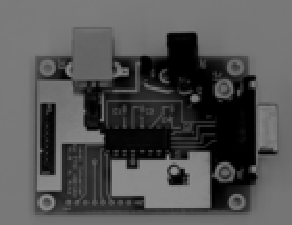
\includegraphics[width=0.3\textwidth]{./figs/pcb.pdf} &
 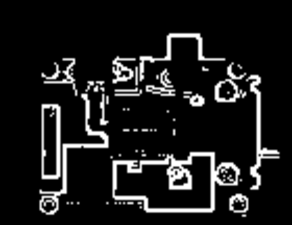
\includegraphics[width=0.3\textwidth]{./figs/pcb-res.pdf} \\
 a & b
  \end{tabular}
  \caption{Input and output images after simulation for the program given in Listing.~\ref{lst:sobel-full}}
  \label{fig:sobel-result}
\end{figure}

\section{Simulation using the SystemC backend}

SystemC simulation is performed exactly as detailed is Sec~\ref{sec:simul-using-sysc-2} (\verb|make systemc.makefile; make systemc.run|) with some
specific options, as shown in Listing~\ref{lst:sobel-proj}. The \verb|-sc_stop_when_idle| option is used to automatically
stop the simulation after a given period of inactivity (1000 ns here, \emph{i.e.} 100 clock
cycles\footnote{The default clock period is 10 ns when using the SystemC backend. This can be
  adjusted with the \texttt{sc\_clock\_period} option.}). The \verb|-sc_dump_fifo_stats| option is
used to get a precise report on FIFO occupation in order to tune the VHDL backend. The resulting
file, \verb|sobel_fifo_stats.dat| is reproduced in Listing~\ref{lst:sobel-sysc-fifos}. 
A visual inspection of the result image shows that it identical to the one obtained using the
interpreter. 

\begin{lstlisting}[style=MakeStyle,caption={Application-specific \texttt{Makefile} for simulating
    wth SystemC the application given in Listing.~\ref{lst:sobel-full}},label={lst:sobel-makef-sysc}]
SC_OPTS = -I $(CAPHLIB) -sc_abbrev_dc_ctors -sc_stop_when_idle 1000 -suppress_cast_warnings -sc_dump_fifo_stats -D ifile=pcb.txt -D threshold=80 
\end{lstlisting}
%$

\begin{lstlisting}[style=CaphStyle,caption={File \texttt{sobel\_fifo\_stats.dat} produced by the SystemC backend for 
    the application given in Listing.~\ref{lst:sobel-full}},label={lst:sobel-sysc-fifos}]
w11 fifo_size = 3
w3 fifo_size = 3
w2 fifo_size = 142
w1 fifo_size = 142
w6 fifo_size = 3
w5 fifo_size = 142
w4 fifo_size = 142
w8 fifo_size = 3
w7 fifo_size = 3
w9 fifo_size = 3
w10 fifo_size = 3
\end{lstlisting}
%$

\section{Simulation using the VHDL backend}

Again, this is very similar to what has been described in the previous chapter. The relevant line in
the project file concerns the \verb|VHDL_OPTS| macro. The \verb|-vhdl_annot_file| option is crucial
here. It gives the name of the annotation file generated by the
previous SystemC execution (\verb|sobel_fifo_stats.dat| here) to ensure correct sizing of the
FIFOs in the final VHDL design (by default, FIFOs have a depth of only 4). Concerning the
\verb|GHDL_RUN_OPTS| macro,  the value specified for
the \verb|--stop-time| option has here been derived from the final time reported by the execution of
the SystemC code (154340 ns). Simulation is a bit longer than with SystemC (about ten seconds) and
produce the same result image.

\section{VHDL synthesis}
\label{sec:vhdl-synthesis-4}

Synthesis results for the application described by the \verb|main_net.vhd| toplevel file on a Cyclone III
FPGA with Quartus II are as follows :
\begin{itemize}
\item total logic elements : 828/119088 ($<1\%$) (combinational function : 682, dedicated logic registers : 512)
\item total memory bits : 6864/3981312 ($<1\%$)
\item IO pins : 23
\item maximum clock frequency : 63.7 MHz
\end{itemize}

\section{Centered \emph{vs.} shifted convolution}
\label{sec:slight-variation}

As evidenced by Eq.~(\ref{eq:conv233}), the \verb|conv233| actor used in the previous sections
implements a so-called \emph{shifted} convolution : the output image is actually ``shifted'' one
line down and one pixel right relatively to the input image. This can be easily explained by the
fact that, since this actor operates on-the-fly on the input data streams, it can only use pixels
which are ``behind'' the current pixel. This is illustrared in Fig.~\ref{fig:shifted-conv}-a, in
which the current pixel is $y_{ij}$ and the ``past'' pixels are those shaded in gray. In this
context, the ``computation pattern'' of Eq.~(\ref{eq:conv233}) is represented by
Fig.~\ref{fig:shifted-conv}-b.  More generally, with this formulation, for a $M\times N$
convolution, the output image would be shifted $M-1$ lines down and $N-1$ pixels right.

\begin{figure}[htbp]
  \centering
  \begin{tabular}[c]{cc}
    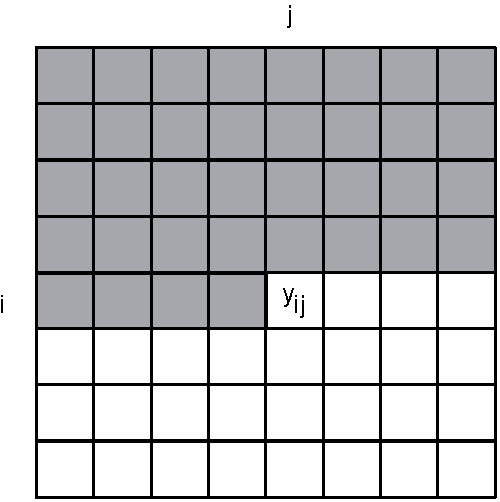
\includegraphics[width=0.3\textwidth]{./figs/conv-a.pdf} &
    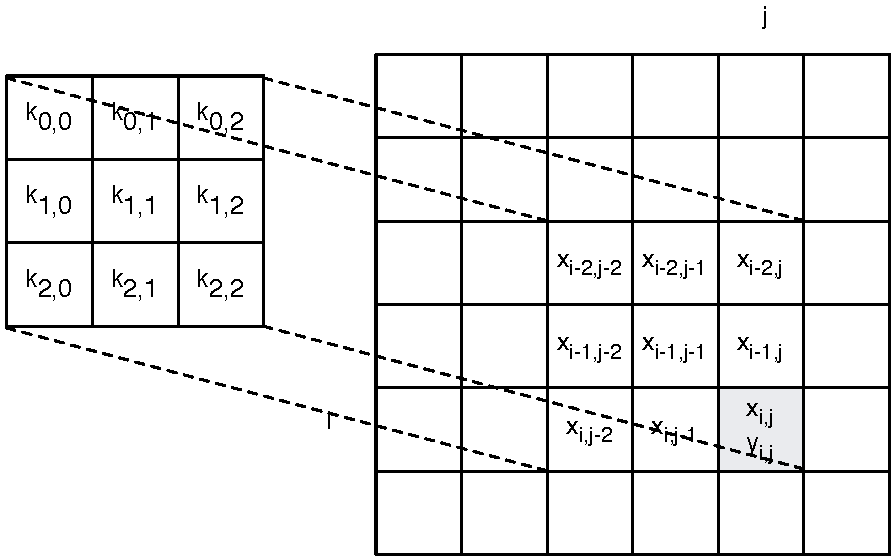
\includegraphics[width=0.5\textwidth]{./figs/conv-b.pdf} \\
-a- & -b-
  \end{tabular}
  \caption{Shifted convolution}
  \label{fig:shifted-conv}
\end{figure}

In certain situations, this ``shifting'' effect is not desirable and one would prefer a more
classical definition of the convolution, in which the convolution kernel is ``centered'' around the
current pixel, as illustrated in Fig.~\ref{fig:centered-conv}. The CAPH standard library therefore
provides ``centered'' versions of 1D and 2D convolutions for several kernel dimensions. The program
\texttt{mkconv}, described in App F of the reference manual, also has an option to generate centered
convolution for any (odd) kernel dimensions.

\begin{figure}[htbp]
\centering
    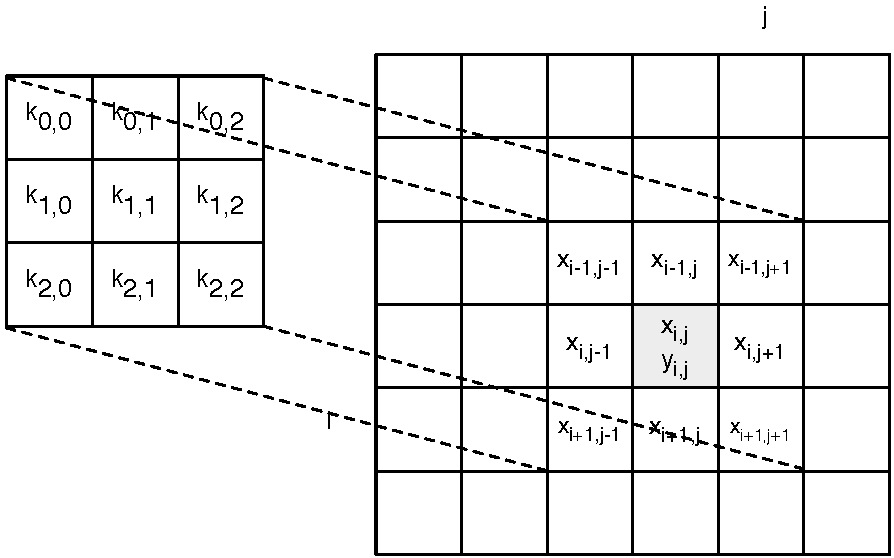
\includegraphics[width=0.5\textwidth]{./figs/cconv.pdf}
  \caption{Centered convolution}
  \label{fig:centered-conv}
\end{figure}

In our case, the only modification is to replace the \verb|conv233| actor in
Listing~\ref{lst:sobel-full} by its centered counterpart \verb|cconv233|. This modification is
denoted in Listing~\ref{lst:sobel-full2} (in which only modified lines have been reproduced).
 
\begin{lstlisting}[style=CaphStyle,numbers=left,caption={Modification of
    listing~\ref{lst:sobel-full} to use \emph{centered} convolution},label={lst:sobel-full2}]
...
net gx = cconv233 ([[1,0,-1], [2,0,-2], [1,0,-1]], 0, 0) i;
net gy = cconv233 ([[1,2,1], [0,0,0], [-1,-2,-1]], 0, 0) i;
...
\end{lstlisting}

\medskip
Simulation results with the interpreter are unchanged, except for the result image, which of course is no longer
shifted and the channel occupation report, as shown in Listing~\ref{lst:sobel-fifo-occ2}.

\begin{lstlisting}[style=BashOutputStyle,caption={FIFO occupation reported by the interpreter for
    the application using centered convolution actors},label={lst:sobel-fifo-occ2}]
W3: occ=0/256 max=107
W2: occ=0/256 max=143
W1: occ=0/256 max=143
W6: occ=0/256 max=107
W5: occ=0/256 max=143
W4: occ=0/256 max=143
W8: occ=0/256 max=2
W7: occ=0/256 max=2
W9: occ=0/256 max=2
W10: occ=0/256 max=2
\end{lstlisting}

Note that, compared with the results obtained with the shifted convolution actors, the occupation of
channels \texttt{W3} and \texttt{W6} can now grow to 107 places. A visualisation of the application
dataflow graph (with the \verb|-dot| and \verb|-dot_show_indexes| options) shows that these channels
are those connecting the \texttt{i} input to the \texttt{cconv233} actors. The reasons for this is
that \emph{centered} convolution actors, contrary to \emph{shifted} convolution actors, requires a
``flushing'' phase at the end of each line of the image and the end of each image. This phase is
needed to empty the FIFOs which are used to memorize previous lines and pixels. During this phase,
no input can be read and if any are available, they accumulates on the FIFOs connected to the actor
inputs. 

\medskip
The same behavior can be observed with the SystemC simulation : the file \verb|main_fifo_stats.dat|
obtained with option \verb|-sc_dump_fifo_stats| reports a maximum occupation of 108 for the two
FIFOs connecting input \texttt{i} to the actors \texttt{cconv233}\footnote{The difference of 1 with
  the value obtained with the interpreter is not significant here.}.  As explained in Sec.~9.5.5 of
the reference manual, this ``accumulation'' effect can be eliminated by inserting \emph{blanking}
clock cycles at the end of each line and each image. If one pixel is injected per clock period, the
amount of horizontal (resp. blanking) for a $M\times N$ convolution should be equal to $N$ (resp
$L\times (M-1)/2$), where $L$ is the width of the input images (number of pixel per column). In our
case, this gives respective values of 5 and 140. This is achieved by modifying the SystemC-related
options in the project file as
illustrated in Listing~\ref{lst:sobel-proj-2}. Note that we also had to increase the ``idle
time'' used to detect the end of the simulation because of the inserted blanking cycles.


\begin{lstlisting}[style=MakeStyle,caption={Modified project file for SystemC simulation (with
    centered convolution actors and blanking)},label={lst:sobel-proj-2}]
...
SC_OPTS = -D ifile=pcb.txt -D threshold=80 -sc_abbrev_dc_ctors -sc_stop_when_idle 2000 -suppress_cast_warnings -sc_dump_fifo_stats -sc_istream_hblank 4 -sc_istream_vblank 140
...
\end{lstlisting}
%$

\medskip
Blanking can also -- and actually should if simulation is expected to reflect ``real'' behavior on the
target hardware, as explained in Sec 9.5.5 of the reference manual -- be simulated at the VHDL
level. For this, the \verb|-vhdl_istream_blanking| must be passed to the CAPH compiler and the
option \texttt{-hblank} (resp. \texttt{vblank}) passed to \texttt{txt2bin} program. This is here
achieved by modifying the project file as illustrated in Listing~\ref{lst:sobel-proj-3}.

\begin{lstlisting}[style=MakeStyle,caption={Modified project file for VHDL simulation (with
    centered convolution actors and blanking)},label={lst:sobel-proj-3}]
...
VHDL_OPTS = -D ifile=pcb.pgm -D threshold=80 -suppress_cast_warnings -vhdl_annot_file main_fifo_stats.dat -vhdl_istream_blanking
...
\end{lstlisting}
%$

%%% Local Variables: 
%%% mode: latex
%%% TeX-master: "caph-primer"
%%% End: 



\begin{thebibliography}{1}

\bibitem{caph-lrm}
J.~S\'erot.
\newblock CAPH Reference Manual.
\newblock Available online at \url{caph.univ-bpclermont.fr}

\bibitem{Graphviz}
\newblock The \texttt{Graphviz} Graph Visualization Software.
\newblock Available online at \url{www.graphviz.org}

\bibitem{GHDL}
\newblock The GHDL VHDL Simulator.
\newblock Available online at \url{gna.org/projects/ghdl}

\bibitem{gtkwave}
\newblock The GTKWave Software.
\newblock Available online at \url{gtkwave.sourceforge.net}

\bibitem{VCD}
\newblock The Value Change Dump file format.
\newblock \url{en.wikipedia.org/wiki/Value_change_dump}

\bibitem{PGM}
\newblock The NetPBM grayscale file format.
\newblock \url{netpbm.sourceforge.net/doc/pgm.html}

\bibitem{GpStudio}
\newblock GpStudio : a Toolchain for FPGA-based smart camera.
\newblock \url{gpstudio.univ-bpclermont.fr}

\bibitem{MinGW}
\newblock Minimalist GNU for Windows
\newblock \url{www.mingw.org}

\bibitem{CygWin}
\newblock Linux for Windows
\newblock \url{www.cygwin.com}

 
\end{thebibliography}
\tableofcontents

\end{document}
